\documentclass[]{book}
\usepackage{lmodern}
\usepackage{amssymb,amsmath}
\usepackage{ifxetex,ifluatex}
\usepackage{fixltx2e} % provides \textsubscript
\ifnum 0\ifxetex 1\fi\ifluatex 1\fi=0 % if pdftex
  \usepackage[T1]{fontenc}
  \usepackage[utf8]{inputenc}
\else % if luatex or xelatex
  \ifxetex
    \usepackage{mathspec}
  \else
    \usepackage{fontspec}
  \fi
  \defaultfontfeatures{Ligatures=TeX,Scale=MatchLowercase}
\fi
% use upquote if available, for straight quotes in verbatim environments
\IfFileExists{upquote.sty}{\usepackage{upquote}}{}
% use microtype if available
\IfFileExists{microtype.sty}{%
\usepackage[]{microtype}
\UseMicrotypeSet[protrusion]{basicmath} % disable protrusion for tt fonts
}{}
\PassOptionsToPackage{hyphens}{url} % url is loaded by hyperref
\usepackage[unicode=true]{hyperref}
\hypersetup{
            pdftitle={Metody przetwarzania danych meteorologicznych w języku programowania R},
            pdfborder={0 0 0},
            breaklinks=true}
\urlstyle{same}  % don't use monospace font for urls
\usepackage{natbib}
\bibliographystyle{apalike}
\usepackage{color}
\usepackage{fancyvrb}
\newcommand{\VerbBar}{|}
\newcommand{\VERB}{\Verb[commandchars=\\\{\}]}
\DefineVerbatimEnvironment{Highlighting}{Verbatim}{commandchars=\\\{\}}
% Add ',fontsize=\small' for more characters per line
\usepackage{framed}
\definecolor{shadecolor}{RGB}{248,248,248}
\newenvironment{Shaded}{\begin{snugshade}}{\end{snugshade}}
\newcommand{\KeywordTok}[1]{\textcolor[rgb]{0.13,0.29,0.53}{\textbf{#1}}}
\newcommand{\DataTypeTok}[1]{\textcolor[rgb]{0.13,0.29,0.53}{#1}}
\newcommand{\DecValTok}[1]{\textcolor[rgb]{0.00,0.00,0.81}{#1}}
\newcommand{\BaseNTok}[1]{\textcolor[rgb]{0.00,0.00,0.81}{#1}}
\newcommand{\FloatTok}[1]{\textcolor[rgb]{0.00,0.00,0.81}{#1}}
\newcommand{\ConstantTok}[1]{\textcolor[rgb]{0.00,0.00,0.00}{#1}}
\newcommand{\CharTok}[1]{\textcolor[rgb]{0.31,0.60,0.02}{#1}}
\newcommand{\SpecialCharTok}[1]{\textcolor[rgb]{0.00,0.00,0.00}{#1}}
\newcommand{\StringTok}[1]{\textcolor[rgb]{0.31,0.60,0.02}{#1}}
\newcommand{\VerbatimStringTok}[1]{\textcolor[rgb]{0.31,0.60,0.02}{#1}}
\newcommand{\SpecialStringTok}[1]{\textcolor[rgb]{0.31,0.60,0.02}{#1}}
\newcommand{\ImportTok}[1]{#1}
\newcommand{\CommentTok}[1]{\textcolor[rgb]{0.56,0.35,0.01}{\textit{#1}}}
\newcommand{\DocumentationTok}[1]{\textcolor[rgb]{0.56,0.35,0.01}{\textbf{\textit{#1}}}}
\newcommand{\AnnotationTok}[1]{\textcolor[rgb]{0.56,0.35,0.01}{\textbf{\textit{#1}}}}
\newcommand{\CommentVarTok}[1]{\textcolor[rgb]{0.56,0.35,0.01}{\textbf{\textit{#1}}}}
\newcommand{\OtherTok}[1]{\textcolor[rgb]{0.56,0.35,0.01}{#1}}
\newcommand{\FunctionTok}[1]{\textcolor[rgb]{0.00,0.00,0.00}{#1}}
\newcommand{\VariableTok}[1]{\textcolor[rgb]{0.00,0.00,0.00}{#1}}
\newcommand{\ControlFlowTok}[1]{\textcolor[rgb]{0.13,0.29,0.53}{\textbf{#1}}}
\newcommand{\OperatorTok}[1]{\textcolor[rgb]{0.81,0.36,0.00}{\textbf{#1}}}
\newcommand{\BuiltInTok}[1]{#1}
\newcommand{\ExtensionTok}[1]{#1}
\newcommand{\PreprocessorTok}[1]{\textcolor[rgb]{0.56,0.35,0.01}{\textit{#1}}}
\newcommand{\AttributeTok}[1]{\textcolor[rgb]{0.77,0.63,0.00}{#1}}
\newcommand{\RegionMarkerTok}[1]{#1}
\newcommand{\InformationTok}[1]{\textcolor[rgb]{0.56,0.35,0.01}{\textbf{\textit{#1}}}}
\newcommand{\WarningTok}[1]{\textcolor[rgb]{0.56,0.35,0.01}{\textbf{\textit{#1}}}}
\newcommand{\AlertTok}[1]{\textcolor[rgb]{0.94,0.16,0.16}{#1}}
\newcommand{\ErrorTok}[1]{\textcolor[rgb]{0.64,0.00,0.00}{\textbf{#1}}}
\newcommand{\NormalTok}[1]{#1}
\usepackage{longtable,booktabs}
% Fix footnotes in tables (requires footnote package)
\IfFileExists{footnote.sty}{\usepackage{footnote}\makesavenoteenv{long table}}{}
\usepackage{graphicx,grffile}
\makeatletter
\def\maxwidth{\ifdim\Gin@nat@width>\linewidth\linewidth\else\Gin@nat@width\fi}
\def\maxheight{\ifdim\Gin@nat@height>\textheight\textheight\else\Gin@nat@height\fi}
\makeatother
% Scale images if necessary, so that they will not overflow the page
% margins by default, and it is still possible to overwrite the defaults
% using explicit options in \includegraphics[width, height, ...]{}
\setkeys{Gin}{width=\maxwidth,height=\maxheight,keepaspectratio}
\IfFileExists{parskip.sty}{%
\usepackage{parskip}
}{% else
\setlength{\parindent}{0pt}
\setlength{\parskip}{6pt plus 2pt minus 1pt}
}
\setlength{\emergencystretch}{3em}  % prevent overfull lines
\providecommand{\tightlist}{%
  \setlength{\itemsep}{0pt}\setlength{\parskip}{0pt}}
\setcounter{secnumdepth}{5}
% Redefines (sub)paragraphs to behave more like sections
\ifx\paragraph\undefined\else
\let\oldparagraph\paragraph
\renewcommand{\paragraph}[1]{\oldparagraph{#1}\mbox{}}
\fi
\ifx\subparagraph\undefined\else
\let\oldsubparagraph\subparagraph
\renewcommand{\subparagraph}[1]{\oldsubparagraph{#1}\mbox{}}
\fi

% set default figure placement to htbp
\makeatletter
\def\fps@figure{htbp}
\makeatother

\usepackage{polski}
\usepackage[utf8]{inputenc}
\usepackage{booktabs}
\usepackage{amsthm}
\linespread{1.3}
\makeatletter
\def\thm@space@setup{%
  \thm@preskip=8pt plus 2pt minus 4pt
  \thm@postskip=\thm@preskip
}
\makeatother
\newenvironment{foo}
    {\begin{center}
    \begin{tabular}{|p{0.9\textwidth}|}
    \hline\\
    }
    {
    \\\\\hline
    \end{tabular}
    \end{center}
    }

\title{Metody przetwarzania danych meteorologicznych w języku programowania R}
\author{Bartosz Czernecki}
\date{}

\usepackage{amsthm}
\newtheorem{theorem}{Twierdzenie}[chapter]
\newtheorem{lemma}{Lemma}[chapter]
\theoremstyle{definition}
\newtheorem{definition}{Definition}[chapter]
\newtheorem{corollary}{Corollary}[chapter]
\newtheorem{proposition}{Proposition}[chapter]
\theoremstyle{definition}
\newtheorem{example}{Example}[chapter]
\theoremstyle{definition}
\newtheorem{exercise}{Exercise}[chapter]
\theoremstyle{remark}
\newtheorem*{remark}{Remark}
\newtheorem*{solution}{Solution}
\begin{document}
\maketitle

{
\setcounter{tocdepth}{1}
\tableofcontents
}
\chapter*{Wprowadzenie}\label{wprowadzenie}
\addcontentsline{toc}{chapter}{Wprowadzenie}

Przetwarzanie danych to niezwykle szeroka dyscyplina wymagająca
praktycznego zastosowania szeregu umiejętności w celu poprawnego
zrozumienia i interpretacji analizowanych zbiorów danych.

Każdego dnia gromadzone są petabajty nowych informacji związanych z
monitoringiem atmosfery. Przetwarzanie choćby niewielkiego wycinka z
nich wymaga często stosowania złożonych algorytmów postępowania. Te z
kolei wymuszają stosowanie odpowiednich narzędzi obliczeniowych, których
poznanie jest procesem długotrwałym, wykraczającym najczęściej poza
pojedynczy podręcznik lub kurs.

Mając na uwadze powyższe przesłanki nadrzędnym celem niniejszego skryptu
jest przede wszystkim zaznajomienie z ``narzędziami'' języka
programowania R do analizy i wizualizacji danych, które pozwolą Tobie na
dalsze samodoskonalenie nabytych umiejętności.

``Analiza danych, a w szczególności analiza z użyciem programu
\textbf{R}, charakteryzuje się stromą krzywą uczenia. Na początku wiele
rzeczy będzie nowych i trudnych. Gwarantuję jednak, że wysiłek włożony w
poznawanie programu R opłaci się. Z czasem będziesz coraz sprawniej
przetwarzać i wizualizować dane, a elastyczność i ekspresja programu R
powodują, że praktycznie nie będzie przed Tobą barier związanych z
analizą najróżniejszych danych'' \citep{biecek2016} \ldots{} nie tylko
meteorologicznych\ldots{}

\chapter{\texorpdfstring{\textbf{R}}{R}}\label{whyr}

\section{\texorpdfstring{Kilka słów o \textbf{R}
\ldots{}}{Kilka słów o R \ldots{}}}\label{kilka-sow-o-r}

\textbf{R} to bardzo dynamicznie rozwijający się język programowania
używany przede wszystkim do analiz statystycznych, przetwarzania i
wizualizacji danych. Jego rosnąca w ostatnich latach popularność jest
związana przynajmniej z kilkoma czynnikami. Oto niektóre z nich:

\begin{itemize}
\item
  W porównaniu do wielu innych języków programowania nauka \textbf{R}
  jest często dużo łatwiejsza (głównie dzięki relatywnie łatwej składni
  i interaktywności związanej z brakiem konieczności kompilacji).
\item
  Popularność \textbf{R} mocno poszybowała w górę od czasu wydania
  zintegrowanego środowiska programistycznego (IDE) \textbf{RStudio},
  które w znacznym stopniu usprawnia komfort pracy.
\item
  Multiplatformość - \textbf{R} można uruchamić na niemal każdym
  współczesnym systemie operacyjnym (Windows, Mac OS, Linux/UNIX),
  zarówno na komputerach PC, jak i na dużych klastrach obliczeniowych.
\item
  \textbf{R} jest oprogramowaniem bezpłatnym i otwartoźródłowym -
  oznacza to, że korzystanie z \textbf{R} oraz modyfikowanie kodu na
  mocy licencji GPL nie nastręcza dodatkowych kosztów. Małe firmy tną w
  ten sposób koszty, giganci (m.in. Google, Yahoo, Facebook, Microsoft,
  NYSE, Wirtualna Polska, itp.) dostosowują rozwiązania bazujące na
  \textbf{R} do własnych potrzeb.
\item
  \textbf{R} jest językiem programowania, co oznacza że nawet jeśli nie
  ma interesującego nas algorytmu w natywnie zainstalowanym \textbf{R}
  możemy takie narzędzie stworzyć samemu. Najczęściej jednak okazuje
  się, że ktoś inny napisał już analogiczne lub podobne rozwiązanie i
  opublikował je w postaci pakietu programistycznego, który możemy
  bezpłatnie wykorzystać. Obecnie w serwisie CRAN znajduje się ponad
  10000(!) takich pakietów dedykowanych dla szerokiego grona odbiorców.
\item
  Liczba danych na których możemy jednocześnie pracować w standardowych
  rozwiązaniach ograniczona jest jedynie pamięcią RAM (dla wersji
  64-bitowej). Obecnie jest to ok. 1-2 rzędy wielkości więcej w
  porównaniu do najczęściej stosowanych arkuszy kalkulacyjnych
  \citep{excel2016}.
\item
  W przypadku napotkania problemów możemy skorzystać z pomocy
  społeczności użytkowników \textbf{R}, którzy bardzo szybko reagują na
  forach dyskusyjnych (np.
  \href{http://stackoverflow.com/}{stackoverflow}.
\item
  \ldots{}
\end{itemize}

To tylko część z zalet związanych z stosowaniem środowiska
programistycznego \textbf{R} do przetwarzania danych. Z punktu widzenia
analizy danych meteorologicznych niezwykle istotne staje się
wykorzystanie jednego środowiska pracy zamiast kilku oddzielnych
aplikacji. W \textbf{R} możliwe jest jednoczesne zautomatyzowanie
procesu pobierania i wstępnego przygotowania (czyszczenia) danych,
rozbudowanej analizy statystycznej danych (także wielowymiarowych),
wykorzystania różnych formatów danych (w tym np. GIS) i wykonania analiz
czasowo-przestrzennych z finalną konwersją i wizualizacją danych w
postaci statycznych lub interaktywnych rozwiązań.

W odróżnieniu od zwykle wykorzystywanych arkuszy kalkulacyjnych praca w
\textbf{R} pozwala na dużą dozę automatyzacji całego procesu eksploracji
danych od momentu ich importu do środowiska \textbf{R}, poprzez ich
weryfikację i czyszczenie, transformację do wybranego formatu i
skończywszy na etapie wizualizacji (ewentualnego
modelowania/prognozowania) oraz końcowego przekazu do odbiorców
końcowych \citep{wickham2016}.

\begin{figure}
\centering
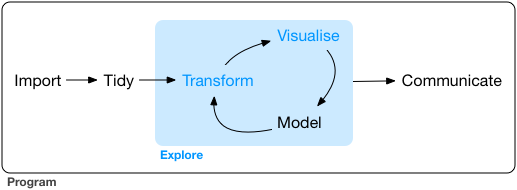
\includegraphics{figures/data-science-explore.png}
\caption{Typowy przebieg kolejnych etapów \emph{data science} według
Hadleya Wickhama \citep{wickham2016}}
\end{figure}

\section{\texorpdfstring{Dlaczego warto uczyć się
\textbf{R}?}{Dlaczego warto uczyć się R?}}\label{dlaczego-warto-uczyc-sie-r}

Prawdopodobnie dotychczas do Twojej pracy z danymi wystarczała znajomość
obsługi arkusza kalkulacyjnego, gdzie wszystkie dane swobodnie mieściły
się w pojedynczym arkuszu i mogłeś je jednocześnie poukładać według
własnego uznania i wizualizować za pomocą intuicyjnego, klikanego
interfejsu graficznego. Filozofia pracy w \textbf{R} zdecydowanie różni
się od powyższego schematu postępowania. \textbf{R} jest językiem
programowania, co dla osób nie posiadających wcześniejszego
przygotowania programistycznego oznacza mozolne poznawanie specyficznej
składni i funkcji programistycznych.

Oznacza to także konieczność porzucenia własnych przyzwyczajeń. Jest to
trudne, zwłaszcza na początku i wymaga wielu godzin wytężonej pracy
połączonej z twórczym eksperymentowaniem i korygowaniem niezliczonej
liczby własnych błędów. Z pewnością jednak spędzony czas przy nauce
\textbf{R} jest w relatywnie krótkim okresie rekompensowany z nawiązką,
a analiza danych uprzednio zajmująca długie godziny często skraca się do
czasu wykonywania pojedynczej linii kodu.

Umiejętność programowania w \textbf{R} jest coraz częściej doceniana na
rynku pracy, co pokazuje rosnąca liczba ofert dla kandydatów z
zaawansowaną obsługą środowiska \textbf{R}. Ten trend obserwuje się
także w środowiskach naukowych oraz we wiodących ośrodkach badań
atmosfery, gdzie \textbf{R} i blisko pokrewne języki wysokiego poziomu
stają się \emph{lingua franca} analizy danych.

\section{\texorpdfstring{X przykazań nauki
\textbf{R}}{X przykazań nauki R}}\label{x-przykazan-nauki-r}

Choć nie ma uniwersalnej recepty na naukę \textbf{R} warto pamiętać o
poniższych wskazówkach, które pomogą w początkowych etapach pracy:

\begin{foo}
\begin{enumerate}
\def\labelenumi{\arabic{enumi}.}
\tightlist
\item
  Nie bój się stromej krzywej uczenia (rys. \ref{fig:krzywauczenia}).
  Efektywna nauka programowania wymaga długich godzin praktyki.
  Eksperymentuj z różnymi kombinacjami składni, które przyjdą Ci do
  głowy i sprawdzaj ich wyniki.
\item
  Interpretuj błędy pojawiające się po każdej błędnej komendzie.
\item
  Pracuj na własnych, dobrze znanych zbiorach danych. Łatwiej będzie Ci
  zrozumieć działanie poszczególnych funkcji i wyłapać ewentualne błędy.
\item
  Staraj się unikać początkowo dużych zbiorów danych jeśli nie jest to
  wymagane.
\item
  Korzystaj z systemu pomocy zarówno wbudowanej natywnie, jak i
  dostępnej online (google oraz stackoverflow).
\item
  Zrozumienie podstaw jest kluczowe aby analizować bardziej
  skomplikowane przypadki (dające dużo większą satysfakcję).
\item
  Twórz możliwie dużo i możliwie jak najbardziej opisowych komentarzy.
\item
  Staraj się utrzymywać odpowiedni porządek w składni tworzonego kodu
  oraz w nazwach plików.
\item
  R nie jest środowiskiem idealnym do wszystkich zastosowań. Prowadzenie
  budżetu domowego czy stworzenie pojedynczej, poprawnej kartograficznie
  mapy jest prawdopodobnie łatwiejsze i szybsze w innych programach.
\item
  Rób przerwy. Czasem najlepsze pomysły przychodzą w najmniej
  oczekiwanych momentach. Niekoniecznie przy komputerze.
\end{enumerate}
\end{foo}

\label{fig:krzywauczenia}

\begin{verbatim}
## Warning in title(...): conversion failure on 'Poziom umiejętności' in
## 'mbcsToSbcs': dot substituted for <c4>
\end{verbatim}

\begin{verbatim}
## Warning in title(...): conversion failure on 'Poziom umiejętności' in
## 'mbcsToSbcs': dot substituted for <99>
\end{verbatim}

\begin{verbatim}
## Warning in title(...): conversion failure on 'Poziom umiejętności' in
## 'mbcsToSbcs': dot substituted for <c5>
\end{verbatim}

\begin{verbatim}
## Warning in title(...): conversion failure on 'Poziom umiejętności' in
## 'mbcsToSbcs': dot substituted for <9b>
\end{verbatim}

\begin{figure}

{\centering 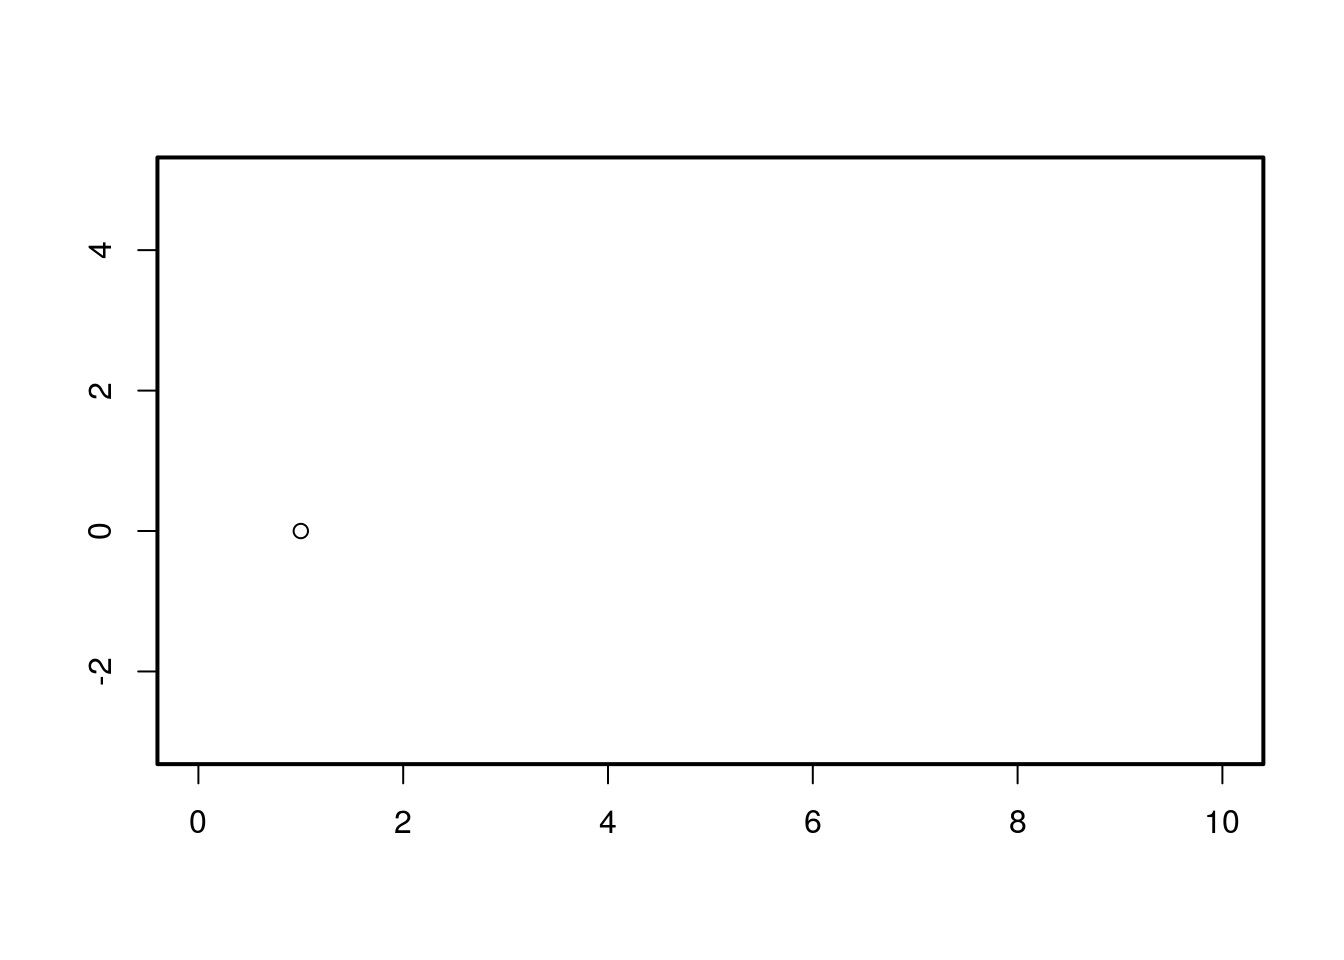
\includegraphics[width=0.8\linewidth]{ksiazka_files/figure-latex/unnamed-chunk-2-1} 

}

\caption{Porównanie stromej krzywej uczenia **R** i arkuszy kalkulacyjnych}\label{fig:unnamed-chunk-2}
\end{figure}

~

~

\section{Od czego zacząć?}\label{od-czego-zaczac}

Tematyce programowania w \textbf{R} poświęcono sporą liczbę
podręczników, artykułów naukowych oraz \emph{internetowych tutoriali}
omawiających tajniki \emph{data science}. Stanowią one cenne uzupełnie
niniejszego kursu, który wiele zagadnień (zwłaszcza technicznych)
traktuje bardzo pobieżnie.

Spośród dostępnych źródeł książkowych opublikowanych w języku polskim na
szczególną uwagę zasługują przede wszystkim podręczniki:

\begin{itemize}
\tightlist
\item
  Przewodnik po pakiecie R \citep{biecek2008} - najbardziej popularny
  podręcznik w Polsce, dostępny w kilku różnych wydaniach z których
  najłatwiejsze powinno być ostatnie (2017). Pierwsze rozdziały dostępne
  bezpłatnie na stronie autora \href{www.biecek.pl/R}{biecek.pl/R}.
\item
  Programowanie w języku R. Analiza danych, obliczenia, symulacje
  \citep{gagolewski2016} - podręcznik zdecydowanie bardziej zaawansowany
  technicznie, rekomendowany dla osób mających wcześniejszy kontakt z
  programowaniem. Dostępny bezpłatnie ze strony internetowej biblioteki
  uniwersyteckiej UAM.
\item
  Geostatystyka w R \citep{nowosad2016} - Książka opisująca rozszerzone
  standardy modelowania GIS. Dostępna bezpłatnie na stronie
  \url{https://bookdown.org/nowosad/Geostatystyka/}.
\item
  Skrypt wprowadzający do R udostępniony na stronie internetowej Zakładu
  Klimatologii UAM - jest to bardzo krótkie wprowadzenie do \textbf{R} w
  dużym w zarysie prezentujące najważniejsze elementy niezbędne do pracy
  w tym środowisku. \url{http://klimat.amu.edu.pl/?page_id=2500}.
\end{itemize}

oraz

\begin{itemize}
\tightlist
\item
  An Introduction to R \citep{rintro2004} - aktualizowany na biężaco
  oficjalny podręcznik deweloperów \citep{r2016} omawiający podstawowe
  aspekty pracy w \textbf{R}.
\end{itemize}

Kursy:

\begin{itemize}
\tightlist
\item
  Pogromcy danych: \url{pogromcydanych.icm.edu.pl} - dwuczęsciowy kurs
  internetowy autorstwa Przemysława Biecka będący wprowadzeniem do
  zagadnień \emph{data science} w \textbf{R}
\item
  Coursera: dostępnych przynajmniej kilka kursów internetowych
  związanych z przetwarzaniem danych z \textbf{R} \url{coursera.org}.
\end{itemize}

\chapter{\texorpdfstring{Podstawy
\textbf{R}}{Podstawy R}}\label{podstawy-r}

Praca w środowisku R możliwa jest w dwóch podstawowych trybach:
skryptowym (wsadowym) oraz interaktywnym. Tryb interaktywny jest mniej
skomplikowany i od niego rozpoczniemy naszą naukę. Praca w tym trybie
polega na wprowadzaniu komend do konsoli (interpretera języka
programowania), który znajduje się domyślnie po lewej stronie okna
programu \textbf{RStudio}.

\begin{figure}
\centering
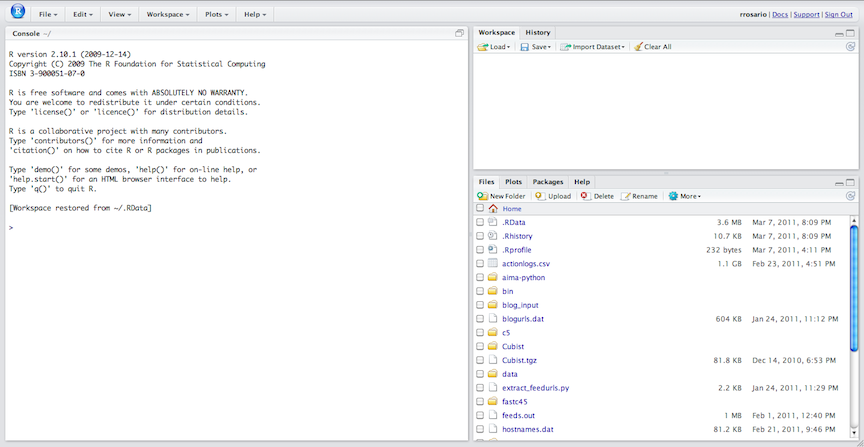
\includegraphics{figures/rstudio.png}
\caption{Ekran początkowy programu \textbf{RStudio}}
\end{figure}

\section{Terminal R}\label{terminal-r}

W konsoli R możemy wpisywać komendy, a po naciśnięciu klawisza
\emph{Enter} komendy te są przez komputer interpretowane. Jeśli
polecenie jest poprawne komputer obliczy jego rezultat. Alternatywnie
informacja zwrotna o napotkanym błędzie wyświetlana jest jako
\emph{error} lub w formie ostrzeżenia (ang. \emph{warning})). Spróbujmy
wykorzystać R jako kalkulator i przetestujmy zachowanie terminala.

\begin{Shaded}
\begin{Highlighting}[]
\DecValTok{5}\OperatorTok{+}\DecValTok{3}
\end{Highlighting}
\end{Shaded}

\begin{verbatim}
## [1] 8
\end{verbatim}

Brak informacji o błędzie oznacza poprawne wykonanie działania. Obok
wyniku w nawiasie kwadratowym komputer zwrócił liczbę porządkową
pierwszej wartości w danym wierszu.

\begin{Shaded}
\begin{Highlighting}[]
\DecValTok{5}\OperatorTok{+}\DecValTok{2}\NormalTok{,}\DecValTok{5}
\end{Highlighting}
\end{Shaded}

\begin{verbatim}
## Error: <text>:1:4: unexpected ','
## 1: 5+2,
##        ^
\end{verbatim}

Komunikat błędu wskazuje miejsce jego wystąpienia. W tym przypadku jest
to przecinek, który nie pasuje do składni interpretowanego polecenia,
ponieważ separatorem miejsc dziesiętnych w R jest kropka a nie
przecinek.

\begin{quote}
Jeśli chcemy szybko poprawić ten błąd możemy użyć kursorów (strzałek) na
klawiaturze góra-dół do przeglądania ostatnio wprowadzonych poleceń i
kursorami lewo-prawo przenieść się do miejsca wymagającego poprawy.
\end{quote}

Zwróć uwagę, że jeśli komenda jest (przynajmniej częściowo) poprawna,
ale nie zostanie zakończona w danej linii, wówczas po naciśnięciu
\emph{Entera} zamiast tzw. znaku zachęty \texttt{"\textgreater{}"}
zostanie zwrócony znak \texttt{"+"}.

\begin{figure}
\centering
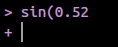
\includegraphics{figures/niedokonczona_komenda.png}
\caption{Przykład niepoprawnie zakończonej komendy (brak znaku ``)'' ),
i pojawienie się znaku ``+'' w nowej linii konsoli oznaczający możliwość
dokończenia wpisywanej komendy}
\end{figure}

W takiej sytuacji możliwe są 2 rozwiązania - dokończenie wpisywania
poprzedniej komendy, lub naciśnięcie klawisza \emph{Esc} w celu
przerwania bieżącego procesu. Klawisz \emph{Esc} (lub ikonkę
symbolizującą znak \emph{STOP}) można nacisnąć zawsze w celu przerwania
aktualnie aktywnego procesu.

\textbf{Zadanie:}

Sprawdź powyższe działania terminala testując polecenie: \texttt{6+}
(\emph{Enter}), w kolejnej linii wprowadź dowolną liczbę i ponownie
naciśnij \emph{Enter}. Za drugim razem wpisz \texttt{6+} (\emph{Enter}),
ale tym razem przerwij działanie stosując \emph{Esc}.

~

~

\section{Arytmetyka}\label{arytmetyka}

Wykonaj poniższe zadania sprawdzające działanie \textbf{R} jako
kalkulatora:

\begin{enumerate}
\def\labelenumi{\arabic{enumi}.}
\tightlist
\item
  Oblicz wyrażenie \texttt{2+3*5}
\item
  Stosując nawiasy, które pozwalają na zmianę domyślnej kolejności
  wykonywania działań zmodyfikuj powyższe działanie w taki sposób, aby
  najpierw była wykonywane sumowanie, a dopiero potem mnożenie (tj.,
  końcowy wynik powinien dać 25)
\item
  Pomnóż liczby 3 i 5
\item
  Podziel dowolne 2 liczby
\item
  Sprawdź działanie operatorów \texttt{\%\%} oraz \texttt{\%/\%} na
  dowolnych dwóch liczbach całkowitych. Do czego one służą?
\item
  Sprawdź działanie operatora \texttt{\^{}}
\end{enumerate}

Jeśli chcesz obliczyć wynik funkcji wykładniczej (\texttt{exp}), sinusa
(\texttt{sin}), cosinusa (\texttt{cos}), pierwiastka kwadratowego
(\texttt{sqrt}), logarytmu dziesiętnego (\texttt{log}), wartości
bezwzględnej (\texttt{abs}), wartości maksymalnej (\texttt{max}),
minimalnej (\texttt{min}), średniej (\texttt{mean}), odchylenia
standardowego (\texttt{sd}), itp., musisz zastosować składnię funkcyjną,
o której powiemy nieco później. W najprostszej postaci należy wprowadzić
nazwę funkcji i w nawiasie podać argument dla funkcji, czyli w tym
przypadku liczbę.

\textbf{UWAGA!} Wielkość znaków w \textbf{R} MA ZNACZENIE! (czyli
\texttt{LOG} to dla komputera coś innego niż \texttt{log}).

\begin{quote}
W RStudio bardzo przydatny jest klawisz tabulatora, który pozwala na
uzupełnienie nazwy funkcji lub obiektu po naciśnięciu klawisza
\emph{TAB}. W ten sposób np. po wpisaniu liter \texttt{sq} i naciśnięciu
\emph{TAB} pojawi się intuicyjne okno z podpowiedzią.
\end{quote}

\begin{enumerate}
\def\labelenumi{\arabic{enumi}.}
\setcounter{enumi}{6}
\tightlist
\item
  Na podstawie powyższych informacji oblicz:
\end{enumerate}

\begin{itemize}
\tightlist
\item
  Pierwiastek z 9
\item
  Cosinus liczby pi, gdzie \texttt{pi} jest stałą wbudowaną w R
  (wystarczy wpisać \texttt{pi} zamiast 3.141593)
\end{itemize}

\begin{enumerate}
\def\labelenumi{\arabic{enumi}.}
\setcounter{enumi}{7}
\tightlist
\item
  W jednej linii kodu podnieś liczbę 9 do kwadratu i oblicz pierwiastek
  kwadratowy (\texttt{sqrt}) z tej liczby. Podpowiedź: funkcje mogą być
  wzajemnie zagnieżdżone
\end{enumerate}

\begin{quote}
Wskazówka: Przy interpretacji polecenia R pomija spacje pomiędzy
poszczególnymi elementami działania. NIE JEST istotne czy twoja komenda
jest zapisana jako \texttt{5+4.5} czy \texttt{5\ \ \ \ +\ \ \ 4.5} (ale
nie możesz wpisać spacji przy liczbach, np.: \texttt{5+4\ \ .5} !).
\end{quote}

\section{Tworzenie obiektów}\label{tworzenie-obiektow}

Dotychczas wynik naszego polecenia wyświetlał się na ekranie, ale nie
mogliśmy z nim dalej nic zrobić, bo nie był zapisywany w pamięci
komputera. Wpisywanie komend w terminalu i sprawdzanie ich wyniku nie
jest zbyt efektywne, dlatego też większość pracy w \textbf{R} odbywa się
na obiektach. Czym jest obiekt? W bardzo dużym skrócie to po prostu
nazwa do której przypisuje się wartość. Nazwa nie może się zaczynać od
liczb oraz znaków specjalnych. Najlepiej także unikać polskich znaków.

W \textbf{R} istnieje kilka sposobów tworzenia obiektów (zmiennych).
Najczęściej stosowanym operatorem przypisania jest wyrażenie
\texttt{\textless{}-}, które w \textbf{RStudio} możemy otrzymać za
pomocą skrótu \texttt{lewy\ Alt\ +\ -}. Warto dobrze zapamiętać ten
skrót.

\begin{quote}
Obiekt można stworzyć także za pomocą operatora \texttt{=}, który działa
analogicznie jak \texttt{\textless{}-}. Ze względu na pewne
uwarunkowania historyczno-techniczne bardziej rekomendowany jest zapis w
postaci strzałki. Wyrażenie można przypisać także prawostronnie za
pomocą operatora \texttt{-\textgreater{}} . Choć jest to poprawna forma
zapisu, w praktyce jest rzadko stosowana.
\end{quote}

Stwórzmy zatem naszą pierwszą zmienną, którą nazwiemy
\texttt{temperatura} i przypiszmy jej wartość 279.15:

\begin{Shaded}
\begin{Highlighting}[]
\NormalTok{temperatura <-}\StringTok{ }\FloatTok{279.15}
\end{Highlighting}
\end{Shaded}

Zauważ, że w prawym górnym rogu okna \textbf{RStudio} w zakładce
\textbf{Environment} pojawiła nazwa zdefiniowanej zmiennej i jej
wartość. W tej zakładce będą pojawiać się wszystkie nazwy stworzonych
lub wczytanych obiektów.

W odróżnieniu od wcześniejszych zastosowań \textbf{R} jako kalkulatora
nie wyświetlił nam się wynik tej operacji. To dlatego, że zapisaliśmy go
w pamięci komputera. Brak informacji zwrotnej jednocześniej oznacza, że
operacja przebiegła poprawnie.

Jeśli chcemy wyświetlić zawartość naszej zmiennej możemy wpisać po
prostu jej nazwę lub wykorzystać funkcję \texttt{print} (pamiętaj o
używaniu \emph{TABulatora}!):

\begin{Shaded}
\begin{Highlighting}[]
\NormalTok{temperatura}
\end{Highlighting}
\end{Shaded}

\begin{verbatim}
## [1] 279.15
\end{verbatim}

\begin{Shaded}
\begin{Highlighting}[]
\KeywordTok{print}\NormalTok{(temperatura)}
\end{Highlighting}
\end{Shaded}

\begin{verbatim}
## [1] 279.15
\end{verbatim}

\begin{quote}
Pamiętaj, że wielkość znaków w \textbf{R} MA ZNACZENIE, tzn. wyrażenie
\texttt{temperatura} i \texttt{Temperatura} to dla komputera 2 różne
obiekty!
\end{quote}

Wyobraźmy sobie, że wartość przechowywana w obiekcie temperatura to
temperatura powietrza wyrażona w Kelwinach (podstawowa jednostka układu
SI). Jeśli chcemy przeliczyć Kelwiny na stopnie Celsjusza musimy
zastosować poniższe równanie \eqref{eq:konwersja}:

\begin{equation} 
  T(^\circ C) = K-273.15
  \label{eq:konwersja}
\end{equation}

W tym momencie można wykorzystać zawartość zmiennej \texttt{temperatura}
aby podstawić ją do równania i zapisać wynik działania do obiektu, który
nazwiemy \texttt{tc} (temperatura w Celsjuszach):

\begin{Shaded}
\begin{Highlighting}[]
\NormalTok{tc <-}\StringTok{ }\NormalTok{temperatura}\FloatTok{-273.15}
\end{Highlighting}
\end{Shaded}

\textbf{Zadanie:}

\begin{enumerate}
\def\labelenumi{\arabic{enumi}.}
\tightlist
\item
  Stosując poniższy wzór na przeliczenie temperatury ze stopni Celsjusza
  na temperaturę w Fahrenheitach utwórz obiekt \texttt{tf}. Wartość
  temperatury przelicz ze zmiennej \texttt{tc}
\end{enumerate}

\begin{equation} 
  T(^\circ F) = T(^\circ C) * 1.8 + 32
  \label{eq:konwersja2}
\end{equation}

\begin{enumerate}
\def\labelenumi{\arabic{enumi}.}
\setcounter{enumi}{1}
\item
  Na nowym obiekcie \texttt{tf} sprawdź działania funkcji matematycznych
  \texttt{floor}, \texttt{ceiling} oraz \texttt{round}.
\item
  Sprawdź co stanie się po wywołaniu komendy \texttt{?round} oraz
  \texttt{??"ceiling"} ?
\end{enumerate}

~

~

\section{Generowanie ciągów
liczbowych}\label{generowanie-ciagow-liczbowych}

Praca na obiektach przechowujących jedną wartość nie daje zbyt wielkich
korzyści. Obiekty R mogą przechowywać znacznie więcej wartości i aby się
o tym przekonać poznamy 3 podstawowe schematy generowania ciągów
liczbowych:

\begin{enumerate}
\def\labelenumi{\arabic{enumi}.}
\tightlist
\item
  Za pomocą \texttt{:} możemy stworzyć ciąg liczb z interwałem co 1. W
  zależności od tego jakie wartości podstawimy z prawej i lewej strony
  dwukropka będzie to ciąg rosnący lub malejący:
\end{enumerate}

\begin{Shaded}
\begin{Highlighting}[]
\DecValTok{150}\OperatorTok{:}\DecValTok{180}
\end{Highlighting}
\end{Shaded}

\begin{verbatim}
##  [1] 150 151 152 153 154 155 156 157 158 159 160 161 162 163 164 165 166
## [18] 167 168 169 170 171 172 173 174 175 176 177 178 179 180
\end{verbatim}

\begin{Shaded}
\begin{Highlighting}[]
\DecValTok{5}\OperatorTok{:-}\DecValTok{20}
\end{Highlighting}
\end{Shaded}

\begin{verbatim}
##  [1]   5   4   3   2   1   0  -1  -2  -3  -4  -5  -6  -7  -8  -9 -10 -11
## [18] -12 -13 -14 -15 -16 -17 -18 -19 -20
\end{verbatim}

\begin{Shaded}
\begin{Highlighting}[]
\FloatTok{11.375}\OperatorTok{:}\DecValTok{34}
\end{Highlighting}
\end{Shaded}

\begin{verbatim}
##  [1] 11.375 12.375 13.375 14.375 15.375 16.375 17.375 18.375 19.375 20.375
## [11] 21.375 22.375 23.375 24.375 25.375 26.375 27.375 28.375 29.375 30.375
## [21] 31.375 32.375 33.375
\end{verbatim}

\begin{enumerate}
\def\labelenumi{\arabic{enumi}.}
\setcounter{enumi}{1}
\tightlist
\item
  Podobnie do powyższego schematu działa funkcja \texttt{seq}. Szczegóły
  jej działania można znaleźć po wywołaniu komendy \texttt{?seq} (dostęp
  do systemu pomocy). Zgodnie z uzyskanymi informacjami z systemu pomocy
  - jeśli chcemy wygenerować ciąg liczb od 0 do 20 co 1 komenda będzie
  wyglądała następująco
\end{enumerate}

\begin{Shaded}
\begin{Highlighting}[]
\KeywordTok{seq}\NormalTok{(}\DataTypeTok{from=}\DecValTok{0}\NormalTok{, }\DataTypeTok{to=}\DecValTok{20}\NormalTok{, }\DataTypeTok{by=}\DecValTok{1}\NormalTok{)}
\end{Highlighting}
\end{Shaded}

\begin{verbatim}
##  [1]  0  1  2  3  4  5  6  7  8  9 10 11 12 13 14 15 16 17 18 19 20
\end{verbatim}

Jeśli nie wiemy jaki powinien być interwał pomiędzy liczbami, ale znamy
długość generowanego ciągu opcję \texttt{by} możemy zastąpić opcją
\texttt{length.out}. Jeśli chcemy wygenerować 35 liczb w równych
odległościach od 0 do 20, wówczas możemy zastosować poniższy kod:

\begin{Shaded}
\begin{Highlighting}[]
\KeywordTok{seq}\NormalTok{(}\DataTypeTok{from=}\DecValTok{0}\NormalTok{, }\DataTypeTok{to=}\DecValTok{20}\NormalTok{, }\DataTypeTok{length.out =}\DecValTok{35}\NormalTok{)}
\end{Highlighting}
\end{Shaded}

\begin{verbatim}
##  [1]  0.0000000  0.5882353  1.1764706  1.7647059  2.3529412  2.9411765
##  [7]  3.5294118  4.1176471  4.7058824  5.2941176  5.8823529  6.4705882
## [13]  7.0588235  7.6470588  8.2352941  8.8235294  9.4117647 10.0000000
## [19] 10.5882353 11.1764706 11.7647059 12.3529412 12.9411765 13.5294118
## [25] 14.1176471 14.7058824 15.2941176 15.8823529 16.4705882 17.0588235
## [31] 17.6470588 18.2352941 18.8235294 19.4117647 20.0000000
\end{verbatim}

\begin{enumerate}
\def\labelenumi{\arabic{enumi}.}
\setcounter{enumi}{2}
\tightlist
\item
  Losowe ciągi liczbowe można także wygenerować za pomocą funkcji z
  wybranych rozkładów statystycznych. Jednym z najbardziej przydatnych
  jest rozkład jednostajny ciągły, który w \textbf{R} jest wbudowany do
  funkcji \texttt{runif} lub rozkład normalny (\texttt{rnorm}).
  Przykładowo, jeśli chcemy wygenerować 5 losowych liczb w przedziale od
  1 do 10, wówczas kod wygląda następująco:
\end{enumerate}

\begin{Shaded}
\begin{Highlighting}[]
\KeywordTok{runif}\NormalTok{(}\DecValTok{5}\NormalTok{, }\DataTypeTok{min=}\DecValTok{1}\NormalTok{, }\DataTypeTok{max=}\DecValTok{10}\NormalTok{)}
\end{Highlighting}
\end{Shaded}

\begin{verbatim}
## [1] 3.147456 1.836970 6.671314 6.033624 2.028277
\end{verbatim}

\textbf{Zadanie:}

\begin{enumerate}
\def\labelenumi{\arabic{enumi}.}
\item
  W arkuszach kalkulacyjnych można wygenerować narastający ciąg liczbowy
  chwytając za róg komórki z wartością i przesuwając ją w dół. Gdybyś
  chciał wygenerować liczby od 1 do samego dołu arkusza kalkulacyjnego
  zajęło by to prawdopodobnie dużo czasu. Stwórz analogiczny schemat
  postępowania w \textbf{R} aby wygenerować ciąg liczb od 1 do 1048576 i
  zapisz ten wynik do obiektu \texttt{a}. Które z rozwiązań jest
  szybsze?
\item
  \emph{Dla chętnych:} Sprawdź ile danych w ciągu narastającym od 1
  możesz wygenerować i zapisać do obiektu \texttt{a} zanim braknie
  komputerowi pamięci? Do testów wykorzystaj wielokrotność potęgi 2 (np.
  \texttt{2\^{}20}, \texttt{2\^{}35}). Ile było by potrzebnych arkuszy
  kalkulacyjnych do przechowania takiej liczby danych gdyby każda liczba
  była zapisana w nowym rzędzie?
\item
  Stworzony obiekt niemal w całości wypełnia dostępną pamięć RAM naszego
  komputera. Usuń stworzony obiekt za pomocą funkcji \texttt{rm(a)}
\item
  Korzystając ze wzoru przeliczającego temperaturę ze stopni Celsjusza
  na stopnie Fahrenheita \eqref{eq:konwersja2} wygeneruj wartości
  temperatury w stopniach Celsjusza od -10 do +30 i oblicz ich wartości
  w stopniach Fahrenheita
\item
  Wygeneruj losowo 50 liczb o wartościach od 0 do 1 z rozkładu
  jednostajnego i oblicz wartość średnią. Funkcja do obliczania średniej
  arytmetycznej nazywa się \texttt{mean}.
\end{enumerate}

~

~

\section{Łączenie obiektów}\label{aczenie-obiektow}

Tworzenie obiektów jest możliwe także za pomocą operatora \texttt{c()},
który w \textbf{R} pozwala na sklejanie dwóch lub więcej wyrażeń (np.
liczbowych) w jedno. Fachowo taka operacja złączająca nazywa się
\emph{konkatenacją}.

Funkcja \texttt{c()} jest bardzo prosta w swoim działaniu i wymaga
podania kolejnych złączanych obiektów rozdzielonych przecinkami.
Najlepiej zaznajomić się z \emph{konkatenacją} na przykładach:

\begin{enumerate}
\def\labelenumi{\arabic{enumi}.}
\tightlist
\item
  Utwórz obiekt \texttt{a}, który będzie przechowywał wartości liczbowe
  1,2,3,5
\end{enumerate}

\begin{Shaded}
\begin{Highlighting}[]
\NormalTok{a <-}\StringTok{ }\KeywordTok{c}\NormalTok{(}\DecValTok{1}\NormalTok{,}\DecValTok{2}\NormalTok{,}\DecValTok{3}\NormalTok{,}\DecValTok{5}\NormalTok{)}
\end{Highlighting}
\end{Shaded}

\begin{enumerate}
\def\labelenumi{\arabic{enumi}.}
\setcounter{enumi}{1}
\tightlist
\item
  Utwórz obiekt \texttt{b}, który będzie zawierać wartości od 0 do 10 co
  1 oraz od 10 do 1 co 1. Wykorzystaj do tego celu operator \texttt{:}
\end{enumerate}

\begin{Shaded}
\begin{Highlighting}[]
\NormalTok{b <-}\StringTok{ }\KeywordTok{c}\NormalTok{(}\DecValTok{0}\OperatorTok{:}\DecValTok{10}\NormalTok{,}\DecValTok{10}\OperatorTok{:}\DecValTok{1}\NormalTok{)}
\end{Highlighting}
\end{Shaded}

\begin{enumerate}
\def\labelenumi{\arabic{enumi}.}
\setcounter{enumi}{2}
\tightlist
\item
  Złącz obiekty \texttt{a} i \texttt{b}, na końcu dołącz obiekt
  \texttt{b} powiększony o 20
\end{enumerate}

\begin{Shaded}
\begin{Highlighting}[]
\KeywordTok{c}\NormalTok{(a, b, b}\OperatorTok{+}\DecValTok{20}\NormalTok{)}
\end{Highlighting}
\end{Shaded}

\begin{verbatim}
##  [1]  1  2  3  5  0  1  2  3  4  5  6  7  8  9 10 10  9  8  7  6  5  4  3
## [24]  2  1 20 21 22 23 24 25 26 27 28 29 30 30 29 28 27 26 25 24 23 22 21
\end{verbatim}

\begin{enumerate}
\def\labelenumi{\arabic{enumi}.}
\setcounter{enumi}{3}
\tightlist
\item
  Oblicz odchylenie standardowe (z ang. \emph{standard deviation}) liczb
  0,5,-2,4
\end{enumerate}

\begin{Shaded}
\begin{Highlighting}[]
\KeywordTok{sd}\NormalTok{(}\KeywordTok{c}\NormalTok{(}\DecValTok{0}\NormalTok{,}\DecValTok{5}\NormalTok{,}\OperatorTok{-}\DecValTok{2}\NormalTok{,}\DecValTok{4}\NormalTok{))}
\end{Highlighting}
\end{Shaded}

\begin{verbatim}
## [1] 3.304038
\end{verbatim}

\begin{quote}
Zwróć uwagę, że aby wykonać prawidłowo operację na obiekcie zawierającym
więcej niż 1 element konieczna jest jego wcześniejsza konkatenacja (jak
w powyższym przykładzie).
\end{quote}

\section*{Zadania sprawdzające}\label{zadania-sprawdzajace}
\addcontentsline{toc}{section}{Zadania sprawdzające}

\url{https://goo.gl/forms/TXfljFnFHwSXHgji1}

\chapter{\texorpdfstring{Podstawy \textbf{R } - część
2}{Podstawy R  - część 2}}\label{podstawy-r---czesc-2}

\section{R skrypt}\label{r-skrypt}

Na poprzednich zajęciach praca z R opierała się na wprowadzaniu komend
do terminala, gdzie były one natychmiast przetwarzane przez komputer. W
praktyce rzadko się zdarza, że cały proces przetwarzania danych czy
tworzenia własnego algorytmu można sprowadzić do kilku- kilkunastu linii
kodu. Dlatego też ciąg wydawanych poleceń zapisywany jest najczęściej
jako plik skryptowy R, który pozwala na:

\begin{itemize}
\tightlist
\item
  łatwiejsze uporządkowanie kolejnych poleceń w logiczny ciąg
  przetwarzania danych
\item
  w razie znalezienia błędu - łatwiej jest poprawić taki kod widząc cały
  schemat postępowania od początku do końca
\item
  każdą linię kodu możemy automatycznie uruchomić i sprawdzić jaki daje
  wynik.
\end{itemize}

Utworzenie nowego pliku skryptowego w programie \textbf{RStudio} możliwe
jest za pomocą:

\begin{itemize}
\tightlist
\item
  wybrania z górnego menu opcji \texttt{File}, następnie opcji
  \texttt{New\ File} oraz \texttt{R\ Script} (jak pokazano w
  przykładzie)
\item
  poprzez skrót klawiszowy \texttt{ctrl+shift+n}
\item
  wybierając ikonę białej kartki z zielonym kółkiem i znakiem plusa.
  Ikona znajduje się skrajnie z lewej w pierwszym rzędzie ikon. Po
  wysunięciu szeregu opcji należy wybrać pierwszą z nich, tj.
  \texttt{R\ Script}.
\end{itemize}

\begin{figure}
\centering
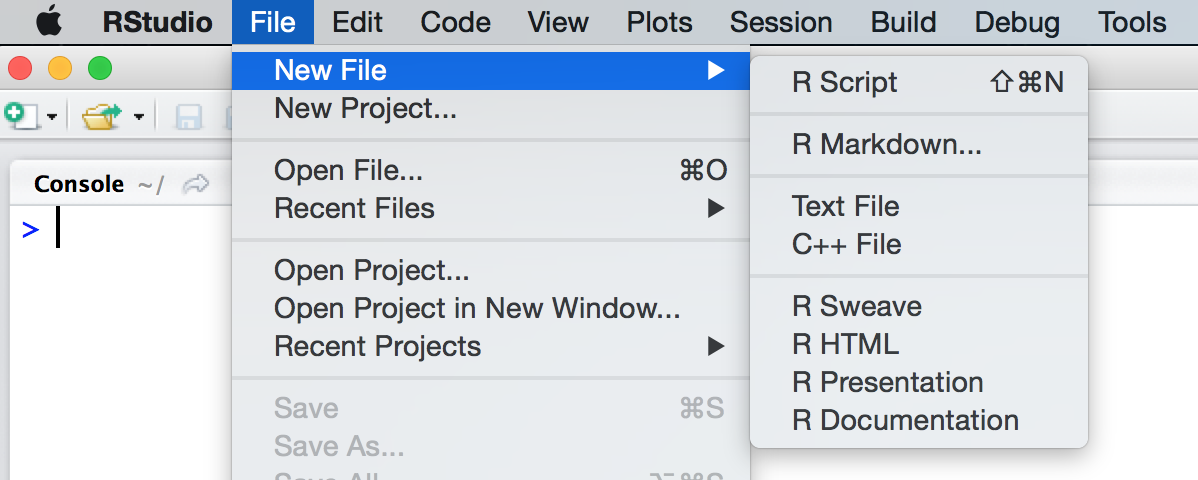
\includegraphics{figures/rstudio_newfile.png}
\caption{Tworzenie nowego skryptu R w interfejsie programu
\textbf{RStudio}}
\end{figure}

Lewe okno programu \textbf{RStudio} powinno podzielić się na 2 mniejsze,
z dotychczasowym terminalem na dole i nowym oknem do wpisywania skryptu
u góry.

Plik skryptowy R jest zwykłym plikiem tekstowym z rozszerzeniem
\texttt{.r} lub \texttt{.R}. Określenie ``zwykły plik tekstowy''
oznacza, że zawiera on tylko te informacje, które są widoczne na
ekranie. To trochę tak, jakby wszystkie nasze dotychczasowe komendy
wpisywane w terminalu zapisać w ``notatniku'', a następnie wklejać je w
zależności od potrzeb do terminala.

\subsection*{Jak działa skrypt R?}\label{jak-dziaa-skrypt-r}
\addcontentsline{toc}{subsection}{Jak działa skrypt R?}

Aby ``przenieść'' daną linię kodu z okna skryptowego do terminala i ją
wykonać należy posłużyć się skrótem \texttt{ctrl+enter}. Wówczas aktywna
linia kodu zostanie przeniesiona do terminala i wykonana.

Jeśli chcemy jednorazowo uruchomić więcej niż 1 linię kodu (np. jedno
polecenie rozpisaliśmy w kilku liniach) możemy zaznaczyć je myszką (lub
za pomocą strzałek i \texttt{shift}), a następnie wykonać ten blok kodu
stosując skrót \texttt{ctrl+enter}. Częste stosowanie tego skrótu
sprawi, że część osób nazwie te zajęcia ``ctrl+enter'' ;)

Docelowo będziemy dążyć do postaci, w której cały stworzony skrypt
stanowi spójną całość i może być uruchomiony linia po linii od początku
do końca. Zamiast wielokrotnego wciskania \texttt{ctrl+enter} linia po
linii (lub zaznaczenia całego kodu i naciśnięcia \texttt{ctrl+enter})
można ten sam efekt uzyskać za pomocą ikony \texttt{Source} znajdującej
się w prawym górnym rogu okna skryptowego (skrót:
\texttt{ctrl+shift+s}). Jest to równoznaczne z użyciem funkcji
\texttt{source(nazwa\_naszego\_pliku\_skryptowego.R)}.

\section{Praca ze skryptem}\label{praca-ze-skryptem}

Praca ze skryptami wymaga wyrobienia pewnych nawyków, które pozwolą na
bardziej efektywne tworzenie kodu i przetwarzanie danych.

\subsection{Komentarze}\label{komentarze}

Komentarz to fragment kodu znajdujący się bezpośrednio po znaku
\texttt{\#}, który nie jest interpretowany przez komputer podczas
wykonywania danego polecenia. W środowisku \textbf{RStudio} najczęściej
po znaku komentarza zmienia się kolor składni dający do zrozumienia
użytkownikowi, że dalszy fragment kodu to właśnie komentarzem:

\begin{Shaded}
\begin{Highlighting}[]
\KeywordTok{length}\NormalTok{(}\OperatorTok{-}\DecValTok{5}\OperatorTok{:}\DecValTok{5}\NormalTok{) }\CommentTok{# funkcja "length" zwraca liczbę elementów / tu: długość ciągu liczbowego}
\end{Highlighting}
\end{Shaded}

\begin{verbatim}
## [1] 11
\end{verbatim}

Dobrym zwyczajem, zwłaszcza na początku nauki programowania i/lub
przetwarzania danych jest tworzenie możliwie obszernych i precyzyjnych
komentarzy ułatwiających zrozumienie naszego działania lub
poszczególnych bloków kodu.

Jedna ze szkół programowania zakłada, że ``\emph{z komentarzy powinno
się móc wywnioskować wszystko co program robi, bez oglądania reszty
źródeł}'' \citep{dewhurst1995}. Stosowanie tej zasady pozwoli na dużą
oszczędność czasu, zwłaszcza jeśli nasz skrypt:

\begin{itemize}
\tightlist
\item
  jest używany do nauki programowania/przetwarzania danych,
\item
  jest stosunkowo skomplikowany,
\item
  zawiera wiele nowych elementów,
\item
  jest otwierany stosunkowo rzadko,
\item
  ma być docelowo używany także przez inne osoby.
\end{itemize}

Komentarze warto stosować także w odniesieniu do pewnych fragmentów
testowanego kodu, które chcemy chwilowo wyłączyć, ale nie chcemy się ich
na stałe pozbywać. Twórcy \textbf{RStudio} pomyśleli o takim
zastosowaniu dając użytkownikom skrót \texttt{ctrl+shift+c}, który w
zaznaczonym fragmencie kodu na początku każdej linii tworzy znak
komentarza. W celu przetestowania tego rozwiązania stwórz poniższy
fragment kodu nawiązujący do przeliczeń temperatury powietrza z stopni
Celsjusza na stopnie Fahrenheita:

\begin{Shaded}
\begin{Highlighting}[]
\NormalTok{tc <-}\StringTok{ }\DecValTok{-20} \CommentTok{# wartosc temperatury w *C }
\NormalTok{tf <-}\StringTok{ }\NormalTok{tc}\OperatorTok{*}\FloatTok{1.8}\OperatorTok{+}\DecValTok{32} \CommentTok{# przeliczamy na stopnie F}
\KeywordTok{print}\NormalTok{(tf) }\CommentTok{# wyświetlamy zawartość zmiennej tf}

\NormalTok{tc <-}\StringTok{ }\DecValTok{-10}\OperatorTok{:}\DecValTok{10} \CommentTok{# za drugim razem chcemy przetestowac zakres wartosci temperatury w *C od -10 do +10}
\NormalTok{tf <-}\StringTok{ }\NormalTok{tc}\OperatorTok{*}\FloatTok{1.8}\OperatorTok{+}\DecValTok{32} \CommentTok{# znowu przeliczamy na stopnie F}
\KeywordTok{print}\NormalTok{(tf) }\CommentTok{# wyświetlamy zawartość zmiennej tf}
\end{Highlighting}
\end{Shaded}

A następnie zaznacz ostatnie 3 linie kodu i zakomentuj skrótem
\texttt{ctrl+shift+c}. Uruchom cały kod (łącznie z zakomentowanymi
liniami) i dla pewności sprawdź wartości przechowywane w zmiennych.

\section{Wektory i podstawowe operacje na
wektorach}\label{wektory-i-podstawowe-operacje-na-wektorach}

Podstawowym typem obiektu w \textbf{R} są wektory. Znasz je już z
poprzednich ćwiczeń, kiedy traktowaliśmy \textbf{R} jako kalkulator, gdy
definiowaliśmy nowe obiekty lub generowaliśmy ciągi liczb. Nawet
pojedyncza wartość w \textbf{R} jest w rzeczywistości wektorem
(1-elementowym), natomiast jeśli chcemy dowolne operacje wykonywać na
większej liczbie elementów wówczas musimy te obiekty złączyć za pomocą
funkcji \texttt{c()}.

Warto zaznajomić się z podstawowym cechami pracy na wektorach w celu
uniknięcia późniejszych błędów.

\textbf{Zadanie}

\begin{enumerate}
\def\labelenumi{\arabic{enumi}.}
\tightlist
\item
  Stwórz wektor \texttt{x} o wartościach 0, 3, 2, 10, 5 oraz wektor
  \texttt{y} o wartościach 3, 4, 5. Wykonując operację dodawania,
  mnożenia i potęgowania na tych dwóch obiektach sprawdź jak działa
  \emph{autoreplikacja} w \textbf{R}.
\item
  Zmodyfikuj obiekt \texttt{y} tak aby zawierał tyle elementów co
  zmienna \texttt{x}, ale jako 4-ty i 5-ty element wprowadź wartości
  \texttt{NA} oznaczające brak danych. Ponownie przetestuj mnożenie na
  tych dwóch obiektach i sprawdź działanie autoreplikacji.
\item
  Przetestuj działanie funkcji \texttt{mean()} oraz \texttt{sum()} i
  \texttt{cumsum()} na obiekcie \texttt{y}. Korzystając z pomocy
  systemowej sprawdź jak ``naprawić'' wynik, tak aby uwzględniał on przy
  obliczaniu tylko wartości liczbowe.
\item
  Sprawdź działanie funkcji \texttt{sort()} na zmiennej \texttt{x}.
\item
  Sprawdź działanie funkcji \texttt{rev()} na zmiennej \texttt{y}.
\end{enumerate}

\begin{quote}
Staraj się przyswoić możliwie wiele funkcji omówionych do tej pory. W
praktyce najczęściej stosuje się kilkadziesiąt słów kluczowych, które
pozwalają na rozwiązanie większości spotykanych problemów
obliczeniowych.
\end{quote}

\subsection{Typy danych wektorowych}\label{typy-danych-wektorowych}

W \textbf{R} wektory mogą przechowywać nie tylko liczby, ale także typy
danych czynnikowych, datę, czas oraz ciągi tekstowe i logiczne. Póki co
omówimy w dużym skrócie te 2 ostatnie, które przydadzą się w kolejnym
podpunkcie.

\subsubsection{Typ tekstowy}\label{typ-tekstowy}

Deklaracja typu tekstowego odbywa się poprzez wpisanie dowolnego
wyrażenia między znaki cudzysłowia \texttt{"\ "} lub w ciapkach
\texttt{\textquotesingle{}\ \textquotesingle{}}. Jeśli chcemy stworzyć
obiekt przechowujący pierwsze litery alfabetu możemy go zdefiniować w
następujący sposób:

\begin{Shaded}
\begin{Highlighting}[]
\KeywordTok{c}\NormalTok{(}\StringTok{"a"}\NormalTok{,}\StringTok{"b"}\NormalTok{,}\StringTok{"c"}\NormalTok{)}
\end{Highlighting}
\end{Shaded}

\begin{verbatim}
## [1] "a" "b" "c"
\end{verbatim}

Warto zwrócić uwagę, że jeśli będziemy próbowali złączyć obiekty o
różnych typach \textbf{R} domyślnie postara się je ``sprowadzić'' do
postaci najbardziej ogólnej, co często wymusza przekonwertowanie jednego
typu danych w inny:

\begin{Shaded}
\begin{Highlighting}[]
\KeywordTok{c}\NormalTok{(}\DecValTok{1}\OperatorTok{:}\DecValTok{5}\NormalTok{, }\StringTok{"0"}\NormalTok{, }\StringTok{"5"}\NormalTok{)}
\end{Highlighting}
\end{Shaded}

\begin{verbatim}
## [1] "1" "2" "3" "4" "5" "0" "5"
\end{verbatim}

W powyższym przykładzie można rozpoznać konwersję liczb do typu
tekstowego ponieważ wszystkie elementy \textbf{R} wydrukował w
cudzysłowiach.

\textbf{Wniosek: w wektorze możemy przechowywać TYLKO jeden typ danych!
}

\subsubsection{Typ logiczny}\label{typ-logiczny}

Wiele procedur przetwarzania danych wymaga sprawdzania warunków
logicznych, które mogą przyjmować wartości PRAWDA lub FAŁSZ. W
środowisku \textbf{R} te wartości są deklarowane za pomocą słów
\texttt{TRUE} lub \texttt{FALSE}, które można sprowadzić do skróconego
zapisu dużymi literami \texttt{T} i \texttt{F}.

\begin{Shaded}
\begin{Highlighting}[]
\KeywordTok{c}\NormalTok{(}\OtherTok{TRUE}\NormalTok{, }\OtherTok{FALSE}\NormalTok{, }\OtherTok{TRUE}\NormalTok{, }\OtherTok{FALSE}\NormalTok{) }\CommentTok{# pelne slowa}
\end{Highlighting}
\end{Shaded}

\begin{verbatim}
## [1]  TRUE FALSE  TRUE FALSE
\end{verbatim}

\begin{Shaded}
\begin{Highlighting}[]
\KeywordTok{c}\NormalTok{(T, F, T, F) }\CommentTok{# to samo, ale w skroconym zapisie}
\end{Highlighting}
\end{Shaded}

\begin{verbatim}
## [1]  TRUE FALSE  TRUE FALSE
\end{verbatim}

Ciekawą własnością typu logicznego jest to, że po sprowadzeniu do
wartości numerycznej (np. funkcją \texttt{as.numeric()}) przyjmuje ona
wartości 1 (prawda) lub 0 (fałsz):

\begin{Shaded}
\begin{Highlighting}[]
\NormalTok{logiczny <-}\StringTok{ }\KeywordTok{c}\NormalTok{(}\OtherTok{TRUE}\NormalTok{, }\OtherTok{FALSE}\NormalTok{) }
\KeywordTok{as.numeric}\NormalTok{(logiczny)}
\end{Highlighting}
\end{Shaded}

\begin{verbatim}
## [1] 1 0
\end{verbatim}

\subsection{Indeksowanie wektorów}\label{indeksowanie-wektorow}

Indeksowanie wektorów polega na wyborze określonych elementów obiektu
poprzez wskazanie ich pozycji. Indeksy wektora w \textbf{R} numerowane
są od 1 do n, gdzie n to długość (liczba elementów) wektora. Jeśli nie
znasz długości wektora zawsze możesz ją sprawdzić za pomocą funkcji
\texttt{length()}.

Wybór dowolnych elementów wektora jest możliwy przez zastosowanie
operatora \texttt{{[}{]}} wpisując jako argument pozycję, którą chcemy
pobrać. Na początek stwórzmy wektor zawierający 20 losowych liczb z
przedziału od 0 do 1. Nazwijmy ten obiekt \texttt{dane} i wyświetlmy
jego zawartość:

\begin{Shaded}
\begin{Highlighting}[]
\NormalTok{dane <-}\StringTok{ }\KeywordTok{runif}\NormalTok{(}\DecValTok{20}\NormalTok{)}
\NormalTok{dane}
\end{Highlighting}
\end{Shaded}

\begin{verbatim}
##  [1] 0.899049622 0.784734013 0.595490900 0.300648547 0.234256251
##  [6] 0.302369527 0.337933923 0.780297597 0.012236627 0.389173037
## [11] 0.762023591 0.549608661 0.857791153 0.259316680 0.857080017
## [16] 0.255409679 0.247717798 0.326963206 0.007979414 0.259561501
\end{verbatim}

Komenda pozwalająca na pobranie np. tylko piątego elementu:

\begin{Shaded}
\begin{Highlighting}[]
\NormalTok{dane[}\DecValTok{5}\NormalTok{]}
\end{Highlighting}
\end{Shaded}

\begin{verbatim}
## [1] 0.2342563
\end{verbatim}

Do wyświetlenia np. tylko pierwszych 10-ciu elementów musimy w nawiasie
kwadratowym wprowadzić numery indeksów od 1 do 10. Wymaga to
wygenerowania ciągu liczb, który będzie traktowany przez \textbf{R} jako
ciąg liczb 1, 2, 3, 4, 5, 6, 7, 8, 9, 10. Można ten efekt osiągnąć
przynajmnie na 2 sposoby.

\begin{enumerate}
\def\labelenumi{\arabic{enumi}.}
\tightlist
\item
  Poprzez konkatenację \texttt{c()}:
\end{enumerate}

\begin{Shaded}
\begin{Highlighting}[]
\NormalTok{dane[ }\KeywordTok{c}\NormalTok{(}\DecValTok{1}\NormalTok{,}\DecValTok{2}\NormalTok{,}\DecValTok{3}\NormalTok{,}\DecValTok{4}\NormalTok{,}\DecValTok{5}\NormalTok{,}\DecValTok{6}\NormalTok{,}\DecValTok{7}\NormalTok{,}\DecValTok{8}\NormalTok{,}\DecValTok{9}\NormalTok{,}\DecValTok{10}\NormalTok{) ]}
\end{Highlighting}
\end{Shaded}

\begin{verbatim}
##  [1] 0.89904962 0.78473401 0.59549090 0.30064855 0.23425625 0.30236953
##  [7] 0.33793392 0.78029760 0.01223663 0.38917304
\end{verbatim}

\begin{enumerate}
\def\labelenumi{\arabic{enumi}.}
\setcounter{enumi}{1}
\tightlist
\item
  Poprzez stworzenie ciągu liczb za pomocą operatora \texttt{:}
\end{enumerate}

\begin{Shaded}
\begin{Highlighting}[]
\NormalTok{dane[ }\DecValTok{1}\OperatorTok{:}\DecValTok{10}\NormalTok{ ]}
\end{Highlighting}
\end{Shaded}

\begin{verbatim}
##  [1] 0.89904962 0.78473401 0.59549090 0.30064855 0.23425625 0.30236953
##  [7] 0.33793392 0.78029760 0.01223663 0.38917304
\end{verbatim}

W analogiczny sposób możemy także odwrócić kolejność elementów obiektu
\texttt{dane} wyświetlając zbiór wartości malejących od 20 do 1 z
interwałem co 1:

\begin{Shaded}
\begin{Highlighting}[]
\NormalTok{dane[}\DecValTok{20}\OperatorTok{:}\DecValTok{1}\NormalTok{]}
\end{Highlighting}
\end{Shaded}

\begin{verbatim}
##  [1] 0.259561501 0.007979414 0.326963206 0.247717798 0.255409679
##  [6] 0.857080017 0.259316680 0.857791153 0.549608661 0.762023591
## [11] 0.389173037 0.012236627 0.780297597 0.337933923 0.302369527
## [16] 0.234256251 0.300648547 0.595490900 0.784734013 0.899049622
\end{verbatim}

Możemy także spróbować wyświetlić tylko wskazane przez nas indeksy.
Jeśli chcemy wyświetlić 2 razy 10-ty element, następnie 2-gi, a potem
19-ty to możemy ponownie wykorzystać funkcję \texttt{c()}, która pozwala
na stworzenie wektora składającego się z dowolnej konfiguracji indeksów.

\begin{Shaded}
\begin{Highlighting}[]
\NormalTok{dane[ }\KeywordTok{c}\NormalTok{(}\DecValTok{10}\NormalTok{,}\DecValTok{10}\NormalTok{,}\DecValTok{2}\NormalTok{,}\DecValTok{19}\NormalTok{) ]}
\end{Highlighting}
\end{Shaded}

\begin{verbatim}
## [1] 0.389173037 0.389173037 0.784734013 0.007979414
\end{verbatim}

\begin{quote}
W indeksowaniu ważne jest aby wyrażenie znajdujące się w \texttt{{[}{]}}
było wektorem! Jeśli nie nabrałeś jeszcze wprawy w tworzeniu wektorów za
pomocą \texttt{c()} oraz \texttt{:} zawsze możesz przetestować roboczo
działanie wprowadzanego wyrażenia indeksującego w konsoli
\end{quote}

W praktyce często do indeksowania wykorzystuje się inne obiekty
(wektory), które zawierają numery pozycji do pobrania. Sprawdźmy to na
przykładzie:

\begin{Shaded}
\begin{Highlighting}[]
\NormalTok{indeks <-}\StringTok{ }\KeywordTok{c}\NormalTok{(}\DecValTok{1}\NormalTok{,}\DecValTok{5}\NormalTok{,}\DecValTok{10}\NormalTok{) }\CommentTok{# tworzymy wektor wartości 1, 5, 10}
\NormalTok{dane[indeks] }\CommentTok{# wyswietlamy wskazane numery, ktore sa przechowywane w obiekcie `indeks`}
\end{Highlighting}
\end{Shaded}

\begin{verbatim}
## [1] 0.8990496 0.2342563 0.3891730
\end{verbatim}

\subsubsection{\texorpdfstring{Indeksowanie przez
``negację''}{Indeksowanie przez negację}}\label{indeksowanie-przez-negacje}

Ciekawym rozwiązaniem pozwalającym w wielu przypadkach na pozbycie się
niechcianych elementów jest zastosowanie jako indeksu liczb ujemnych.
Jeśli chcemy pozbyć się tylko np. pierwszego elementu z naszego obiektu
(np. zawiera błąd), wówczas zamiast wpisywać komendę
\texttt{dane{[}2:19{]}} możemy ten sam efekt osiągnąć stosując poniższy
zapis:

\begin{Shaded}
\begin{Highlighting}[]
\NormalTok{dane[}\OperatorTok{-}\DecValTok{1}\NormalTok{]}
\end{Highlighting}
\end{Shaded}

\begin{verbatim}
##  [1] 0.784734013 0.595490900 0.300648547 0.234256251 0.302369527
##  [6] 0.337933923 0.780297597 0.012236627 0.389173037 0.762023591
## [11] 0.549608661 0.857791153 0.259316680 0.857080017 0.255409679
## [16] 0.247717798 0.326963206 0.007979414 0.259561501
\end{verbatim}

Wybór poprzez eliminację nie musi się ograniczać do pojedynczego
indeksu. Możliwe jest także stworzenie wektora dowolnych liczb ujemnych:

\begin{Shaded}
\begin{Highlighting}[]
\NormalTok{dane[}\KeywordTok{c}\NormalTok{(}\OperatorTok{-}\DecValTok{1}\NormalTok{,}\OperatorTok{-}\DecValTok{20}\NormalTok{)] }\CommentTok{# pozbywamy sie pierwszego i ostatniego elementu}
\end{Highlighting}
\end{Shaded}

\begin{verbatim}
##  [1] 0.784734013 0.595490900 0.300648547 0.234256251 0.302369527
##  [6] 0.337933923 0.780297597 0.012236627 0.389173037 0.762023591
## [11] 0.549608661 0.857791153 0.259316680 0.857080017 0.255409679
## [16] 0.247717798 0.326963206 0.007979414
\end{verbatim}

\begin{Shaded}
\begin{Highlighting}[]
\NormalTok{dane[}\KeywordTok{c}\NormalTok{(}\OperatorTok{-}\DecValTok{5}\OperatorTok{:-}\DecValTok{10}\NormalTok{, }\DecValTok{-15}\OperatorTok{:-}\DecValTok{20}\NormalTok{) ] }\CommentTok{# pozbywamy sie elementow od 5. do 10. oraz od 15. do 20.}
\end{Highlighting}
\end{Shaded}

\begin{verbatim}
## [1] 0.8990496 0.7847340 0.5954909 0.3006485 0.7620236 0.5496087 0.8577912
## [8] 0.2593167
\end{verbatim}

\subsubsection{Indeksowanie za pomocą wyrażeń
logicznych}\label{indeksowanie-za-pomoca-wyrazen-logicznych}

Ciekawym rozwiązaniem przy indeksowaniu może być zastosowanie wartości
logicznych \texttt{TRUE} lub \texttt{FALSE}. Na początek stwórzmy nowy
wektor zawierający nazwy 4-ech losowych miast i nazwijmy go
\texttt{miasta}.

\begin{Shaded}
\begin{Highlighting}[]
\NormalTok{miasta <-}\StringTok{ }\KeywordTok{c}\NormalTok{(}\StringTok{"Poznań"}\NormalTok{, }\StringTok{"Wrocław"}\NormalTok{, }\StringTok{"Warszawa"}\NormalTok{, }\StringTok{"Kraków")}
\end{Highlighting}
\end{Shaded}

Stosując wektor logiczny o wartościach \texttt{TRUE} lub \texttt{FALSE}
możemy indeksować, które elementy mają zostać pobrane:

\begin{Shaded}
\begin{Highlighting}[]
\NormalTok{miasta[}\KeywordTok{c}\NormalTok{(}\OtherTok{TRUE}\NormalTok{, }\OtherTok{TRUE}\NormalTok{, }\OtherTok{FALSE}\NormalTok{, }\OtherTok{TRUE}\NormalTok{)]}
\end{Highlighting}
\end{Shaded}

\begin{verbatim}
## [1] "Poznań"  "Wrocław" "Kraków"
\end{verbatim}

\section{Indeksowanie z użyciem warunków
logicznych}\label{indeksowanie-z-uzyciem-warunkow-logicznych}

Indeksowanie jest niezmiernie ważnym elementem pracy z danymi w
\textbf{R}. Szybkie i efektywne przetwarzenie danych wymaga testowania
warunków logicznych (o tym szerzej w kolejnych częściach kursu), które
pozwalają na odfiltrowanie zbiorów danych na których chcemy wykonać
naszą analizę. Najczęściej sprowadza się to do stworzenia nowych
obiektów (wektorów) przechowujących numery pozycji lub wartości logiczne
spełniające dany test. Poniżej zamieszczono tabelę z podstawowymi
operacjami logicznymi w \textbf{R}:

\begin{longtable}[]{@{}ll@{}}
\caption{Podstawowe operatory logiczne w \textbf{R}}\tabularnewline
\toprule
Operator & Działanie operatora\tabularnewline
\midrule
\endfirsthead
\toprule
Operator & Działanie operatora\tabularnewline
\midrule
\endhead
\texttt{\textless{}} & mniejsze od\tabularnewline
\texttt{\textless{}=} & mniejsze bądź równe\tabularnewline
\texttt{\textgreater{}} & większe od\tabularnewline
\texttt{\textgreater{}=} & większe bądź równe\tabularnewline
\texttt{==} & równe\tabularnewline
\texttt{!=} & różne od\tabularnewline
\texttt{!x} & negacja\tabularnewline
\texttt{x\ \textbar{}\ y} & suma logiczna zbiorów\tabularnewline
\texttt{x\ \&\ y} & iloczyn logiczny zbiorów\tabularnewline
\bottomrule
\end{longtable}

\subsection{Testowanie warunków
logicznych}\label{testowanie-warunkow-logicznych}

Działanie operatorów logicznych najlepiej sprawdzić w praktyce. Na
początek stwórzmy obiekt \texttt{dane2}, w którym będziemy przechowywać
30 losowych wartości od -1 do +1 i wyświetlmy jego zawartość

\begin{Shaded}
\begin{Highlighting}[]
\NormalTok{dane2 <-}\StringTok{ }\KeywordTok{runif}\NormalTok{(}\DataTypeTok{n =} \DecValTok{30}\NormalTok{, }\DataTypeTok{min =} \DecValTok{-1}\NormalTok{, }\DataTypeTok{max =} \DecValTok{1}\NormalTok{)}
\NormalTok{dane2}
\end{Highlighting}
\end{Shaded}

\begin{verbatim}
##  [1]  0.18754995  0.37016365  0.39507023  0.91508907 -0.53614377
##  [6]  0.25714506  0.82342568  0.55519429 -0.12100064 -0.23853956
## [11] -0.68655516  0.98477907  0.17569978 -0.61603732  0.79882611
## [16] -0.54385309  0.88125978 -0.70620560 -0.39978640 -0.12945671
## [21] -0.53897525  0.28954366  0.66643144 -0.09009203  0.57269675
## [26]  0.04207847 -0.29460512  0.06032883 -0.05954098  0.21969730
\end{verbatim}

Sprawdzenie, które liczby są większe bądź równe 0 jest możliwe poprzez
zastosowanie komendy:

\begin{Shaded}
\begin{Highlighting}[]
\NormalTok{dane2 }\OperatorTok{>=}\StringTok{ }\DecValTok{0}
\end{Highlighting}
\end{Shaded}

\begin{verbatim}
##  [1]  TRUE  TRUE  TRUE  TRUE FALSE  TRUE  TRUE  TRUE FALSE FALSE FALSE
## [12]  TRUE  TRUE FALSE  TRUE FALSE  TRUE FALSE FALSE FALSE FALSE  TRUE
## [23]  TRUE FALSE  TRUE  TRUE FALSE  TRUE FALSE  TRUE
\end{verbatim}

Otrzymany wynik 30-tu wartości (\texttt{TRUE/FALSE}) wskazuje czy w
danym indeksie wartość spełnia dany warunek logiczny. Jeśli chcemy się
pozbyć wartości ujemnych możemy np. stworzyć wektor wartości logicznych,
zapisać go jako nowy obiekt i podstawić jako indeks:

\begin{Shaded}
\begin{Highlighting}[]
\NormalTok{indeks <-}\StringTok{  }\NormalTok{dane2 }\OperatorTok{>=}\StringTok{ }\DecValTok{0}        \CommentTok{#   tworzymy wektor indeksujacy}
\NormalTok{dane2 [ indeks ]}
\end{Highlighting}
\end{Shaded}

\begin{verbatim}
##  [1] 0.18754995 0.37016365 0.39507023 0.91508907 0.25714506 0.82342568
##  [7] 0.55519429 0.98477907 0.17569978 0.79882611 0.88125978 0.28954366
## [13] 0.66643144 0.57269675 0.04207847 0.06032883 0.21969730
\end{verbatim}

Lub z pominięciem etapu tworzenia tymczasowego obiektu indeksującego:

\begin{Shaded}
\begin{Highlighting}[]
\NormalTok{dane2 [ dane2 }\OperatorTok{>=}\StringTok{ }\DecValTok{0}\NormalTok{ ]}
\end{Highlighting}
\end{Shaded}

\begin{verbatim}
##  [1] 0.18754995 0.37016365 0.39507023 0.91508907 0.25714506 0.82342568
##  [7] 0.55519429 0.98477907 0.17569978 0.79882611 0.88125978 0.28954366
## [13] 0.66643144 0.57269675 0.04207847 0.06032883 0.21969730
\end{verbatim}

\subsection{\texorpdfstring{Funkcja
\emph{which}}{Funkcja which}}\label{funkcja-which}

W wielu przypadkach bardziej wygodna w użyciu będzie funkcja
\texttt{which()} (ang. \emph{``który''}) zwracająca numery pozycji
spełniających dany warunek logiczny.

\begin{quote}
\texttt{which()} (ang. \emph{``który/które''}) - czyli które elementy
spełniają dany warunek logiczny.
\end{quote}

Poniższa komenda wskazuje indeksy wektora \texttt{dane2} większe od 0

\begin{Shaded}
\begin{Highlighting}[]
\KeywordTok{which}\NormalTok{(dane2}\OperatorTok{>}\DecValTok{0}\NormalTok{)}
\end{Highlighting}
\end{Shaded}

\begin{verbatim}
##  [1]  1  2  3  4  6  7  8 12 13 15 17 22 23 25 26 28 30
\end{verbatim}

Możemy także jednorazowo wykonać 2 testy logiczne, takby aby wybrać np.
liczby które są jednocześnie większe bądź równe -0.5 i mniejsze bądź
równe -0.1. Graficznie taką zależność możemy wyobrazić sobie jako
znalezienie elementów, które zawierają się w niebieskim prostokącie.

\begin{verbatim}
## Warning in title(...): conversion failure on 'wartości obiektu dane2' in
## 'mbcsToSbcs': dot substituted for <c5>
\end{verbatim}

\begin{verbatim}
## Warning in title(...): conversion failure on 'wartości obiektu dane2' in
## 'mbcsToSbcs': dot substituted for <9b>
\end{verbatim}

\begin{figure}

{\centering 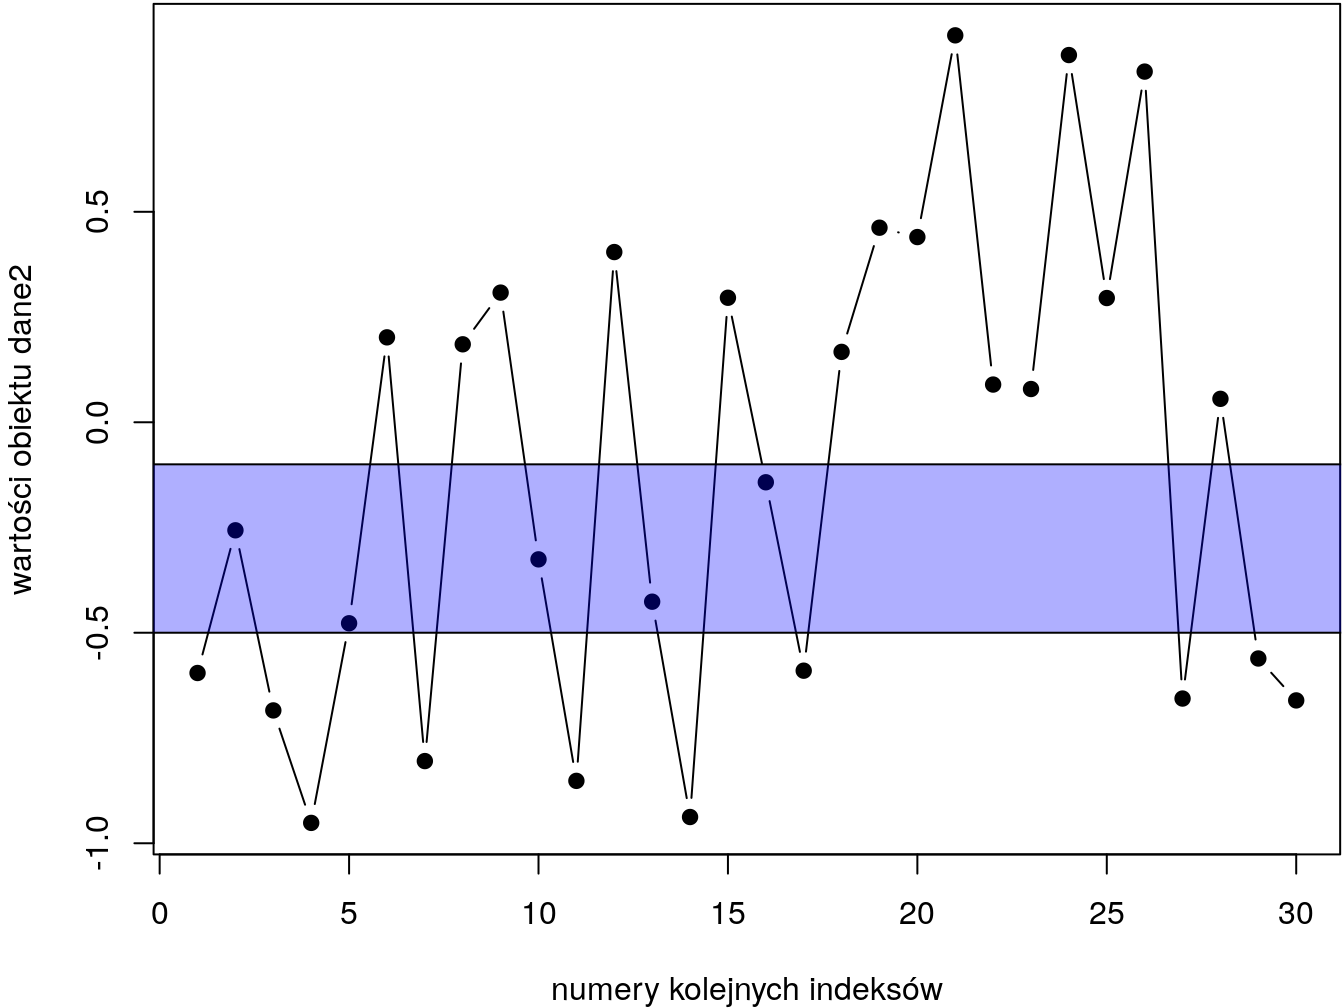
\includegraphics[width=0.8\linewidth]{ksiazka_files/figure-latex/przyklad-1} 

}

\caption{Znajdowanie liczb znajdujących się w przedziale domkniętym od -0.5 od -0.1.}\label{fig:przyklad}
\end{figure}

Odszukanie indeksów tych elementów w składni \textbf{R} jest możliwe z
wykorzystaniem wyrażeń logicznych i funkcji \texttt{which()}

\begin{Shaded}
\begin{Highlighting}[]
\KeywordTok{which}\NormalTok{(dane2 }\OperatorTok{>=}\StringTok{ }\FloatTok{-0.5} \OperatorTok{&}\StringTok{ }\NormalTok{dane2 }\OperatorTok{<=}\StringTok{ }\FloatTok{-0.1}\NormalTok{ )}
\end{Highlighting}
\end{Shaded}

\begin{verbatim}
## [1]  9 10 19 20 27
\end{verbatim}

Operator \texttt{\&} oznacza iloczyn logiczny zbioru. Jeśli
interesowałyby nas wartości, które są jednocześnie mniejsze od -0.5
LUBsą większe od 0.5 (jak na rys. \ref{fig:przyklad2} ), wówczas zamiast
iloczynu logicznego powinniśmy użyć sumy logicznej zbioru (czyli
operatora \texttt{\textbar{}}).

\begin{verbatim}
## Warning in title(...): conversion failure on 'wartości obiektu dane2' in
## 'mbcsToSbcs': dot substituted for <c5>
\end{verbatim}

\begin{verbatim}
## Warning in title(...): conversion failure on 'wartości obiektu dane2' in
## 'mbcsToSbcs': dot substituted for <9b>
\end{verbatim}

\begin{figure}

{\centering 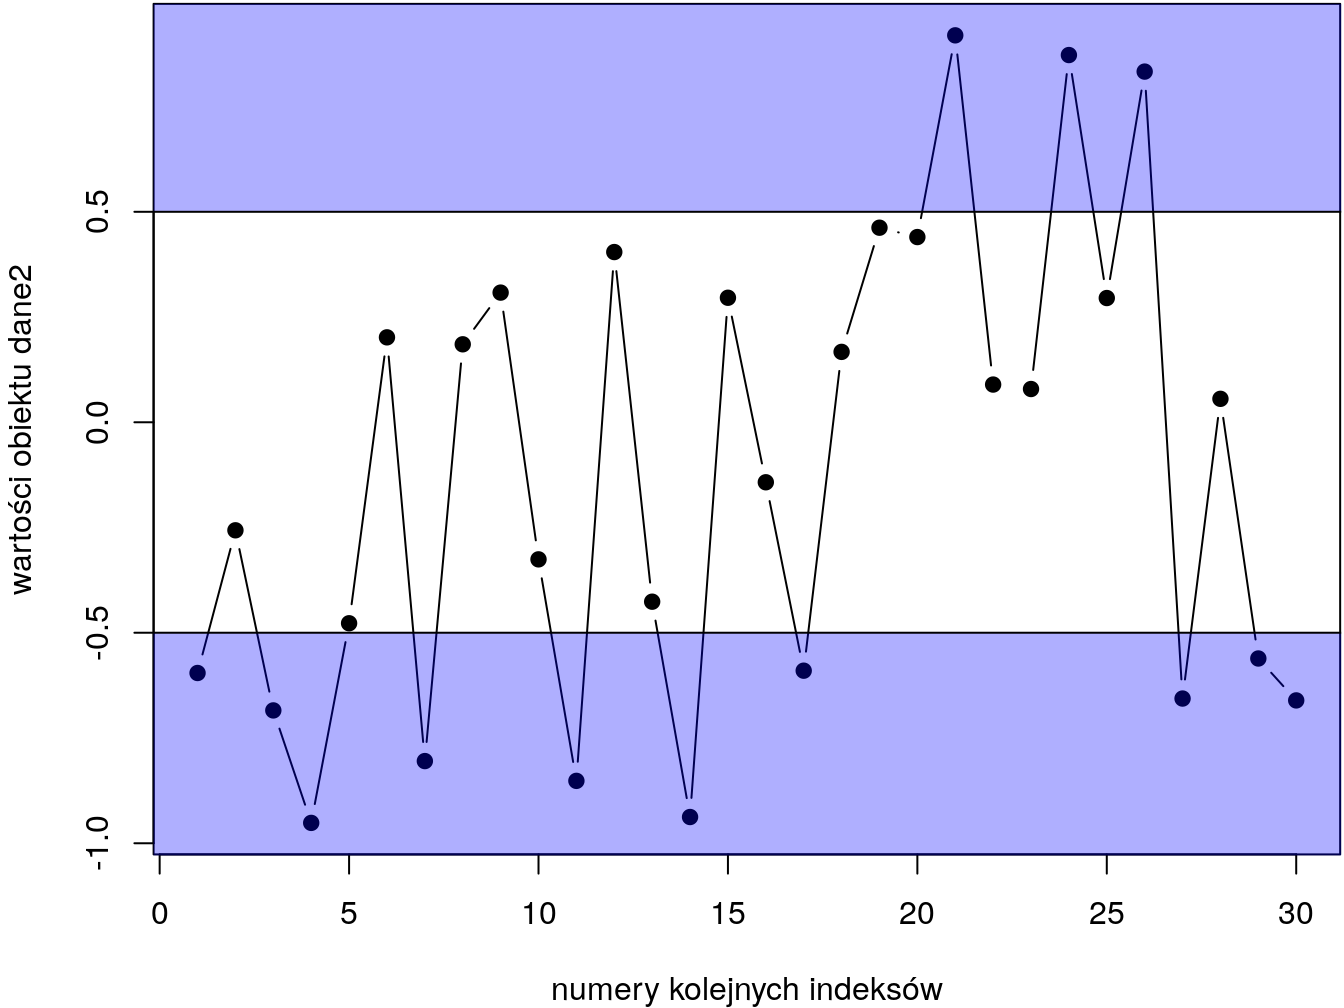
\includegraphics[width=0.8\linewidth]{ksiazka_files/figure-latex/przyklad2-1} 

}

\caption{Znajdowanie wartości mniejszych od -0.5 i większych od 0.5}\label{fig:przyklad2}
\end{figure}

\begin{Shaded}
\begin{Highlighting}[]
\KeywordTok{which}\NormalTok{(dane2}\OperatorTok{<}\StringTok{ }\FloatTok{-0.5} \OperatorTok{|}\StringTok{ }\NormalTok{dane2}\OperatorTok{>}\StringTok{ }\FloatTok{0.5}\NormalTok{)}
\end{Highlighting}
\end{Shaded}

\begin{verbatim}
##  [1]  4  5  7  8 11 12 14 15 16 17 18 21 23 25
\end{verbatim}

Jeśli interesują nas same wartości spełniające dany warunek logiczny (a
nie indeksy) możemy zapisać wynik powyższego działania do nowego obiektu
i wykorzystać go jako wektor indeksujący

\begin{Shaded}
\begin{Highlighting}[]
\NormalTok{indeks <-}\StringTok{ }\KeywordTok{which}\NormalTok{(dane2}\OperatorTok{<}\StringTok{ }\FloatTok{-0.5} \OperatorTok{|}\StringTok{ }\NormalTok{dane2}\OperatorTok{>}\StringTok{ }\FloatTok{0.5}\NormalTok{)}
\NormalTok{dane2[indeks]}
\end{Highlighting}
\end{Shaded}

\begin{verbatim}
##  [1]  0.9150891 -0.5361438  0.8234257  0.5551943 -0.6865552  0.9847791
##  [7] -0.6160373  0.7988261 -0.5438531  0.8812598 -0.7062056 -0.5389752
## [13]  0.6664314  0.5726967
\end{verbatim}

Jeśli chcemy wyświetlić wszystkie pozostałe wartości możemy postawić
znak minus w \texttt{{[}{]}} , co da nam wartości indeksu pomnożone razy
-1

\begin{Shaded}
\begin{Highlighting}[]
\NormalTok{dane2[}\OperatorTok{-}\NormalTok{indeks] }\CommentTok{# lub to samo zapisane jako: dane2[indeks * -1]}
\end{Highlighting}
\end{Shaded}

\begin{verbatim}
##  [1]  0.18754995  0.37016365  0.39507023  0.25714506 -0.12100064
##  [6] -0.23853956  0.17569978 -0.39978640 -0.12945671  0.28954366
## [11] -0.09009203  0.04207847 -0.29460512  0.06032883 -0.05954098
## [16]  0.21969730
\end{verbatim}

\section{Zadania podsumowujące}\label{zadania-podsumowujace}

\subsection{Skrypt}\label{skrypt}

\begin{enumerate}
\def\labelenumi{\arabic{enumi}.}
\item
  Utwórz nowy skrypt i skopiuj do niego zawartość kodu ze strony:
  {[}\url{http://enwo.pl/przetwarzanie/lorenz.r}{]}
  (\url{http://enwo.pl/przetwarzanie/lorenz.r})
\item
  Uruchom skrypt
\end{enumerate}

\subsection{Tworzenie wektorów}\label{tworzenie-wektorow}

\begin{enumerate}
\def\labelenumi{\arabic{enumi}.}
\item
  Stwórz wektor \texttt{miasta} składający z 3-ech losowych nazw
  miejscowości.
\item
  Dołącz do obiektu \texttt{miasta} kolejne o nazwie \emph{Wzdół
  Rządowy}
  {[}\href{https://pl.wikipedia.org/wiki/Wzd\%C3\%B3\%C5\%82_Rz\%C4\%85dowy}{1}{]},
  {[}\href{http://www.tvp.info/2514948/po-godzinach/bialy-kal-zniknal-suchecipki-zostaja/}{2}
  {]}.
\item
  Nadpisz zawartość wektora \texttt{miasta} usuwając ostatnią nazwę,
  gdyż \emph{Wzdół Rządowy} jest wsią a nie miastem.
\end{enumerate}

\subsection{Indeksowanie}\label{indeksowanie}

\begin{enumerate}
\def\labelenumi{\arabic{enumi}.}
\item
  Wyświetl zawartość wbudowanej zmiennej \texttt{letters}
\item
  Jaka jest 24-ta litera alfabetu zapisanego w obiekcie
  \texttt{letters}?
\item
  Ile liter jest dalej w alfabecie niż litera \texttt{s} ? Wykorzystaj
  zapytanie logiczne \texttt{\textgreater{}}
\end{enumerate}

\begin{quote}
Przydatna może być także wiedza o wartościach numerycznych dla
\texttt{TRUE/FALSE} oraz funkcji \texttt{sum()}.
\end{quote}

\begin{enumerate}
\def\labelenumi{\arabic{enumi}.}
\setcounter{enumi}{3}
\tightlist
\item
  Korzystając z operatora \texttt{{[}{]}} wyświetl:
\end{enumerate}

\begin{enumerate}
\def\labelenumi{\alph{enumi})}
\tightlist
\item
  parzyste litery alfabetu (2,4,6 \ldots{})
\item
  nieparzyste litery alfabetu (1,3,5 \ldots{})
\end{enumerate}

\begin{center}\rule{0.5\linewidth}{\linethickness}\end{center}

5.1. Stwórz obiekty \texttt{lon} i \texttt{lat} zawierające wartości
południków (\texttt{lon}) i równoleżników (\texttt{lat}) dla obszaru
Europy odpowiadającej siatce modelu GFS. Model GFS ma rozdzielczość
przestrzenną 0.25 x 0.25 stopnia. Przyjmij roboczo, że obszar Europy
zawiera się w od 25W do 40E oraz od 30N do 75N (rys. \ref{fig:mapagfs}
). Dla oznaczenia długości geograficznej przyjmij wartości ujemne dla
długości geograficznej zachodniej (tj. 25W = -25) i dodatnie dla
długości geograficznej wschodniej (tj. 40E = 40). Kontrolnie możesz
sprawdzić długość powstałych obiektów (funkcją \texttt{length()}).
Sprawdź czy stworzono 261 południków i 181 równoleżników.

\begin{figure}

{\centering 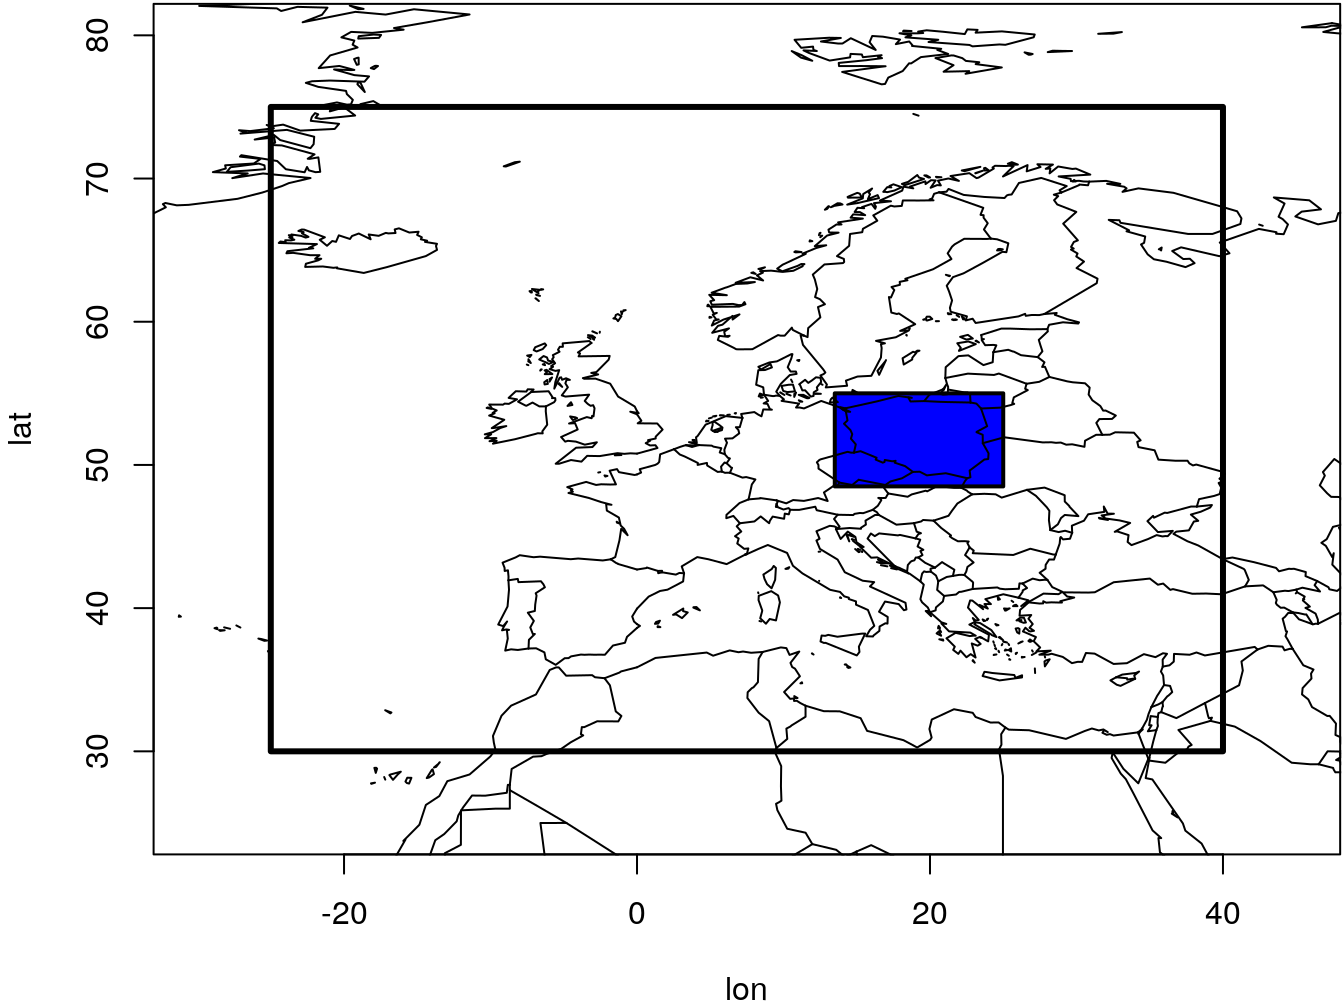
\includegraphics[width=0.8\linewidth]{ksiazka_files/figure-latex/mapagfs-1} 

}

\caption{Schemat domeny obliczeniowej modelu GFS dla Europy}\label{fig:mapagfs}
\end{figure}

5.2. Za pomocą funkcji \texttt{which()} wskaż numery indeksów
\texttt{lon} i \texttt{lat}, które zawierają obszar Polski
(\ref{fig:mapagfs} ). Przyjmij roboczo, że długości geograficzne powinny
zawierać się w przedziale od 13.5 do 25, a szerokości od 48.5 do 55.

5.3. Z obiektów \texttt{lon} i \texttt{lat} wydobądź poprzez operator
\texttt{{[}\ {]}} wartości południków i równoleżników w podanym powyżej
zakresie (13.5E-25.0E, 48.5N-55.0N). Wartości zapisz do nowych obiektów
\texttt{lon2} i \texttt{lat2}.

5.4. Ile elementów zawierają nowe obiekty \texttt{lon2} i \texttt{lat2}
?

\begin{center}\rule{0.5\linewidth}{\linethickness}\end{center}

\section*{Zadanie domowe}\label{zadanie-domowe}
\addcontentsline{toc}{section}{Zadanie domowe}

\begin{enumerate}
\def\labelenumi{\arabic{enumi}.}
\tightlist
\item
  Korzystając z wbudowanego systemu pomocy puść ``totolotka'' za pomocą
  funkcji \texttt{sample()} generując zestaw liczb od 1 do 49, a
  następnie wywołując parametr \texttt{size=} dla sześciu liczb.
\item
  Wygeneruj i zapisz w postaci wektora dowolny ciąg liczbowy składający
  się z 20-50 liczb. Następnie korzystając z wygenerowanych liczb i
  wbudowanego systemu pomocy przetestuj działanie poniższych funkcji:
\end{enumerate}

\begin{longtable}[]{@{}ll@{}}
\caption{Wybrane funkcje uzupełniające niezbędną wiedzę do pracy na
wektorach w \textbf{R}}\tabularnewline
\toprule
Nazwa funkcji & Działanie\tabularnewline
\midrule
\endfirsthead
\toprule
Nazwa funkcji & Działanie\tabularnewline
\midrule
\endhead
\texttt{summary()} & statystyki podsumowujące\tabularnewline
\texttt{range()} & zwraca jednocześnie minimalną i maksymalną
wartość\tabularnewline
\texttt{rev()} & odwraca kolejność elementów\tabularnewline
\texttt{rep()} & replikacja / powtarzanie /
zwielokrotnienie\tabularnewline
\texttt{sort()} & sortowanie\tabularnewline
\texttt{length()} & długość obiektu\tabularnewline
\bottomrule
\end{longtable}

\begin{center}\rule{0.5\linewidth}{\linethickness}\end{center}

\section*{Zadania sprawdzające}\label{zadania-sprawdzajace-1}
\addcontentsline{toc}{section}{Zadania sprawdzające}

\url{https://goo.gl/forms/EMbuMMHVSIkQeP2q2}

\chapter{Ramki danych i macierze}\label{ramki-danych-i-macierze}

W poprzednim rozdziale omówiono kilka schematów posługiwania się
wektorami, który są jednocześnie najbardziej elementarnym sposobem
przetwarzania danych w \textbf{R}.

\section{Ramki danych}\label{ramki-danych}

Przy analizie danych (w tym także danych meteorologicznych)
wykorzystywane są inne niż wektory schematy przechowywania i
przetwarzania danych. Najczęściej są to tzw. ramki danych (ang.
\emph{data frame}), które na pierwszy rzut oka przypominają tradycyjną
``tabelkę z Excela''.

Najważniejsze cechy ramki danych wypisano poniżej:

\begin{enumerate}
\def\labelenumi{\arabic{enumi}.}
\tightlist
\item
  Każda ramka danych powinna zawierać wartości uporządkowane w
  kolumnach.
\item
  Każda z kolumn jest wektorem i musi mieć taką samą długość.
\item
  Różne kolumny mogą przechowywać różne typy danych.
\end{enumerate}

Poniżej zamieszczono fragment ramki danych zawiera dane pomiarowe ze
stacji Wojewódzkiego Inspektoratu Ochrony Środowiska - Poznań-Polanka. W
kolumnie \emph{date} zawarto dane w typie umożliwiającym przechowywanie
czasu, w kolejnych kolumnach umieszczono wartości koncentracji PM10,
PM2.5, temperatury powietrza, prędkości wiatru o oraz kierunku wiatru.

\begin{verbatim}
##                      date PZ_Pol_pm10 PZ_Pol_pm25 PZ_T2M PZ_WS PZ_WD
## 95034 2016-11-07 17:00:00          24          16      4     1   278
## 95035 2016-11-07 18:00:00          22          17      4     1   287
## 95036 2016-11-07 19:00:00          22          17      3     1   322
## 95037 2016-11-07 20:00:00          23          16      3     1   326
## 95038 2016-11-07 21:00:00          24          16      3     0   307
## 95039 2016-11-07 22:00:00          24          16      2     0   303
\end{verbatim}

\section{Praca na ramkach danych}\label{praca-na-ramkach-danych}

Do nauki pracy na ramkach danych wykorzystamy domyślnie wgrane zbiór
danych o nazwie \emph{airquality}. Wczytanie przykładowego zbioru danych
wgranego wraz z \textbf{R} jest możliwe poprzez funkcję \texttt{data()}.
Nasz zbiór nazywa się \texttt{airquality}. Szczegóły dotyczące
analizowanego zbioru danych dostępne są po wydaniu komendy
\texttt{?airquality} lub \texttt{?"airquality"}

Jeśli chcemy wczytać i wyświetlić pierwsze kilka rzędów naszej ramki
danych spróbujmy najpierw ją wczytać do pamięci komputera a następnie
wyświetlić pierwsze lub ostatnie 6 wierszy za pomocą funkcji
\texttt{head()} lub \texttt{tail()}

\begin{Shaded}
\begin{Highlighting}[]
\KeywordTok{data}\NormalTok{(}\StringTok{"airquality"}\NormalTok{)}
\KeywordTok{head}\NormalTok{(airquality) }\CommentTok{# funkcja head() wyświetla pierwsze 6 wartości}
\end{Highlighting}
\end{Shaded}

\begin{verbatim}
##   Ozone Solar.R Wind Temp Month Day
## 1    41     190  7.4   67     5   1
## 2    36     118  8.0   72     5   2
## 3    12     149 12.6   74     5   3
## 4    18     313 11.5   62     5   4
## 5    NA      NA 14.3   56     5   5
## 6    28      NA 14.9   66     5   6
\end{verbatim}

Po wczytaniu ramki danych powinna być ona dostępne w prawym górnym rogu
środowiska RStudio w zakładce \emph{Environment}. Możesz kliknąć w
tabelkę widoczną obok nazwy ramki danych i wyświetlić jej zawartość w
postaci graficznej. Klikając na nazwę kolumny możesz także automatycznie
posortować bieżący widok rosnąco/malejąco względem wartości w danej
kolumnie. Standardowo, po wczytaniu zbioru danych można użyć funkcję
\texttt{summary()} wyświetlającą podsumowanie statystyczne wartości w
poszczególnych kolumnach ramki danych.

\subsection{Jak odnosić się do elementów
ramki?}\label{jak-odnosic-sie-do-elementow-ramki}

\subsubsection{Odniesienie przez nazwę}\label{odniesienie-przez-nazwe}

Wyboru kolumny z ramki danych dokonuje się za pomocą operatora
\texttt{\$} poprzedzonego nazwą ramki danych a po znaku \texttt{\$}
wpisuje się nazwę kolumny. Jeśli nie jesteśmy pewni jakie są nazwy
kolumn w naszej ramce danych można je zawsze sprawdzić za pomocą funkcji
\texttt{colnames()} lub \texttt{names()}. Pamiętaj także o stosowaniu
tabulatora!

Przykładowo, jeśli chcemy pobrać do analizy całą kolumnę z wartościami
temperatur (\emph{Temp}) z ramki danych \texttt{airquality} to komenda
powinna wyglądać następująco:

\begin{Shaded}
\begin{Highlighting}[]
\NormalTok{airquality}\OperatorTok{$}\NormalTok{Temp}
\end{Highlighting}
\end{Shaded}

\begin{verbatim}
##   [1] 67 72 74 62 56 66 65 59 61 69 74 69 66 68 58 64 66 57 68 62 59 73 61
##  [24] 61 57 58 57 67 81 79 76 78 74 67 84 85 79 82 87 90 87 93 92 82 80 79
##  [47] 77 72 65 73 76 77 76 76 76 75 78 73 80 77 83 84 85 81 84 83 83 88 92
##  [70] 92 89 82 73 81 91 80 81 82 84 87 85 74 81 82 86 85 82 86 88 86 83 81
##  [93] 81 81 82 86 85 87 89 90 90 92 86 86 82 80 79 77 79 76 78 78 77 72 75
## [116] 79 81 86 88 97 94 96 94 91 92 93 93 87 84 80 78 75 73 81 76 77 71 71
## [139] 78 67 76 68 82 64 71 81 69 63 70 77 75 76 68
\end{verbatim}

\textbf{Zadania kontrolne}

\begin{enumerate}
\def\labelenumi{\arabic{enumi}.}
\item
  Wiedząc, że wynikiem pobrania kolumny z ramki danych jest wektor
  oblicz średnią temperaturę powietrza zbioru \texttt{airquality} w
  Fahrenheitach oraz stopniach Celsjusza
  \texttt{(T{[}*C{]}\ =\ (T{[}*F{]}-32)*(5/9))}
\item
  Oblicz minimalną prędkość wiatru z pierwszych 20-tu pomiarów
\item
  Utwórz histogram temperatur (funkcja \texttt{hist()})
\end{enumerate}

\subsubsection{Odniesienie przez indeks}\label{odniesienie-przez-indeks}

Praca na wartościach przechowywanych w ramkach danych możliwa jest także
poprzez indeksowanie operatorem \texttt{{[}{]}}, którego używaliśmy
poprzednio przy wektorach. Jedyna różnica polega na tym, że w nawiasie
kwadratowym należy zadeklarować 2 wektory określejące położenie wierszy
i kolumn oddzielone przecinkiem.

Przed przecinkiem należy wskazać indeksy wierszy, a po przecinku indeksy
kolumn. Jeżeli pole indeksujące wierszy lub kolumn pozostanie puste
wówczas zostają wybrane wszystkie elementy.

Jeśli chcemy wybrać wszystkie wartości z kolumny \texttt{Temp} wówczas
musimy wiedzieć, że jest to 4-ta kolumna. Jako, że chcemy wybrać
wszystkie rzędy to równoważnik dla komendy \texttt{airquality\$Temp} to:
\texttt{airquality{[},4{]}}.

Jeśli chcemy wyświetlić cały pierwszy rząd to polecenie powinno wyglądać
następująco:

\begin{Shaded}
\begin{Highlighting}[]
\NormalTok{airquality[}\DecValTok{1}\NormalTok{,]}
\end{Highlighting}
\end{Shaded}

\begin{verbatim}
##   Ozone Solar.R Wind Temp Month Day
## 1    41     190  7.4   67     5   1
\end{verbatim}

Można także wskazać dowolne wiersze, np. od 10-ego do 15-ego w odwrotnej
kolejności i tylko wybrane kolumny, np. dla ozonu i wiatru (1-sza i
3-cia). Istotne jest tylko podanie odpowiedniego wektora wartości w
odpowiednich miejscach:

\begin{Shaded}
\begin{Highlighting}[]
\NormalTok{airquality[}\DecValTok{15}\OperatorTok{:}\DecValTok{10}\NormalTok{,}\KeywordTok{c}\NormalTok{(}\DecValTok{1}\NormalTok{,}\DecValTok{3}\NormalTok{)]}
\end{Highlighting}
\end{Shaded}

\begin{verbatim}
##    Ozone Wind
## 15    18 13.2
## 14    14 10.9
## 13    11  9.2
## 12    16  9.7
## 11     7  6.9
## 10    NA  8.6
\end{verbatim}

\textbf{Zadania kontrolne}

\begin{enumerate}
\def\labelenumi{\arabic{enumi}.}
\item
  Ze zbioru \texttt{airquality} wybierz za pomocą jednego polecenia
  wiersze: 5-10, 15-17 i 100-102 oraz wszystkie kolumny
\item
  Korzystając z indeksów ujemnych (tzw. wybór przez negację pomiń
  pierwsze 3 kolumny i pierwsze 100 wierszy)
\item
  Korzystając z wyrażeń logicznych lub funkcji \texttt{which()} wyświetl
  jedynie wiersze, w których temperatura powietrza była wyższa niż 90*F
\end{enumerate}

\subsection{Tworzenie ramek danych}\label{tworzenie-ramek-danych}

Tworzenie i modyfikacje ramek danych jest możliwe przynajmniej na kilka
sposobów. Najbardziej podstawowym jest zastosowanie funkcji
\texttt{data.frame()}, która jako argumenty przyjmuje wartości wektorów
o równych długościach. Przykładowy fragment kodu stworzy nam ramkę
danych nazwaną \texttt{ramka} zawierającą 3 nazwane kolumny i 5 wierszy:

\begin{Shaded}
\begin{Highlighting}[]
\NormalTok{ramka <-}\StringTok{ }\KeywordTok{data.frame}\NormalTok{(}\DataTypeTok{literki=}\NormalTok{letters[}\DecValTok{1}\OperatorTok{:}\DecValTok{5}\NormalTok{], }\DataTypeTok{cyferki=}\DecValTok{1}\OperatorTok{:}\DecValTok{5}\NormalTok{, }\DataTypeTok{losowe=}\KeywordTok{runif}\NormalTok{(}\DecValTok{5}\NormalTok{))}
\NormalTok{ramka}
\end{Highlighting}
\end{Shaded}

\begin{verbatim}
##   literki cyferki     losowe
## 1       a       1 0.54664830
## 2       b       2 0.99648647
## 3       c       3 0.93739406
## 4       d       4 0.02059932
## 5       e       5 0.53162818
\end{verbatim}

\subsubsection{Modyfikacja ramek danych}\label{modyfikacja-ramek-danych}

Dane przechowywane w ramkach danych można modyfikować. Jeśli zmiana ma
dotyczyć pojedynczej wartości to należy stworzyć komendę zwracającą nam
tą wartość i nadpisać do niej nową wartość operatorem przypisania.
Przykładowo, modyfikacja pierwszej wartości temperatury powietrza ze
zbioru \texttt{airquality} możliwa jest w poniższy sposób:

\begin{Shaded}
\begin{Highlighting}[]
\NormalTok{airquality}\OperatorTok{$}\NormalTok{Temp[}\DecValTok{1}\NormalTok{] }\CommentTok{# wyswietlamy wartosc pierwotna}
\end{Highlighting}
\end{Shaded}

\begin{verbatim}
## [1] 67
\end{verbatim}

\begin{Shaded}
\begin{Highlighting}[]
\NormalTok{airquality}\OperatorTok{$}\NormalTok{Temp[}\DecValTok{1}\NormalTok{] <-}\StringTok{ }\DecValTok{100} \CommentTok{# nadajemy nowa wartosc}
\KeywordTok{head}\NormalTok{(airquality) }\CommentTok{# wyswietlamy dla pewnosci pierwsze 6 rzedow}
\end{Highlighting}
\end{Shaded}

\begin{verbatim}
##   Ozone Solar.R Wind Temp Month Day
## 1    41     190  7.4  100     5   1
## 2    36     118  8.0   72     5   2
## 3    12     149 12.6   74     5   3
## 4    18     313 11.5   62     5   4
## 5    NA      NA 14.3   56     5   5
## 6    28      NA 14.9   66     5   6
\end{verbatim}

Często do istniejącej ramki danych chcemy dopisać wyniki obliczeń jako
nową kolumnę. W \textbf{R} łączenie odpowiednich obiektów w ramki danych
po kolumnach jest możliwe dzięki funkcji \texttt{cbind.data.frame()},
natomiast do łączenia po wierszach służy funkcja
\texttt{rbind.data.frame()}.

Do utworzenia nowej kolumny szybszym rozwiązaniem w wielu przypadkach
jest po prostu wykorzystanie do tego celu operatora przypisania
\texttt{\textless{}-} wraz z odwołaniem do istniejącej ramki danych i
nazwą nowej kolumny. Przeliczmy zatem temperaturę z Fahrenheitów na
stopnie Celsjusza i zapiszmy je w kolumnie \texttt{TempC}:

\begin{Shaded}
\begin{Highlighting}[]
\CommentTok{# przeliczamy temperature z Fahrenheitow na Celsjusze i zapisujemy do nowej }
\CommentTok{# kolumny 'TempC'}
\NormalTok{airquality}\OperatorTok{$}\NormalTok{TempC <-}\StringTok{  }\NormalTok{(airquality}\OperatorTok{$}\NormalTok{Temp}\DecValTok{-32}\NormalTok{)}\OperatorTok{*}\NormalTok{(}\DecValTok{5}\OperatorTok{/}\DecValTok{9}\NormalTok{)}
\KeywordTok{head}\NormalTok{(airquality) }\CommentTok{# wyswietlmy pierwsze 6 rzedow dla pewnosci}
\end{Highlighting}
\end{Shaded}

\begin{verbatim}
##   Ozone Solar.R Wind Temp Month Day    TempC
## 1    41     190  7.4  100     5   1 37.77778
## 2    36     118  8.0   72     5   2 22.22222
## 3    12     149 12.6   74     5   3 23.33333
## 4    18     313 11.5   62     5   4 16.66667
## 5    NA      NA 14.3   56     5   5 13.33333
## 6    28      NA 14.9   66     5   6 18.88889
\end{verbatim}

\section{Macierze}\label{macierze}

Oprócz ramek danych bardzo często w zastosowaniach GIS lub na potrzeby
tzw. reanaliz meteorologicznych stosowane są dane zapisane w formie
wielowymiarowych macierzy. Macierze w najprostszej postaci
(2-wymiarowej) to po prostu tabele z danymi, wizualnie bardzo podobne do
ramek danych, przy czym nie posiadają one nazw kolumn i nie można się do
nich odnosić poprzez nazwę a jedynie poprzez \texttt{{[}{]}}.

Tworzenie macierzy wielowymiarowych odbywa się poprzez funkcję
\texttt{array()} a w postaci 2-wymiarowej prostsza w użyciu jest funkcja
\texttt{matrix()} (w dosłownym tłumaczeniu macierz). Za pomocą opcji
\texttt{nrow} oraz \texttt{ncol} można zadeklarować liczbę wierszy i
kolumn tworzonej macierzy. Przykładowo:

\begin{Shaded}
\begin{Highlighting}[]
\KeywordTok{matrix}\NormalTok{(}\DecValTok{1}\OperatorTok{:}\DecValTok{12}\NormalTok{, }\DataTypeTok{nrow=}\DecValTok{3}\NormalTok{) }\CommentTok{# tworzymy macierz z wartościami od 1 do 12 w 3-ech rzedach}
\end{Highlighting}
\end{Shaded}

\begin{verbatim}
##      [,1] [,2] [,3] [,4]
## [1,]    1    4    7   10
## [2,]    2    5    8   11
## [3,]    3    6    9   12
\end{verbatim}

\begin{Shaded}
\begin{Highlighting}[]
\KeywordTok{matrix}\NormalTok{(}\DecValTok{1}\OperatorTok{:}\DecValTok{12}\NormalTok{, }\DataTypeTok{ncol=}\DecValTok{3}\NormalTok{) }\CommentTok{# tworzymy macierz z wartościami od 1 do 12 w 3-ech kolumnach}
\end{Highlighting}
\end{Shaded}

\begin{verbatim}
##      [,1] [,2] [,3]
## [1,]    1    5    9
## [2,]    2    6   10
## [3,]    3    7   11
## [4,]    4    8   12
\end{verbatim}

Zwróć uwagę, że poszczególne elementy są użyte do wypełnienia w
pierwszej kolejności 1-szej kolumny, potem 2-giej, itd. Jeśli chcemy
użyć danych do wypełnienia po rzędach, musimy komputer o tym
poinformować za pomocą opcji \texttt{byrow=T}:

\begin{Shaded}
\begin{Highlighting}[]
\NormalTok{m2<-}\KeywordTok{matrix}\NormalTok{(}\DecValTok{1}\OperatorTok{:}\DecValTok{12}\NormalTok{,}\DataTypeTok{ncol=}\DecValTok{3}\NormalTok{,}\DataTypeTok{byrow=}\NormalTok{T)}
\NormalTok{m2 }
\end{Highlighting}
\end{Shaded}

\begin{verbatim}
##      [,1] [,2] [,3]
## [1,]    1    2    3
## [2,]    4    5    6
## [3,]    7    8    9
## [4,]   10   11   12
\end{verbatim}

Tworzenie macierzy można wykonywać np. poprzez złączenie kolumn lub
rzędów o jednakowej długości. W zależności od tego w jaki sposób chcemy
macierz utworzyć wykorzystujemy funkcje \texttt{cbind()}, (skrót od
\emph{column bind}) lub \texttt{rbind()} (skrót od \emph{row bind}):

\begin{Shaded}
\begin{Highlighting}[]
\NormalTok{x <-}\StringTok{ }\KeywordTok{c}\NormalTok{(}\DecValTok{1}\NormalTok{,}\DecValTok{3}\NormalTok{,}\DecValTok{2}\NormalTok{,}\DecValTok{10}\NormalTok{,}\DecValTok{5}\NormalTok{) }\CommentTok{# tworzymy wektor 'x'}
\NormalTok{x}
\end{Highlighting}
\end{Shaded}

\begin{verbatim}
## [1]  1  3  2 10  5
\end{verbatim}

\begin{Shaded}
\begin{Highlighting}[]
\NormalTok{y <-}\StringTok{ }\DecValTok{1}\OperatorTok{:}\DecValTok{5} \CommentTok{# tworzymy wektor 'y'}
\NormalTok{m1<-}\KeywordTok{cbind}\NormalTok{(x,y) }\CommentTok{# laczymy wektory po kolumnach i tworzymy macierz 'm1'}
\NormalTok{m1 }\CommentTok{# wyswietlamy powstala macierz}
\end{Highlighting}
\end{Shaded}

\begin{verbatim}
##       x y
## [1,]  1 1
## [2,]  3 2
## [3,]  2 3
## [4,] 10 4
## [5,]  5 5
\end{verbatim}

Analogicznie można utworzyć macierz łącząc wektory po wierszach za
pomocą funkcji \texttt{rbind()}:

\begin{Shaded}
\begin{Highlighting}[]
\NormalTok{m2 <-}\StringTok{ }\KeywordTok{rbind}\NormalTok{(x,y) }\CommentTok{# laczymy po wierszach i tworzymy nowa macierz `m2`}
\NormalTok{m2}
\end{Highlighting}
\end{Shaded}

\begin{verbatim}
##   [,1] [,2] [,3] [,4] [,5]
## x    1    3    2   10    5
## y    1    2    3    4    5
\end{verbatim}

Możemy także uzyskać podstawowe informacje oraz wykonać podstawowe
operacje matematyczne na macierzach:

\begin{Shaded}
\begin{Highlighting}[]
\KeywordTok{dim}\NormalTok{(m1) }\CommentTok{# podaje wymiary macierzy}
\end{Highlighting}
\end{Shaded}

\begin{verbatim}
## [1] 5 2
\end{verbatim}

\begin{Shaded}
\begin{Highlighting}[]
\KeywordTok{t}\NormalTok{(m1) }\CommentTok{# transpozycja}
\end{Highlighting}
\end{Shaded}

\begin{verbatim}
##   [,1] [,2] [,3] [,4] [,5]
## x    1    3    2   10    5
## y    1    2    3    4    5
\end{verbatim}

\begin{Shaded}
\begin{Highlighting}[]
\FloatTok{5.2}\OperatorTok{*}\NormalTok{m1 }\CommentTok{# iloczyn skalarny}
\end{Highlighting}
\end{Shaded}

\begin{verbatim}
##         x    y
## [1,]  5.2  5.2
## [2,] 15.6 10.4
## [3,] 10.4 15.6
## [4,] 52.0 20.8
## [5,] 26.0 26.0
\end{verbatim}

\begin{Shaded}
\begin{Highlighting}[]
\NormalTok{m1}\OperatorTok{+}\NormalTok{m1 }\CommentTok{# dodawanie macierzy}
\end{Highlighting}
\end{Shaded}

\begin{verbatim}
##       x  y
## [1,]  2  2
## [2,]  6  4
## [3,]  4  6
## [4,] 20  8
## [5,] 10 10
\end{verbatim}

\begin{Shaded}
\begin{Highlighting}[]
\NormalTok{m1}\OperatorTok{*}\NormalTok{m1 }\CommentTok{# mnożenie analogicznych elementów}
\end{Highlighting}
\end{Shaded}

\begin{verbatim}
##        x  y
## [1,]   1  1
## [2,]   9  4
## [3,]   4  9
## [4,] 100 16
## [5,]  25 25
\end{verbatim}

\subsection{Indeksowanie macierzy}\label{indeksowanie-macierzy}

Wyciąganie poszczególnych elementów z macierzy wymaga zadeklarowania jej
wszystkich wymiarów:

\begin{Shaded}
\begin{Highlighting}[]
\NormalTok{m2<-}\KeywordTok{matrix}\NormalTok{(}\KeywordTok{c}\NormalTok{(}\DecValTok{1}\NormalTok{,}\DecValTok{3}\NormalTok{,}\DecValTok{2}\NormalTok{,}\DecValTok{5}\NormalTok{,}\OperatorTok{-}\DecValTok{1}\NormalTok{,}\DecValTok{2}\NormalTok{,}\DecValTok{2}\NormalTok{,}\DecValTok{3}\NormalTok{,}\DecValTok{9}\NormalTok{),}\DataTypeTok{ncol=}\DecValTok{3}\NormalTok{,}\DataTypeTok{byrow=}\NormalTok{T);m2}
\end{Highlighting}
\end{Shaded}

\begin{verbatim}
##      [,1] [,2] [,3]
## [1,]    1    3    2
## [2,]    5   -1    2
## [3,]    2    3    9
\end{verbatim}

\begin{Shaded}
\begin{Highlighting}[]
\CommentTok{# tworzymy macierz i ją wyświetlamy}

\NormalTok{m2[}\DecValTok{2}\NormalTok{,}\DecValTok{3}\NormalTok{] }\CommentTok{#element macierzy m2 w 2-gim rzędzie i 3-ciej kolumnie}
\end{Highlighting}
\end{Shaded}

\begin{verbatim}
## [1] 2
\end{verbatim}

\begin{Shaded}
\begin{Highlighting}[]
\NormalTok{m2[}\DecValTok{2}\NormalTok{,] }\CommentTok{#cały 2-gi rząd}
\end{Highlighting}
\end{Shaded}

\begin{verbatim}
## [1]  5 -1  2
\end{verbatim}

\begin{Shaded}
\begin{Highlighting}[]
\NormalTok{m2[,}\DecValTok{3}\NormalTok{] }\CommentTok{#cała 3-cia kolumna}
\end{Highlighting}
\end{Shaded}

\begin{verbatim}
## [1] 2 2 9
\end{verbatim}

\begin{Shaded}
\begin{Highlighting}[]
\NormalTok{m2[}\OperatorTok{-}\DecValTok{1}\NormalTok{,]  }\CommentTok{#cała macierz m2 bez pierwszego rzędu}
\end{Highlighting}
\end{Shaded}

\begin{verbatim}
##      [,1] [,2] [,3]
## [1,]    5   -1    2
## [2,]    2    3    9
\end{verbatim}

\begin{Shaded}
\begin{Highlighting}[]
\NormalTok{m2[,}\OperatorTok{-}\DecValTok{1}\NormalTok{] }\CommentTok{#i bez pierwszej kolumny}
\end{Highlighting}
\end{Shaded}

\begin{verbatim}
##      [,1] [,2]
## [1,]    3    2
## [2,]   -1    2
## [3,]    3    9
\end{verbatim}

\ldots{}

Macierze w naukach atmosferycznych są stosowane przede wszystkim do
nieco bardziej skomplikowanych obliczeń oraz do wizualizacji danych.
Przetestujmy to drugie zastosowanie wczytując zbiór danych
\texttt{volcano} zawierający cyfrowy model terenu pewnego wulkanu i
zwizualizujmy go za pomocą funkcji \texttt{image()} oraz
\texttt{contour()} lub jako model 3d z użyciem funkcji \texttt{persp()}.
Postaraj się uzyskać poniższy efekt:

\begin{figure}

{\centering 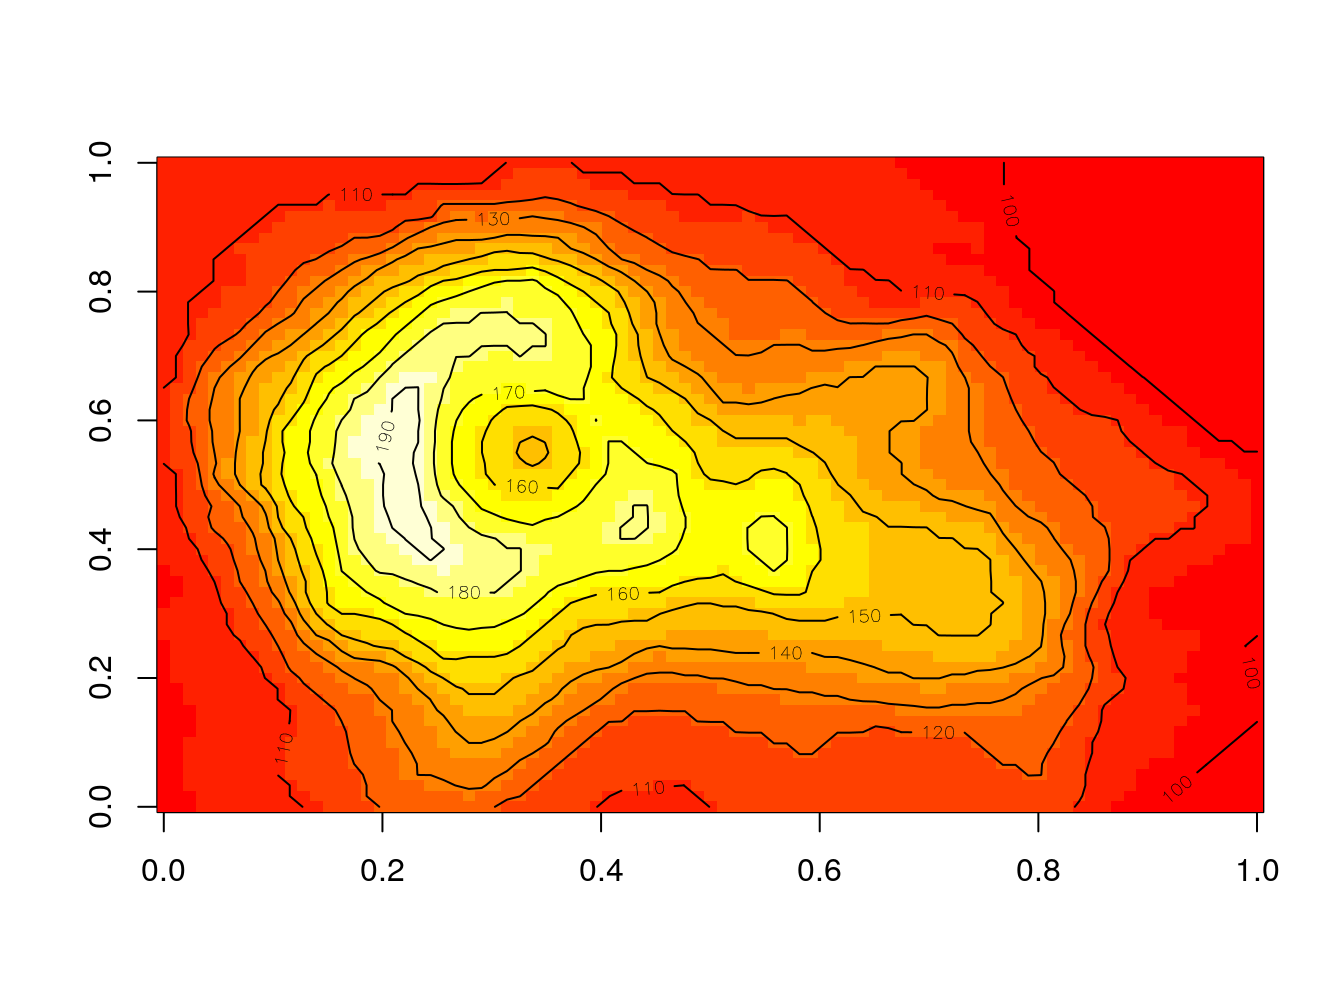
\includegraphics[width=0.8\linewidth]{ksiazka_files/figure-latex/nice-fig-1} 

}

\caption{Wulkan - rzut z góry}\label{fig:nice-fig}
\end{figure}

\begin{figure}

{\centering 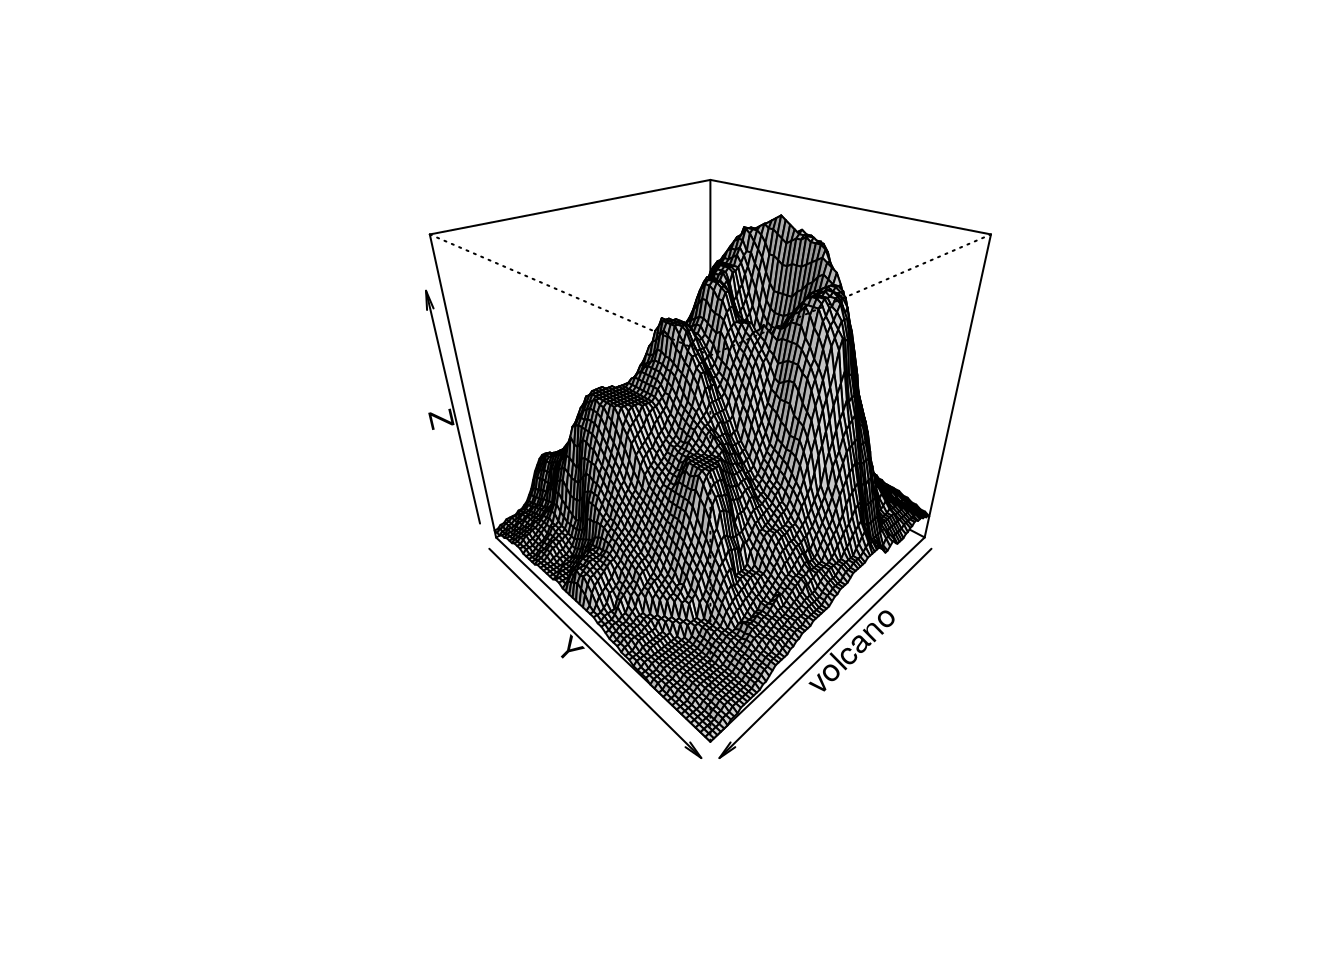
\includegraphics{ksiazka_files/figure-latex/nice-fig2-1} 

}

\caption{Wulkan - rzut perspektywiczny}\label{fig:nice-fig2}
\end{figure}

\subsection*{Zadanie domowe}\label{zadanie-domowe-1}
\addcontentsline{toc}{subsection}{Zadanie domowe}

\begin{enumerate}
\def\labelenumi{\arabic{enumi}.}
\tightlist
\item
  Wykonaj przykłady z podręcznika P. Biecka dotyczące ramek danych i
  macierzy
\item
  Przeczytaj z ww. podręcznika rozdział dotyczący list i ogólnego
  schematu pracy na danych tego typu
\end{enumerate}

\subsection*{Zadania sprawdzające}\label{zadania-sprawdzajace-2}
\addcontentsline{toc}{subsection}{Zadania sprawdzające}

\url{https://goo.gl/forms/QkiVqWIiDJlrhLAQ2}

\chapter{Wczyt i zapis danych}\label{wczyt-i-zapis-danych}

Elementarną umiejętnością pracy na danych w \textbf{R} jest możliwość
zaczytania wybranego/dowolnego formatu oraz dalsza praca już na danych
dostępnych w środowisku \textbf{R}/\textbf{RStudio}. Prawdopodobnie
dotychczas dane zapisywałeś(aś) w formatach arkuszy kalkulacyjnych
(xls/xlsx/ods). Tymczasem w naukach atmosferycznych jest to w
rzeczywistości jeden z najrzadziej wykorzystywanych formatów\ldots{}

\textbf{R} obsługuje bardzo szeroką gamę formatów danych, a te które nie
są natywnie wspierane zwykle mogą być zaimportowane do \textbf{R} za
pomocą bezpłatnych bibliotek. W ten sposób w \textbf{R} można
jednocześnie pracować w jednym środowisku na różnych danych, bez
konieczności \emph{przełączania} się za każdym razem do programu
obsługującego dany format lub posiadającego dane możliwości (np.
pobranie danych -\textgreater{} przygotowanie danych przestrzennych
-\textgreater{} wizualizacja w postaci mapy).

W naukach atmosferycznych najczęściej stosowane formaty danych
obsługiwane przez \textbf{R} to:

\begin{itemize}
\tightlist
\item
  Dane przechowywane w formie ``tabelarycznej'' (np.: \texttt{csv},
  \texttt{ASCII}, \texttt{xls/xlsx}, \texttt{GoogleSheets} oraz w
  postaci bazodanowej (np. \texttt{SQL} i pochodne)).
\item
  Formaty danych specjalistycznych GIS: (np.
  \texttt{HDF4,\ HDF5,\ GeoTIFF,\ Shapefile,\ ASC} i innych wspieranych
  przez bibliotekę \texttt{GDAL}).
\item
  Specjalistyczne formaty danych meteorologicznych (np.
  \texttt{GRIB,\ NetCDF-3,\ NetCDF-4}).
\end{itemize}

\section{Katalog roboczy}\label{katalog-roboczy}

Zanim przejdziemy do wczytywania danych musimy zaznajomić się ze
sposobem ustalania katalogów roboczych \textbf{R}. Domyślnie po
uruchomieniu \textbf{R} pracujemy w katalogu domowym, który może być
zlokalizowany w różnych miejscach dysku. Aby sprawdzić obecny katalog
roboczy (ang. \emph{Workind directory}) należy posłużyć się funkcję
\texttt{getwd()} bez żadnych dodatkowych argumentów

\begin{Shaded}
\begin{Highlighting}[]
\KeywordTok{getwd}\NormalTok{()}
\end{Highlighting}
\end{Shaded}

\begin{verbatim}
## [1] "/home/bartosz/github/przetwarzanie"
\end{verbatim}

Jeśli chcemy zmienić katalog roboczy możemy to zrobić na 3 różne
sposoby:

\begin{enumerate}
\def\labelenumi{\arabic{enumi}.}
\item
  Użyć funkcji \texttt{setwd()} podając ścieżkę do wybranego katalogu
  (wersja zaawansowana)
\item
  Wybrać z górnego menu \textbf{RStudio} opcję \texttt{Session},
  następnie \texttt{Set\ working\ directory} i następnie
  \texttt{Choose\ directory}, analogicznie do zrzutu na poniższym
  ekranie. Ważne aby ustawić jedynie KATALOG a nie PLIK w którym
  będziemy pracować i przechowywać nasze dane. Po poprawnym wskazaniu
  katalogu roboczego w konsoli pojawi się wynik działania jako wywołana
  funkcja \texttt{setwd()} ze wskazanym katalogiem.
\item
  Analogiczny efekt jak w pkt. 2 można uzyskać za pomocą skrótu
  klawiszowego \texttt{ctrl+shift+h}
\end{enumerate}

\begin{figure}
\centering
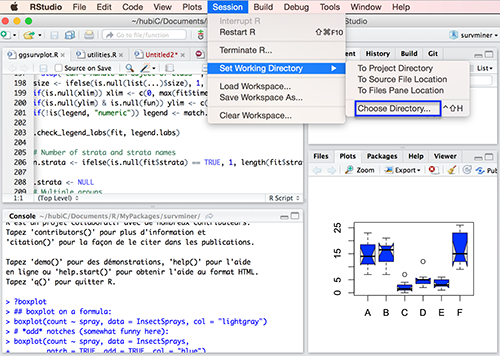
\includegraphics{figures/rstudio_setwd.png}
\caption{Wybór katalogu roboczego w \textbf{RStudio}}
\end{figure}

W tym momencie wszystkie pliki znajdujące się naszym katalogu mogą być
od razu znalezione przez \textbf{R} (tj. bez wpisywania pełnej ścieżki
do pliku). Jeśli chcesz sprawdzić jakie to są pliki zawsze możesz użyć
funkcji \texttt{dir()} wyświetlającej zawartość obecnego katalogu
roboczego \texttt{dir()}.

\section{Wczyt danych}\label{wczyt-danych}

Dane do ćwiczeń pobierz ze strony:
\url{http://www.enwo.pl/przetwarzanie/dane} i zapisz je na Pulpicie w
folderze \texttt{dane} lub w innej znanej lokalizacji. Następnie ustaw
katalog roboczy na odpowiedni folder z pobranymi plikami. Z poziomu
konsoli \textbf{R} sprawdź zawartość katalogu poleceniem \texttt{dir()}.
W wyniku powinieneś otrzymać następujące pliki:

\subsection{Format tekstowy (CSV i
pokrewne)}\label{format-tekstowy-csv-i-pokrewne}

Naukę wczytywania danych rozpoczniemy od danych tabelarycznych
zapisanych w formacie tekstowym. Pomimo wielu technicznych aspektów
powodujących problemy, jest to w dalszym ciągu najbardziej uniwersalny
format wymiany i zapisu danych. Najczęściej pliki przechowujące dane w
takim kształcie mają rozszerzenie \texttt{.csv} od wyrażenia \emph{comma
separeted value} (ang. \emph{wartości rozdzielone przecinkami}),
\texttt{.tsv} (wartości rozdzielone znakami tabulacji), \texttt{.asc}
lub po prostu \texttt{.txt}. Należy przy tym zaznaczyć, że rozszerzenie
pliku nie jest przez \textbf{R} brane pod uwagę i dlatego użytkownik
musi precyzyjnie zadeklarować wszystkie ustawienia związane z wczytem
danych!

Do wczytywania danych teksowych najczęściej stosowana jest funkcja:
\texttt{read.table()} lub w nieco zmodyfikowanej wersji funkcja
\texttt{read.csv()}. Obie funkcje są bardzo podobne jeśli chodzi o
sposób użycia i różnią się na ogół domyślnymi wartościami argumentów.
Przed próbą wczytania pliku tektsowego do \textbf{R} należy w pierwszej
kolejności zapoznać się z jego strukturą. W tym celu otwórz plik
\texttt{pl1.csv} za pomocą notatnika lub innego edytora tekstowego i
zapisz na kartce:

\begin{itemize}
\tightlist
\item
  czy plik ma nazwy kolumn/wierszy?
\item
  czy dane w poszczególnych kolumnach (poza nazwami kolumny/wierszy) są
  tylko typu liczbowego?
\item
  jaki znak jest separatorem miejsc dziesiętnych?
\item
  jaki znak rozdziela kolejne pola?
\item
  czy braki danych są zapisane w inny sposób niż poprzez wartości NA
  (częstym standardem jest stosowanie np. zapisu -9999, -99.99, ---,
  pozostawianie pustego pola, itp.)?
\end{itemize}

Te informacje są niezbędne do ustawienia poszczególnych argumentów
funkcji \texttt{read.table()} lub \texttt{read.csv()}. Najważniejsze z
nich:

\begin{itemize}
\tightlist
\item
  \texttt{file} - pełna ścieżka do pliku lub po prostu nazwa pliku
  (jeśli znajduje się w katalogu roboczym), możliwe jest także podanie
  adresu internetowego
\item
  \texttt{header} - czy plik posiada nagłówek (podpisane nazwy kolumn) w
  pierwszym wierszu? Domyślnie wartość tego parametru jest ustawiona na
  \texttt{TRUE}
\item
  \texttt{sep} - seperator kolumn - jaki znak rozdziela wartości w
  poszczególnych kolumnach. Może być to średnik (``;''), przecinek
  (``,''), spacja (" ``), tabulator (\texttt{\textbackslash{}t}), lub
  inny dowolnie zadeklarowany znak w cudzysłowiu
\item
  \texttt{dec} - separator miejsc dziesiętnych. Analogicznie jak dla
  opcji separatora kolumn
\item
  \texttt{na.strings} - sposób zapisu i traktowania braków danych
\item
  \texttt{stringsAsFactors} - czy wartości tekstowe mają być traktowane
  jako typ czynnikowy (domyślnie \texttt{TRUE}, ale zwykle warto zmienić
  na \texttt{FALSE})
\item
  \ldots{} reszta opcji dostępna we wbudowanej pomocy funkcji
  \texttt{read.table()} )
\end{itemize}

Znając powyższe argumenty i po zaznajomieniu się z wbudowaną pomocą
spróbuj użyć funkcji\\
\texttt{read.csv()} do wczytu przeglądanego pliku. Plik ma rozszerzenie
.csv i jest rozdzielony spacjami, więc intuicyjnie rzecz biorąc powinna
być to najlepsza opcja. W razie konieczności otwórz okno pomocy dla
testowanej funkcji.

\begin{Shaded}
\begin{Highlighting}[]
\KeywordTok{read.csv}\NormalTok{(}\StringTok{"pl1.csv"}\NormalTok{)}
\end{Highlighting}
\end{Shaded}

\begin{verbatim}
##     rok      I    II   III    IV     V    VI   VII  VIII    IX     X    XI
## 1  1971  -2.96  0.37 -0.11  7.41 14.48 14.91 17.81 18.74 11.25  8.39  2.61
## 2  1972  -5.81  0.27  3.91  7.36 12.48 16.25 19.40 16.56 11.36  6.14  4.36
## 3  1973  -1.67  1.27  3.69  6.13 12.35 15.77 17.58 17.12 13.14  6.62  1.85
## 4  1974   0.06  2.29  4.37  6.89 10.75 14.04 15.62 17.70 13.40  6.29  3.86
## 5  1975   2.97 -0.56  3.87  6.58 13.35 15.40 18.55 18.27 15.79  7.98  1.75
## 6  1976  -1.97 -3.32 -0.85  6.72 11.95 15.09 18.06 15.31 12.58  7.59  4.71
## 7  1977  -1.43  0.46  5.04  5.74 12.02 16.60 15.97 15.98 11.08  9.17  5.03
## 8  1978  -0.95 -3.08  3.53  5.88 11.40 14.93 15.75 15.66 11.32  8.78  4.60
## 9  1979  -5.46 -4.58  2.30  6.23 13.81 18.23 14.73 16.50 13.31  6.50  2.94
## 10 1980  -5.90 -1.14 -0.01  5.66  9.29 15.03 16.12 16.02 12.65  8.36  2.03
## 11 1981  -2.98 -0.97  4.50  5.88 13.78 16.47 17.20 16.36 13.76  8.61  3.43
## 12 1982  -4.12 -2.11  3.69  5.43 13.05 15.62 18.33 18.40 15.23  9.27  4.96
## 13 1983   3.15 -2.37  4.04  9.25 14.38 16.15 19.00 17.86 14.12  8.87  2.45
## 14 1984   0.08 -1.52  1.02  7.75 12.84 14.03 15.52 17.47 12.80 10.46  2.83
## 15 1985  -8.14 -7.56  2.05  7.41 14.07 13.96 17.04 17.26 12.36  8.39  0.57
## 16 1986  -1.33 -8.79  1.96  7.80 14.38 15.68 17.30 16.75 11.09  8.50  5.15
## 17 1987 -10.68 -1.46 -2.46  7.04 10.84 15.16 17.37 15.11 13.23  8.83  4.28
## 18 1988   1.39  1.09  1.09  7.02 14.14 15.80 18.52 17.06 13.50  8.23  0.34
## 19 1989   1.75  3.56  5.51  8.74 13.18 15.10 17.85 17.32 14.37 10.24  2.03
## 20 1990   1.80  4.92  6.50  7.92 13.29 16.13 16.62 17.48 11.30  9.21  4.60
## 21 1991   0.18 -3.91  4.44  7.23  9.72 14.69 18.68 17.77 14.24  7.95  3.82
## 22 1992  -0.54  1.50  3.56  7.41 13.10 17.78 19.34 20.59 12.94  6.01  3.86
## 23 1993   0.35 -1.05  1.48  8.62 15.61 15.08 16.31 16.26 12.11  8.28 -1.27
## 24 1994   2.24 -2.41  4.11  8.58 12.05 16.08 20.96 18.18 14.43  6.80  4.21
## 25 1995  -1.20  3.33  2.78  7.62 12.09 16.04 19.78 18.04 12.98 10.45  0.63
## 26 1996  -5.31 -5.08 -1.35  7.62 13.28 16.09 15.89 17.82 10.36  9.24  5.56
## 27 1997  -4.34  2.00  3.13  4.98 12.83 16.41 17.45 18.91 13.29  6.74  3.00
## 28 1998   1.12  3.56  2.14  9.69 13.80 17.02 17.23 16.32 13.29  7.96 -0.78
## 29 1999   0.47 -0.96  4.51  9.17 12.49 16.75 19.68 17.32 15.99  8.52  2.39
## 30 2000  -1.01  2.54  3.62 11.50 14.63 16.88 16.12 17.79 12.16 11.77  6.64
##      XII
## 1   3.02
## 2  -0.01
## 3  -0.72
## 4   2.73
## 5   0.88
## 6  -1.24
## 7  -0.38
## 8  -3.03
## 9   2.14
## 10 -0.12
## 11 -3.20
## 12  1.22
## 13 -0.64
## 14 -1.09
## 15  2.16
## 16  0.02
## 17  0.76
## 18  1.10
## 19  1.16
## 20 -0.18
## 21 -0.93
## 22 -0.54
## 23  1.97
## 24  1.38
## 25 -4.44
## 26 -4.88
## 27  0.41
## 28 -1.69
## 29  0.91
## 30  1.92
\end{verbatim}

Wygląda na to, że wszystko wczytało się poprawnie. Samo wyświetlenie
zawartości pliku nie pozwala na dalszą pracę z danymi w \textbf{R}.
Musimy wynik polecenia wczytać do zmiennej (za pomocą
\texttt{\textless{}-} , \texttt{=} lub \texttt{-\textgreater{}}) aby był
widoczny zakładce `Environment' pod wskazaną nazwą. Nazwijmy ten obiekt
`dane' i przejrzyjmy jego zawartość za pomocą graficznej przeglądarki
ramek danych lub fragmentarycznie w konsoli.

\begin{Shaded}
\begin{Highlighting}[]
\NormalTok{dane <-}\StringTok{ }\KeywordTok{read.csv}\NormalTok{(}\StringTok{"pl1.csv"}\NormalTok{)}
\KeywordTok{head}\NormalTok{(dane)}
\end{Highlighting}
\end{Shaded}

\begin{verbatim}
##    rok     I    II   III   IV     V    VI   VII  VIII    IX    X   XI
## 1 1971 -2.96  0.37 -0.11 7.41 14.48 14.91 17.81 18.74 11.25 8.39 2.61
## 2 1972 -5.81  0.27  3.91 7.36 12.48 16.25 19.40 16.56 11.36 6.14 4.36
## 3 1973 -1.67  1.27  3.69 6.13 12.35 15.77 17.58 17.12 13.14 6.62 1.85
## 4 1974  0.06  2.29  4.37 6.89 10.75 14.04 15.62 17.70 13.40 6.29 3.86
## 5 1975  2.97 -0.56  3.87 6.58 13.35 15.40 18.55 18.27 15.79 7.98 1.75
## 6 1976 -1.97 -3.32 -0.85 6.72 11.95 15.09 18.06 15.31 12.58 7.59 4.71
##     XII
## 1  3.02
## 2 -0.01
## 3 -0.72
## 4  2.73
## 5  0.88
## 6 -1.24
\end{verbatim}

\subsubsection*{Usunięcie zmiennej}\label{usuniecie-zmiennej}
\addcontentsline{toc}{subsubsection}{Usunięcie zmiennej}

Każdy obiekt zaczytany do pamięci operacyjnej widoczny w prawym górnym
rogu w zakładce \texttt{Environment} zmniejsza dostępną pamięć dla
następnych obiektów. Jeśli chcemy się pozbyć wszystkich zadeklarowanych
obiektów możemy kliknąć w symbol pędzelka w prawym górnym rogu i
potwierdzić chęć usunięcia wszystkich obiektów.

W przypadku gdy chcemy usunąć tylko wskazane obiekty możemy posłużyć się
funkcją \texttt{rm()} wpisując jako argument nazwę obiektu (bez
cudzysłowia), którego chcemy się pozbyć. Jeśli pracujemy w środowisku
\textbf{R} (a nie \textbf{RStudio}) to nazwy bieżących zmiennych możemy
wyświetlić za pomocą funkcji \texttt{ls()}.

\subsection*{Zadania kontrolne}\label{zadania-kontrolne}
\addcontentsline{toc}{subsection}{Zadania kontrolne}

\begin{enumerate}
\def\labelenumi{\arabic{enumi}.}
\tightlist
\item
  Na podstawie wczytanego zbioru danych oblicz średnią roczną
  temperaturę powietrza w roku 1971 i 2000
\item
  Oblicz średnią temperaturę stycznia i grudnia w wieloleciu 1971-2000
\item
  Sprawdź w sytemie pomocy działanie funkcji \texttt{boxplot()}.
  Następnie zastosuj ją do wczytanego zbioru danych. 3.1. Wywołaj
  jeszcze raz funkcję \texttt{boxplot()} ale bez wartości dla pierwszej
  kolumny (dla lat)
\item
  Wczytaj pozostałe zbiory danych tekstowych (tj. \texttt{pl2.tsv},
  \texttt{pl3.csv}, \texttt{pl4.txt}) korzystając z funkcji
  \texttt{read.csv()} lub \texttt{read.table()}
\end{enumerate}

\subsubsection{Wczyt danych bezpośrednio z
internetu}\label{wczyt-danych-bezposrednio-z-internetu}

W odróżnieniu od pracy w arkuszach kalkulacyjnych \textbf{R} w wielu
przypadkach nie wymaga wcześniejszego zapisu danych na dysku! Dane można
wczytać bezpośrednio np. z internetu:

\begin{Shaded}
\begin{Highlighting}[]
\KeywordTok{read.table}\NormalTok{(}\StringTok{"http://biecek.pl/MOOC/dane/koty_ptaki.csv"}\NormalTok{, }\DataTypeTok{sep=}\StringTok{";"}\NormalTok{, }\DataTypeTok{dec=}\StringTok{","}\NormalTok{, }\DataTypeTok{header=}\OtherTok{TRUE}\NormalTok{)}
\end{Highlighting}
\end{Shaded}

\begin{verbatim}
##           gatunek   waga dlugosc predkosc  habitat zywotnosc druzyna
## 1          Tygrys 300.00     2.5       60     Azja        25     Kot
## 2             Lew 200.00     2.0       80   Afryka        29     Kot
## 3          Jaguar 100.00     1.7       90  Ameryka        15     Kot
## 4            Puma  80.00     1.7       70  Ameryka        13     Kot
## 5         Leopard  70.00     1.4       85     Azja        21     Kot
## 6          Gepard  60.00     1.4      115   Afryka        12     Kot
## 7           Irbis  50.00     1.3       65     Azja        18     Kot
## 8          Jerzyk   0.05     0.2      170 Euroazja        20    Ptak
## 9           Strus 150.00     2.5       70   Afryka        45    Ptak
## 10  Orzel przedni   5.00     0.9      160   Polnoc        20    Ptak
## 11 Sokol wedrowny   0.70     0.5      110   Polnoc        15    Ptak
## 12 Sokol norweski   2.00     0.7      100   Polnoc        20    Ptak
## 13       Albatros   4.00     0.8      120 Poludnie        50    Ptak
\end{verbatim}

\subsection{Pliki tekstowe o stałej szerokości
kolumn}\label{pliki-tekstowe-o-staej-szerokosci-kolumn}

Zdarza się, że dane są zapisywane w formacie plików o odgórnie ustalonej
szerokości plików (tzw. Fixed Width Format Files). Przykładowe dane w
takim formacie umieszczono pod adresem
\url{http://enwo.pl/przetwarzanie/dane/poz.txt}

Wczyt takiego formatu w \textbf{R} umożliwia funkcja
\texttt{read.fwf()}, która oprócz wskazania nazwy pliku wymaga
deklaracji argumentu \texttt{widths} w formie wektora oznaczającego
szerokość poszczególnych kolumn. Przed wczytaniem pliku należy zatem
dokładnie policzyć ile znaków (szerokości) zajmują pola poszczególnych
kolumn. Wspomniany przed momentem plik z danymi meteorologicznymi dla
Poznania zapiszmy na dysku. Powinien zawierać:

\begin{itemize}
\tightlist
\item
  5 znaków dla kodu stacji
\item
  30 znaków dla nazwy stacji
\item
  4 znaki dla roku
\item
  2 znaki dla miesięcy
\item
  2 znaki dla dni
\item
  8 znaków dla dobowych sum opadów atmosferycznych. \emph{Brak opadu
  zapisany jest jako .09 w 3 ostatnich znakach pola}
\item
  7 znaków dla dobowej temperatury powietrza
\end{itemize}

Zatem pełna komenda wczytująca wspomniany plik oraz 2 komendy
wyświetlające szybkie podsumowanie mogą wyglądać następująco:

\begin{Shaded}
\begin{Highlighting}[]
\NormalTok{dane <-}\StringTok{ }\KeywordTok{read.fwf}\NormalTok{(}\StringTok{"poz.txt"}\NormalTok{,}\DataTypeTok{widths =} \KeywordTok{c}\NormalTok{(}\DecValTok{5}\NormalTok{,}\DecValTok{30}\NormalTok{,}\DecValTok{4}\NormalTok{,}\DecValTok{2}\NormalTok{,}\DecValTok{2}\NormalTok{,}\DecValTok{8}\NormalTok{,}\DecValTok{7}\NormalTok{), }\DataTypeTok{na.strings=}\StringTok{"     .09"}\NormalTok{)}
\KeywordTok{summary}\NormalTok{(dane) }\CommentTok{# wyswietlenie}
\end{Highlighting}
\end{Shaded}

\begin{verbatim}
##        V1                                   V2              V3      
##  Min.   :330   poznan                        :17167   Min.   :1966  
##  1st Qu.:330                                          1st Qu.:1977  
##  Median :330                                          Median :1989  
##  Mean   :330                                          Mean   :1989  
##  3rd Qu.:330                                          3rd Qu.:2001  
##  Max.   :330                                          Max.   :2012  
##                                                                     
##        V4               V5              V6               V7       
##  Min.   : 1.000   Min.   : 1.00   Min.   : 0.000   Min.   :-21.9  
##  1st Qu.: 4.000   1st Qu.: 8.00   1st Qu.: 0.000   1st Qu.:  2.5  
##  Median : 7.000   Median :16.00   Median : 0.700   Median :  8.8  
##  Mean   : 6.523   Mean   :15.73   Mean   : 2.419   Mean   :  8.7  
##  3rd Qu.:10.000   3rd Qu.:23.00   3rd Qu.: 2.900   3rd Qu.: 15.3  
##  Max.   :12.000   Max.   :31.00   Max.   :85.700   Max.   : 29.7  
##                                   NA's   :6973
\end{verbatim}

\begin{Shaded}
\begin{Highlighting}[]
\KeywordTok{hist}\NormalTok{(dane}\OperatorTok{$}\NormalTok{V6[dane}\OperatorTok{$}\NormalTok{V6}\OperatorTok{>}\DecValTok{30}\NormalTok{]) }\CommentTok{# histogram częstości występowania opadów > 30mm/dobę}
\end{Highlighting}
\end{Shaded}

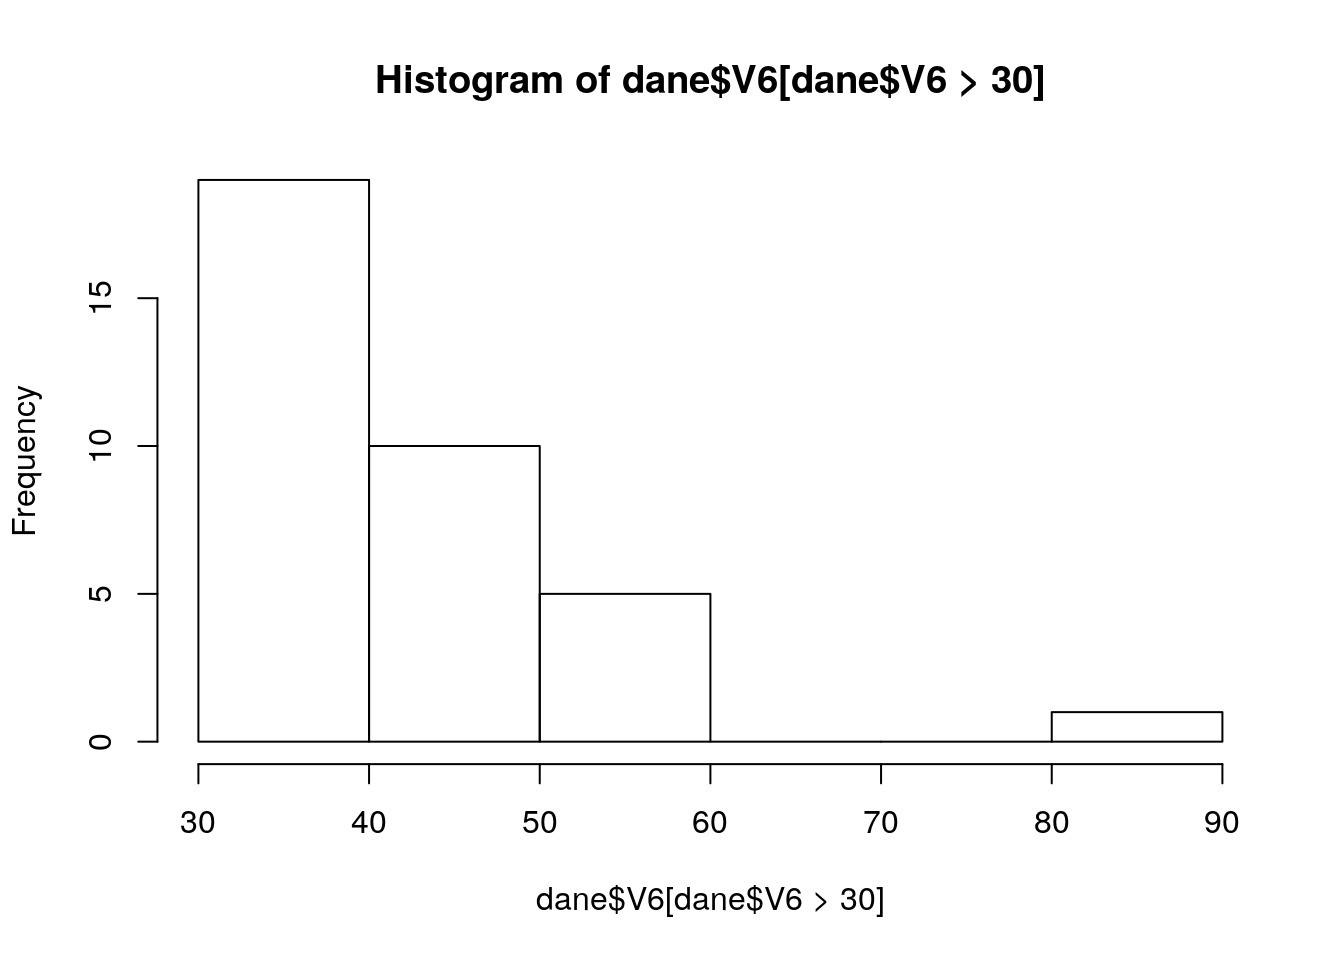
\includegraphics{ksiazka_files/figure-latex/readfwf1-1.pdf}

\subsection{Format Excela (.xls /
.xlsx)}\label{format-excela-.xls-.xlsx}

Dane pochodzące z arkuszów kalkulacyjnych zwykle są zapisywane w postaci
plików \texttt{.xls} lub \texttt{.xlsx}. Nie jest to najbardziej
``szczęśliwy'' format do pracy w \textbf{R} ze względu na brak
jednoznacznej interpretacji niektórych zapisów i formatowania (np. dat).

Jeśli mamy dane we wspomnianych formatach najczęściej stosuje się 2
rozwiązania:

\begin{enumerate}
\def\labelenumi{\arabic{enumi}.}
\tightlist
\item
  Eksport danych z arkusza kalkulacyjnego do formatu tekstowego (np.
  \texttt{csv})
\item
  Wykorzystanie bezpłatnych pakietów np.
  \texttt{readxl,\ XLconnect,\ openxlsx,\ gdata,\ xlsReadWrite,\ xlsx}\ldots{}
\end{enumerate}

Spróbujmy zastosować oba rozwiązania do plików \texttt{pl5.xls} oraz
\texttt{pl6.xlsx} \ldots{}

\subsection{\texorpdfstring{Format binarny
\textbf{R}}{Format binarny R}}\label{format-binarny-r}

Najbardziej efektywnym sposobem przechowywania danych w \textbf{R} jest
format binarny, który pozwala na szybki zapis i odczyt danych. Dane w
tym formacie mają najczęściej rozszerzenie \texttt{.rda} lub
\texttt{.Rdata} i mogą być wczytane za pomocą funkcji \texttt{load()},
przy czym w pliku może się znajdować więcej niż 1 obiekt, stąd też
zmienne bezpośrednio są ładowane do środowiska bez możliwości
deklarowania ich nazwy.

Spróbujmy pobrać przykładowe dane z adresu
\url{http://www.enwo.pl/przetwarzanie/dane/pm10.Rdata} i zapiszmy je na
dysku. Następnie wczytajmy je za pomocą funkcji \texttt{load()} i
przejrzyjmy ich zawartość.

\begin{Shaded}
\begin{Highlighting}[]
\KeywordTok{load}\NormalTok{(}\StringTok{"dane/pm10.Rdata"}\NormalTok{)}
\KeywordTok{head}\NormalTok{(ogrody_d)}
\end{Highlighting}
\end{Shaded}

\begin{verbatim}
##         date   yy mm dd   hh       ws       wd     pm10     air_t      slp
## 1 2005-01-01 2005  1  1 12.0 3.826087 275.5945 25.61364 0.2545455 1013.182
## 2 2005-01-02 2005  1  2 11.5 7.583333 253.0708 19.56250 0.3083333 1004.083
## 3 2005-01-03 2005  1  3 11.5 7.833333 267.5562 10.91667 0.1541667 1009.417
## 4 2005-01-04 2005  1  4 11.5 9.041667 271.8748 12.73913 0.4608696 1008.174
## 5 2005-01-05 2005  1  5 11.5 6.291667 260.1847 19.00000 2.1250000 1013.083
## 6 2005-01-06 2005  1  6 11.5 5.750000 259.3237 21.23913 2.8043478 1013.826
\end{verbatim}

\begin{Shaded}
\begin{Highlighting}[]
\KeywordTok{head}\NormalTok{(polanka_d)}
\end{Highlighting}
\end{Shaded}

\begin{verbatim}
##         date   yy mm dd   hh       ws       wd      pm10 pm25
## 1 2005-01-01 2005  1  1 12.0 3.826087 275.5945 21.543478   NA
## 2 2005-01-02 2005  1  2 11.5 7.583333 253.0708 12.291667   NA
## 3 2005-01-03 2005  1  3 11.5 7.833333 267.5562  9.666667   NA
## 4 2005-01-04 2005  1  4 11.5 9.041667 271.8748  8.395833   NA
## 5 2005-01-05 2005  1  5 11.5 6.291667 260.1847 18.978261   NA
## 6 2005-01-06 2005  1  6 11.5 5.750000 259.3237 19.875000   NA
\end{verbatim}

Jeśli chcemy zaczytać plik bezpośrednio z internetu musimy funkcję
\texttt{load()} o tym poinformować korzystając dodatkowo z funkcji
\texttt{url()}:

\begin{Shaded}
\begin{Highlighting}[]
\KeywordTok{load}\NormalTok{(}\KeywordTok{url}\NormalTok{(}\StringTok{"http://biecek.pl/MOOC/dane/koty_ptaki.rda"}\NormalTok{))}
\NormalTok{koty_ptaki}
\end{Highlighting}
\end{Shaded}

\begin{verbatim}
##           gatunek   waga dlugosc predkosc  habitat zywotnosc druzyna
## 1          Tygrys 300.00     2.5       60     Azja        25     Kot
## 2             Lew 200.00     2.0       80   Afryka        29     Kot
## 3          Jaguar 100.00     1.7       90  Ameryka        15     Kot
## 4            Puma  80.00     1.7       70  Ameryka        13     Kot
## 5         Leopard  70.00     1.4       85     Azja        21     Kot
## 6          Gepard  60.00     1.4      115   Afryka        12     Kot
## 7           Irbis  50.00     1.3       65     Azja        18     Kot
## 8          Jerzyk   0.05     0.2      170 Euroazja        20    Ptak
## 9           Strus 150.00     2.5       70   Afryka        45    Ptak
## 10  Orzel przedni   5.00     0.9      160   Polnoc        20    Ptak
## 11 Sokol wedrowny   0.70     0.5      110   Polnoc        15    Ptak
## 12 Sokol norweski   2.00     0.7      100   Polnoc        20    Ptak
## 13       Albatros   4.00     0.8      120 Poludnie        50    Ptak
\end{verbatim}

\subsection{RDS}\label{rds}

Jeśli chcemy pozostawić dowolność co do nazwy wczytywanego obiektu
częstą alternatywą jest format \texttt{.rds}, który również jest
wewnętrznym formatem środowiska \textbf{R}, ale przechowuje jeden
obiekt, stąd też zwykle wczytuje się go do zmiennej. Funkcja do odczytu
tego formatu to \texttt{readRDS()}. Warto zaznaczyć, że ta funkcja
działa intuicyjnie jedynie w odniesieniu do lokalnych plików.

Zapiszmy na dysku przykładowy plik znajdujący się pod adresem:
\href{http://www.enwo.pl/przetwarzanie/dane/pm10_new.rds}{http://www.enwo.pl/przetwarzanie/datne/pm10\_new.rds},
a następnie wczytajmy go do obiektu \texttt{poznan}

\begin{Shaded}
\begin{Highlighting}[]
\NormalTok{poznan <-}\StringTok{ }\KeywordTok{readRDS}\NormalTok{(}\StringTok{"dane/pm10_new.rds"}\NormalTok{)}
\KeywordTok{head}\NormalTok{(poznan,}\DecValTok{4}\NormalTok{) }\CommentTok{# pokazuje tylko 4 pierwsze linie ramki danych}
\end{Highlighting}
\end{Shaded}

\begin{verbatim}
##         data   yy mm dd tmax tmin tavg tdavg rhavg  wd   ws gust    slp
## 1 2005-01-01 2005  1  1  5.9  3.6  4.9   4.3  95.7 WSW 16.8   NA 1019.3
## 2 2005-01-02 2005  1  2  6.1  0.1  3.6   1.8  89.7 WSW 13.3   NA 1016.7
## 3 2005-01-03 2005  1  3  6.8  1.1  4.1  -0.2  74.4   W 32.0 68.4 1011.2
## 4 2005-01-04 2005  1  4  6.2  2.0  3.8   1.5  84.7   W 28.4   NA 1015.8
##   prec totcl lowcl sun  vis snow ogrodypm10 polankapm10 polankapm25
## 1  3.5   8.0   8.0 0.0  4.6    0   25.61364   21.543478          NA
## 2  0.4   7.0   7.0 0.0  9.8    0   19.56250   12.291667          NA
## 3  0.6   5.5   5.5 1.8 15.9    0   10.91667    9.666667          NA
## 4  4.7   7.2   7.2 1.2 13.8    0   12.73913    8.395833          NA
##   poznanpm10 maxwind wd_deg ws_avg    u     v przekroczenie50poz pm10_m1
## 1      25.61    16.8 275.59   3.83 3.81 -0.37                  0   16.43
## 2      19.56    13.3 253.07   7.58 7.25  2.21                  0   25.61
## 3      10.92    68.4 267.56   7.83 7.82  0.33                  0   19.56
## 4      12.74    28.4 271.87   9.04 9.04 -0.29                  0   10.92
##   pm10_m2 pm10_m3 pm10_m4 pm10_m5 pm10_m6 pm10_m7
## 1   10.60    7.56   11.16   19.44   17.35   12.38
## 2   16.43   10.60    7.56   11.16   19.44   17.35
## 3   25.61   16.43   10.60    7.56   11.16   19.44
## 4   19.56   25.61   16.43   10.60    7.56   11.16
\end{verbatim}

\begin{enumerate}
\def\labelenumi{\arabic{enumi}.}
\tightlist
\item
  Narysuj histogram koncentracji dobowej PM10 w Poznaniu.
\item
  Oblicz wartości statystyk testowych dla wczytanego zbioru danych.
\end{enumerate}

\section{Zapis danych}\label{zapis-danych}

Wspomniane powyżej instrukcje wczytywania danych mają najczęściej swoje
odpowiedniki dla zapisu poprzez zamianę słowa kluczowego funkcji
\texttt{read} lub \texttt{load} na \texttt{write} lub \texttt{save}.
Jako że zapis danych zwykle jest łatwiejszy niż wczyt zagadnienie to
zostanie omówione w dużym skróciew kolejnych częściach niniejszego
rozdziału. W przypadkach wątpliwych zawsze warto korzystać z wbudowanego
systemu pomocy lub z podręcznika P. Biecka \citep{biecek2016}.

\subsection{Dane tekstowe (csv i
pokrewne)}\label{dane-tekstowe-csv-i-pokrewne}

Zapis zmiennej będącej wektorem, macierzą lub ramką danych do postaci
tekstowej możliwy jest za pomocą funkcji \texttt{write.table()} lub
\texttt{write.csv()} / \texttt{write.csv2()}. Argumenty funkcji
dopasowujące format zapisu i ich wartości domyślne można sprawdzić za
pomocą polecenia \texttt{?write.table}. W zdecydowanej większości są one
analogiczne lub bardzo podobne do argumentów funkcji wczytujących.

\textbf{Zadanie kontrolne:}

\begin{enumerate}
\def\labelenumi{\arabic{enumi}.}
\tightlist
\item
  Wczytaj do \textbf{R} zbiór danych ze średnimi temperaturami powietrza
  w Polsce w latach 1971-2000 (np. z pliku \texttt{pl1.csv}) i nazwij go
  \texttt{dane}
\item
  Zaokrągl wartości temperatur powietrza do 1 miejsca po przecinku i
  zapisz je jako obiekt \texttt{dane2}
\item
  Wyświetl pierwsze kilka wierszy nowej ramki danych funkcją
  \texttt{head()} w celu upewnienia się co do poprawności poprzedniej
  operacji
\item
  Zapisz obiekt \texttt{dane2} do pliku \texttt{dane2.txt}. Kolumny
  rozdziel znakiem \texttt{;}, miejsca dziesiętne przecinkiem. W pliku
  będą zawarte nazwy kolumn, bez nazwy wierszy.
\end{enumerate}

Przykładowe rozwiązanie:

\begin{Shaded}
\begin{Highlighting}[]
\NormalTok{dane <-}\StringTok{ }\KeywordTok{read.csv}\NormalTok{(}\StringTok{"pl1.csv"}\NormalTok{)}
\NormalTok{dane2 <-}\StringTok{ }\KeywordTok{round}\NormalTok{(dane, }\DecValTok{1}\NormalTok{)}
\KeywordTok{head}\NormalTok{(dane2)}
\end{Highlighting}
\end{Shaded}

\begin{verbatim}
##    rok    I   II  III  IV    V   VI  VII VIII   IX   X  XI  XII
## 1 1971 -3.0  0.4 -0.1 7.4 14.5 14.9 17.8 18.7 11.2 8.4 2.6  3.0
## 2 1972 -5.8  0.3  3.9 7.4 12.5 16.2 19.4 16.6 11.4 6.1 4.4  0.0
## 3 1973 -1.7  1.3  3.7 6.1 12.3 15.8 17.6 17.1 13.1 6.6 1.8 -0.7
## 4 1974  0.1  2.3  4.4 6.9 10.8 14.0 15.6 17.7 13.4 6.3 3.9  2.7
## 5 1975  3.0 -0.6  3.9 6.6 13.3 15.4 18.6 18.3 15.8 8.0 1.8  0.9
## 6 1976 -2.0 -3.3 -0.8 6.7 11.9 15.1 18.1 15.3 12.6 7.6 4.7 -1.2
\end{verbatim}

\begin{Shaded}
\begin{Highlighting}[]
\KeywordTok{write.table}\NormalTok{(dane2, }\DataTypeTok{file=}\StringTok{"dane2.txt"}\NormalTok{, }\DataTypeTok{sep =} \StringTok{";"}\NormalTok{, }\DataTypeTok{dec=}\StringTok{","}\NormalTok{, }\DataTypeTok{col.names =} \OtherTok{TRUE}\NormalTok{, }\DataTypeTok{row.names =} \OtherTok{FALSE}\NormalTok{)}
\end{Highlighting}
\end{Shaded}

\subsection{Arkusze kalkulacyjne}\label{arkusze}

Format Excela (.xls/.xlsx) jest obsługiwany przez wiele wcześniej
wspomnianych pakietów, stąd w zależności od wybranego rozwiązania różne
funkcje mogą być użyte do zapisu danych w tym formacie. Poniżej zostanie
zademonstrowany przykład zapisu istniejącego obiektu \texttt{dane2} przy
użyciu biblioteki \texttt{xlsx} i funkcji \texttt{write.xlsx()}. W
najprostszej postaci wymagane jest zadeklarowanie jedynie nazwy obiektu
do zapisania oraz nazwy pliku

\begin{Shaded}
\begin{Highlighting}[]
\KeywordTok{library}\NormalTok{(xlsx) }\CommentTok{# aktywowanie pakietu}
\end{Highlighting}
\end{Shaded}

\begin{verbatim}
## Loading required package: rJava
\end{verbatim}

\begin{verbatim}
## Loading required package: xlsxjars
\end{verbatim}

\begin{Shaded}
\begin{Highlighting}[]
\KeywordTok{write.xlsx}\NormalTok{(dane2, }\DataTypeTok{file =} \StringTok{"nowyplik.xlsx"}\NormalTok{)}
\end{Highlighting}
\end{Shaded}

Należy przy tym pamiętać, że praca na plikach .xls/.xlsx umożliwia
jedynie zapis/odczyt danych. Grafika (np. wykresy) jest bezpowrotnie
tracona, a w niektórych przypadkach może powodować także dodatkowe
problemy z pracą na pliku.

\subsection{\texorpdfstring{Formaty natywne
\textbf{R}}{Formaty natywne R}}\label{formaty-natywne-r}

\subsubsection{.Rdata}\label{rdata}

Domyślnie pliki w programie \textbf{R} są zapisywane z rozszerzeniem
\texttt{.Rdata} lub \texttt{.rda}. Funkcja zapisująca dane w tym
formacie to \texttt{save()}, która wymaga zadeklarowania przynajmniej 2
elementów: nazwy zapisywanego obiektu/zmiennej oraz nazwy pliku
docelowego.

Jeśli chcemy analogicznie jak w podpunkcie \ref{arkusze} zapisać wyniki
przechowywane w zbiorze \texttt{dane2} instrukcja powinna wyglądać
następująco:

\begin{Shaded}
\begin{Highlighting}[]
\KeywordTok{save}\NormalTok{(dane2, }\DataTypeTok{file=}\StringTok{"dane2_test.Rdata"}\NormalTok{)}
\end{Highlighting}
\end{Shaded}

Dużą zaletą formatu natywnego \textbf{R} jest możliwość zapisania więcej
niż 1 obiektu do pliku. Listę obiektów do zapisania należy zadeklarować
kolejno po przecinku, lub w formie listy plików. Spróbujmy oprócz zbioru
\texttt{dane2} zapisać wektor małych liter przechowywanych w zmiennej
letters:

\begin{Shaded}
\begin{Highlighting}[]
\KeywordTok{save}\NormalTok{(letters, dane2, }\DataTypeTok{file=}\StringTok{"dane2_i_litery.Rdata"}\NormalTok{)}
\end{Highlighting}
\end{Shaded}

Jeśli chcemy zapisać wszystkie obiekty jakie mamy widoczne załadowane w
\textbf{R} (tj. widoczne w górnym prawym rogu w oknie
\texttt{Environment}) zamiast wpisywać jeden po drugim do funkcji
\texttt{save()}, możemy wykorzystać funkcję \texttt{save.image()}, która
domyślnie podstawi nazwy wszystkich obiektów do instrukcji
\texttt{save()}.

Jest to w zasadzie bardzo podobna opcja do wyskakującego okna przy
zamykaniu programu \textbf{RStudio}, które pyta czy chcemy zapisać nasze
zbiory danych widoczne w \texttt{Environment}. Jeśli wybierzemy opcję
potwierdzającą, wówczas przy ponownym uruchomieniu programu
\textbf{RStudio} zostaną automatycznie wczytane wszystkie poprzednie
zbiory danych. Domyślnie dane te są zapisywane w naszym bieżącym
katalogu roboczym w ukrytym pliku \texttt{.RData}.

\subsubsection{RDS}\label{rds-1}

Wygodnym rozwiązaniem pozwalającym na zapis pojedynczego obiektu w
formacie \texttt{.rds} jest funkcja \texttt{saveRDS()}. Poziom kompresji
i szybkości jest podobny jak przy plikach \texttt{.Rdata}, a
jednocześnie możemy sami decydować o nazwie wczytywanego obiektu.
Poniżej zaprezentowano przykładowe zastosowanie dla zapisu zbioru
\texttt{dane2} w formacie \texttt{.rds}

\begin{Shaded}
\begin{Highlighting}[]
\KeywordTok{saveRDS}\NormalTok{(dane2, }\DataTypeTok{file=}\StringTok{"dane2_test.rds"}\NormalTok{)}
\end{Highlighting}
\end{Shaded}

\subsection*{Zadanie domowe}\label{zadanie-domowe-2}
\addcontentsline{toc}{subsection}{Zadanie domowe}

Zapoznaj się z rozdziałem 2.6 (strony 50-67) z podręcznika P. Biecka
\citep{biecek2016}. Podręcznik dostępny online na stronie
\url{http://www.biecek.pl/R/PrzewodnikPoPakiecieRWydanieIVinternet.pdf}

\subsection*{Zadanie sprawdzające}\label{zadanie-sprawdzajace}
\addcontentsline{toc}{subsection}{Zadanie sprawdzające}

\url{https://goo.gl/forms/PDlghTsu8MoPCrjC3}

\chapter{Pętle}\label{petle}

Niewątpliwą przewagą \textbf{R} nad typową pracą w arkuszach
kalkulacyjnych (lub innych ``klikanych'' programach) jest możliwość
automatyzacji przetwarzania danych poprzez wykorzystanie pętli
programistycznych.

Często zdarza się, że chcemy wykonać jakąś operację więcej niż raz,
zmieniając tylko fragmentarycznie zakres naszego postępowania.
Przykładowo, możemy chcieć wykonać oddzielne wykresy dla każdej kolumny,
rzędu, policzyć ustalone statystyki dla wszystkich plików znajdujących
się w naszym katalogu roboczym, itp.

Rozwiązaniem w takich przypadkach jest pętla programistyczna pozwalająca
na cykliczne uruchamianie zdefiniowanego ciągu instrukcji, np. określoną
liczbę razy lub do momentu wystąpienia pewnych warunków. W ten sposób
komputer będzie mógł wykorzystać swoją najmocniejszą stronę -
wielokrotnie powtarzać przekazane zadanie \citep{biecek2016}, które
człowiekowi mogłoby zająć kilka żyć.

\begin{center}\rule{0.5\linewidth}{\linethickness}\end{center}

W \textbf{R}, jak w każdym dojrzałym języku programowania, dostępnych
jest kilka rodzajów pętli programistycznych: \texttt{repeat},
\texttt{while} oraz \texttt{for} \citep{gagolewski2016}. Ze względu na
specyfikę naszego kursu skoncentrujemy się na tych dwóch ostatnich,
które są najczęściej stosowane w praktyce.

\section{\texorpdfstring{Pętla \emph{for}}{Pętla for}}\label{petla-for}

Najpopularniejsza pętla w językach programowanie to tzw. pętla
\texttt{for}. Pozwala ona na podstawienie za każdym razem dowolnie
zdefiniowanych wartości do zmiennej podczas uruchamiania określonego
bloku kodu. Choć brzmi to dość skomplikowanie poniższy przykład pokaże
istotę zagadnienia.

Weźmy najprostszą funkcję, np. \texttt{print()}, której zadaniem jest
wyświetlenie zawartości argumentu umieszczonego w nawiasie. Jeśli chcemy
wyświetlić za pomocą tej funkcji (w kolejnych liniach) liczby od 1 do 4
to musielibyśmy wpisać 4 komendy:

\begin{verbatim}
print(1)
print(2)
print(3)
print(4)
\end{verbatim}

Powyższy sposób działa, choć łatwiej można do tego celu wykorzystać
pętlę \texttt{for}, za każdym razem podstawiając wartości od 1 do 4. Ten
sam efekt z pętlą \texttt{for} wyglądałby następująco:

\begin{Shaded}
\begin{Highlighting}[]
\ControlFlowTok{for}\NormalTok{(zmienna }\ControlFlowTok{in} \DecValTok{1}\OperatorTok{:}\DecValTok{4}\NormalTok{) \{}
  \KeywordTok{print}\NormalTok{(zmienna)}
\NormalTok{\}}
\end{Highlighting}
\end{Shaded}

\begin{verbatim}
## [1] 1
## [1] 2
## [1] 3
## [1] 4
\end{verbatim}

\textbf{Wyjaśnienie:} Po inicjacji pętli za pomocą słowa kluczowego
\texttt{for} w nawiasie okrągłym należy wpisać nazwę nowej zmiennej (tu:
\texttt{zmienna}). Następnie umieszcza się słowo kluczowe \texttt{in},
po którym należy wskazać lub zdefiniować jakie wartości będzie
przyjmować zmienna (tu: \texttt{1:4}).

Polecenia znajdujące się pomiędzy znakami \texttt{\{\ \}} są wykonywane
dla każdej zdefiniowanej wartości zmiennej, taką ilość razy jaka jest
liczba elementów wektora znajdującego się na prawo od słowa kluczowego
\texttt{in}. Szczegółowy schemat działania pętli \texttt{for}
przedstawiono na rys. \ref{fig:petla}.

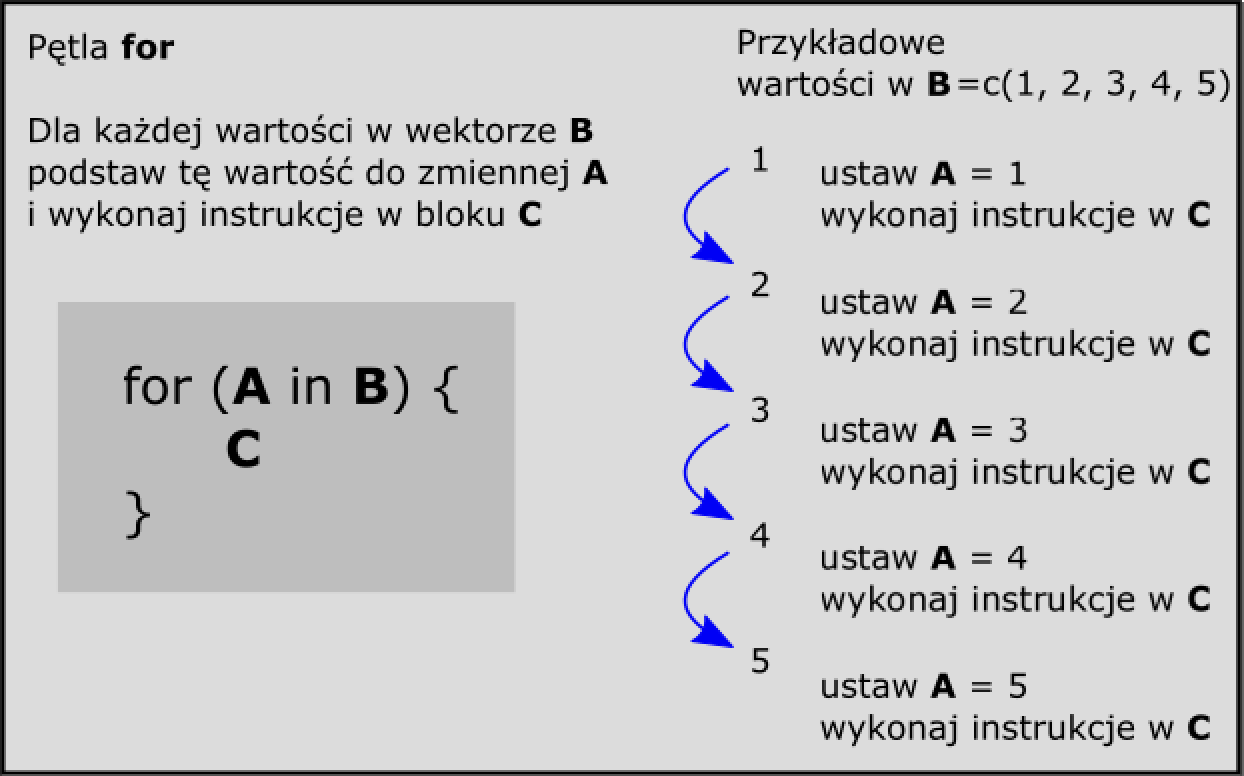
\includegraphics{figures/petla_pogromcy.png} \label{fig:petla}

\emph{Ciekawostka:} Teoretycznie kod instrukcji pętli można umieścić w
jednym ciągu, w tej samej linii co komendę \texttt{for}, np.:

\texttt{for(zmienna\ in\ 1:4)\ print(zmienna)}

Jednak bardziej czytelny zapis z blokiem pomiędzy nawiasami klamrowymi
sprawia, że schemat jednolinijkowy jest stosunkowo rzadko stosowany.

\subsection{Zadania treningowe - część
I}\label{zadania-treningowe---czesc-i}

\begin{enumerate}
\def\labelenumi{\arabic{enumi}.}
\tightlist
\item
  Napisz pętlę, która wyświetli napis \emph{R jest (tu wstaw dowolne
  słowo\ldots{})} 100 razy
\item
  Napisz pętlę, która za pomocą funkcji \texttt{sample()} ``puści kupon
  totolotka'' 10 razy. Jeśli brakuje wyniku postaraj się wymusić
  wyświetlenie stworzonej instrukcji za pomocą funkcji \texttt{print()}
\item
  Napisz pętlę wyświetlającą zmienną \texttt{i} o wartościach 3.5, 5 i
  20. Pamiętaj, że wartości definiowane po słowie kluczowym \texttt{in}
  również są wektorem!
\end{enumerate}

\begin{center}\rule{0.5\linewidth}{\linethickness}\end{center}

\subsection{Zadania treningowe - część
II}\label{zadania-treningowe---czesc-ii}

Pętla \texttt{for} może być wykorzystana nie tylko w przykładach
teoretycznych, ale także w praktyce\ldots{} Wyobraźmy sobie, że chcemy
wykonać wykres liniowy średniej miesięcznej temperatury powietrza w
Polsce dla określonego miesiąca w latach 1971-2000.

Wykonaj poniższe kroki:

\begin{enumerate}
\def\labelenumi{\arabic{enumi}.}
\tightlist
\item
  Wczytaj do obiektu \texttt{dane} zbiór danych znajdujący się pod
  adresem: \url{http://enwo.pl/przetwarzanie/dane/pl1.csv}
\item
  Wykres w najprostszej formie w \textbf{R} można wykonać za pomocą
  funkcji \texttt{plot()}, gdzie jako argumenty parametrów \texttt{x}
  oraz \texttt{y} należy podać wektory wartości położenia punktów na
  osiach x i y. Dodatkowo warto wykorzystać argument
  \texttt{type=\textquotesingle{}b\textquotesingle{}}, który połączy
  punkty (domyślny rodzaj wykresu) liniami. Wykonaj wykres dla stycznia.
  W razie konieczności skorzystaj z systemu pomocy dla funkcji
  \texttt{plot()}
\item
  Powtórz krok 2. wykonując wykres dla lutego. Dopisz dla funkcji
  \texttt{plot()} argument main=``2''
\item
  Korzystając z systemu pomocy zoptymalizuj wykres tak, aby zawierał
  poprawne podpisy osi x i y
\item
  \ldots{} \textbf{Za pomocą pętli \texttt{for} napisz kod, który
  stworzy wykresy dla wszystkich 12-tu miesięcy}
\end{enumerate}

\begin{verbatim}
## Warning in title(...): conversion failure on 'Styczeń - (1971-2000)' in
## 'mbcsToSbcs': dot substituted for <c5>
\end{verbatim}

\begin{verbatim}
## Warning in title(...): conversion failure on 'Styczeń - (1971-2000)' in
## 'mbcsToSbcs': dot substituted for <84>
\end{verbatim}

\begin{figure}

{\centering 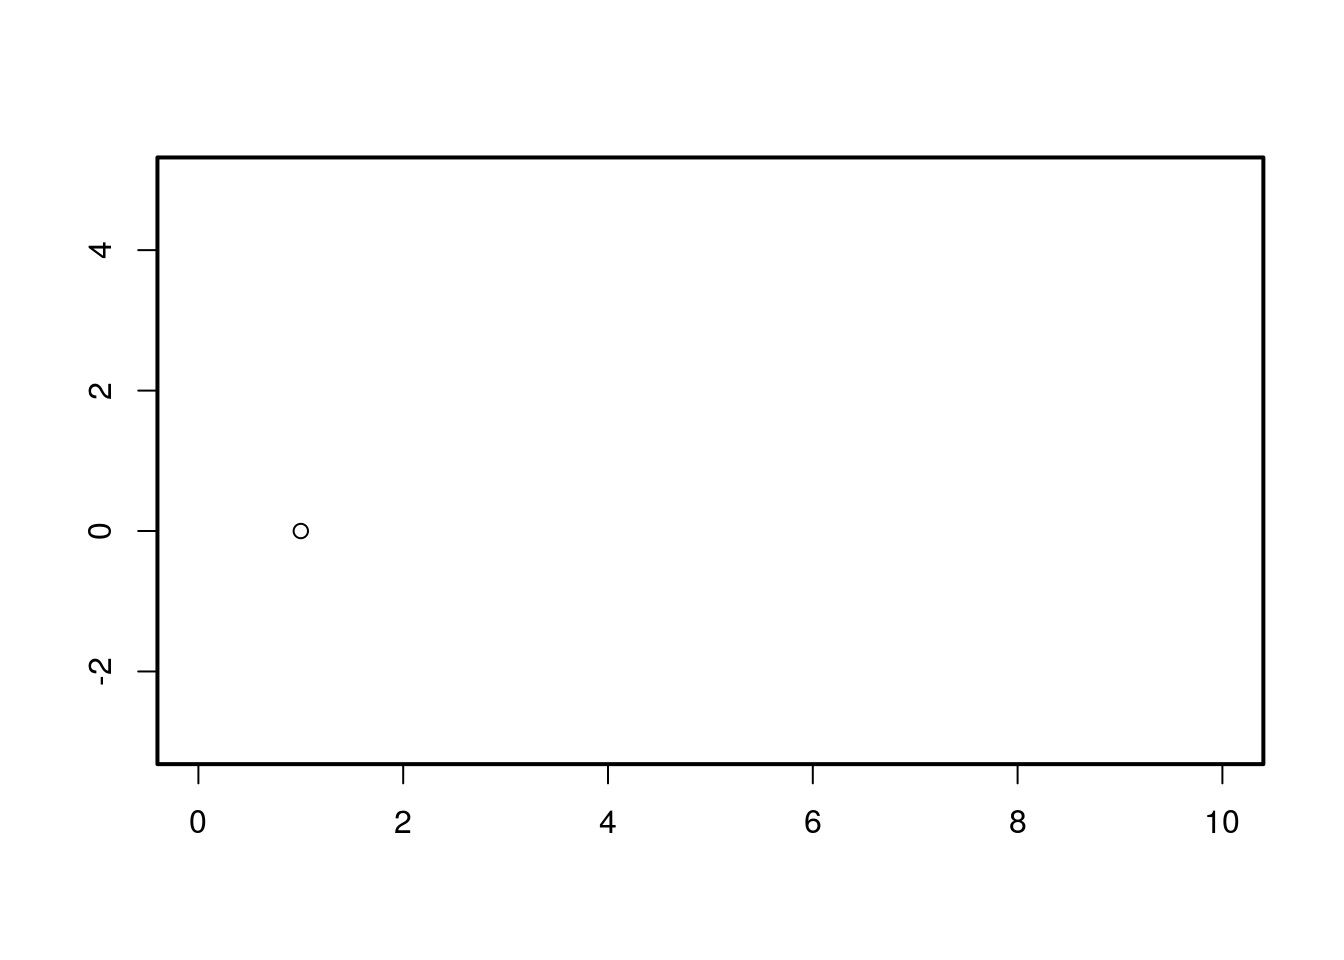
\includegraphics[width=0.8\linewidth]{ksiazka_files/figure-latex/unnamed-chunk-3-1} 

}

\caption{Temperatura stycznia w Polsce, 1971-2000}\label{fig:unnamed-chunk-3}
\end{figure}

\begin{enumerate}
\def\labelenumi{\arabic{enumi}.}
\setcounter{enumi}{5}
\tightlist
\item
  Jak w punkcie 5., ale zamiast wykresów stwórz histogramy oraz wyświetl
  w konsoli wynik dla średniej miesięcznej temperatury powietrza
\end{enumerate}

\subsection{Pętla w pętli}\label{petla-w-petli}

Często spotykanym zwyczajem (choć z początku małointuicyjnym) jest
zagnieżdżanie pętli. Dla czytelności kodu niektóre programy (jak np.
\textbf{RStudio}) automatycznie stosują tzw. wcięcia

Sprawdź działanie poniższego kodu, który wygeneruje wszelkie możliwe
kombinacje nazw stacji, lat i miesięcy w latach 2016-2017:

\begin{verbatim}
for(stacja in c("Poznań", "Łeba")){
  for(rok in c(2016,2017)){
    for(miesiac in 1:12){
    
    calosc <- paste(stacja, rok, miesiac) # funkcja paste "zlacza" ciagi tekstowe 
    print(calosc)
    
    } # ten nawias domyka petle dla zmiennej `miesiac`
  } # ten nawias domyka petle dla zmiennej `rok`
} # ten nawias domyka petle dla zmiennej `stacja`
\end{verbatim}

\subsection{Wykorzystanie pętli for do pobierania
danych}\label{wykorzystanie-petli-for-do-pobierania-danych}

Wiele danych meteorologicznych można pobrać za darmo z internetu. Dane
te są często w bardzo różnych formatach danych, dlatego najczęściej aby
móc na nich pracować należy je pobrać na dysk.

Jednym z najczęściej pobieranych zbiorów danych są reanalizy
meteorologicze NCEP/NCAR \citep{kalnay1996}
(\url{https://scholar.google.pl/citations?user=hLLKbYIAAAAJ\&hl=en\&oi=sra}).
Dane te można pobrać jako oddzielne pliki dla poszczególnych elementów
ze strony:
\url{ftp://ftp.cdc.noaa.gov/Datasets/ncep.reanalysis.dailyavgs/surface/}

Każdy z plików z danymi jest zapisany jako
\textbf{NAZWA\_PARAMETRU.ROK.nc}. Znając ten schemat nazywania plików
możemy pobrać dane np. dla temperatury powietrza (\emph{air.sig})
kopiując do schowka cały adres do pierwszego pliku
(\url{ftp://ftp.cdc.noaa.gov/Datasets/ncep.reanalysis.dailyavgs/surface/air.sig995.1948.nc})
i próbując za każdym razem podstawić w tym adresie zamiast liczby 1948
lata (liczby) które chcemy pobrać. Pobranie pliku w \textbf{R} umożliwia
funkcja \texttt{download.file()}. Z kolei do łączenia nazw użyjemy
funkcji \texttt{paste()}.

\begin{Shaded}
\begin{Highlighting}[]
\CommentTok{# 1) sprobujmy zlaczyc ciag tekstowy dla pobieranego adresu:}

\CommentTok{# pierwsza czesc adresu:}
\NormalTok{adres1 <-}\StringTok{ "ftp://ftp.cdc.noaa.gov/Datasets/ncep.reanalysis.dailyavgs/surface/air.sig995."}
\NormalTok{rok <-}\StringTok{ }\DecValTok{2016} \CommentTok{# jakis rok, ktory chcemy pobrac}
\NormalTok{adres2 <-}\StringTok{ ".nc"} \CommentTok{# dolaczanie koncowki adresu}

\NormalTok{link <-}\StringTok{ }\KeywordTok{paste}\NormalTok{(adres1,rok,adres2) }\CommentTok{# zlaczamy adres do finalnej postaci:}
\NormalTok{link}
\end{Highlighting}
\end{Shaded}

\begin{verbatim}
## [1] "ftp://ftp.cdc.noaa.gov/Datasets/ncep.reanalysis.dailyavgs/surface/air.sig995. 2016 .nc"
\end{verbatim}

\begin{Shaded}
\begin{Highlighting}[]
\CommentTok{# Ooopss...}
\CommentTok{# Okazuje sie, ze domyslnie funkcja paste() stosuje spacje pomiedzy }
\CommentTok{# zlaczanymi ciagami tekstu. Mozna to zmienic za pomoca opcji 'sep'}

\NormalTok{link <-}\StringTok{ }\KeywordTok{paste}\NormalTok{(adres1,rok,adres2, }\DataTypeTok{sep=}\StringTok{""}\NormalTok{) }\CommentTok{# poprawiamy link aby nie mial spacji}
\NormalTok{link}
\end{Highlighting}
\end{Shaded}

\begin{verbatim}
## [1] "ftp://ftp.cdc.noaa.gov/Datasets/ncep.reanalysis.dailyavgs/surface/air.sig995.2016.nc"
\end{verbatim}

\begin{Shaded}
\begin{Highlighting}[]
\CommentTok{# 2) Skoro nazwa jest poprawna sprobujmy uzyc funkcji download.file() }
\CommentTok{#    do pobrania wygenerowanego linku. Musimy dodatkowo wygenerowac nazwe}
\CommentTok{#    pliku, ktory bedzie zapisany na dysku}

\NormalTok{plik <-}\StringTok{ }\KeywordTok{paste}\NormalTok{(rok,adres2,}\DataTypeTok{sep=}\StringTok{""}\NormalTok{)}
\end{Highlighting}
\end{Shaded}

\textbf{Zadanie treningowe/domowe:}

\begin{enumerate}
\def\labelenumi{\arabic{enumi}.}
\tightlist
\item
  Korzystając z pętli \texttt{for} pobierz pliki dla temperatury
  powietrza z reanaliz NCEP/NCAR dla lat 2016-2010
\item
  W linku: enwo.pl/przetwarzanie/dane/pl2013.zip zapisano dane
  meteorologiczne dla głównych polskich stacji meteorologicznych z roku
  2013. Rozpakuj te dane na dysku a następnie napisz pętlę
  programistyczną która: 2.1. Wczyta te pliki do \textbf{R} (przydatne
  może być przekazanie wyniku funkcji \texttt{dir()} do zmiennej) 2.2.
  Wyświetli średnią arytmetyczną z wartości zapisanych w drugiej
  kolumnie w każdym z plików
\end{enumerate}

\section{\texorpdfstring{Pętla
\emph{while}}{Pętla while}}\label{petla-while}

Kolejną pętlą, nieco rzadziej stosowaną, jest pętla \texttt{while}.
Wykonuje się ona tak długo, aż testowany warunek logiczny przestanie
zwracać wartość \texttt{TRUE}. W niektórych przypadkach takie
rozwiązanie może powodać potencjalne zagrożenie, gdyż pętla może działać
w nieskończoność.

Ogólna postać pętli \texttt{while} wygląda bardzo podobnie do pętli
\texttt{for}, z tą różnicą że w nawiasie testowany jest warunek
logiczny, a w przypadku testowania warunku logicznego na zmiennych muszą
one być zadeklarowane przed instrukcją \texttt{while}.

Sprawdźmy to na przykładzie:

\begin{Shaded}
\begin{Highlighting}[]
\NormalTok{zmienna <-}\StringTok{ }\DecValTok{1}
\ControlFlowTok{while}\NormalTok{(zmienna}\OperatorTok{>}\DecValTok{0}\NormalTok{)\{        }\CommentTok{# sprawdz warunek logiczny, czy zmienna jest > 0}
                         \CommentTok{# jesli tak, to uruchom to co jest pomiedzy \{\}}
  
  \KeywordTok{print}\NormalTok{(zmienna)         }\CommentTok{# wyswietlam aktualna wartosc zmiennej}
\NormalTok{  zmienna <-}\StringTok{ }\NormalTok{zmienna}\FloatTok{-0.3} \CommentTok{# zmniejszam wartosc zmiennej o 0.3}
\NormalTok{\}}
\end{Highlighting}
\end{Shaded}

\begin{verbatim}
## [1] 1
## [1] 0.7
## [1] 0.4
## [1] 0.1
\end{verbatim}

Pętla została uruchomiona 4 razy ponieważ za pierwszym razem przy
testowaniu warunku logicznego zmienna miała wartość 1 i zmniejszała się
aż do 0.1, po czym przy ostatnim uruchomieniu pętli zmienna otrzymała
wartość -0.2 i warunek logicznych \texttt{zmienna\textgreater{}0}
zapisany w instrukcji \texttt{while} dał wartość \texttt{FALSE} i pętla
zaprzestała swojego działania.

\subsection{\texorpdfstring{Przykład z pętlą
\emph{while}}{Przykład z pętlą while}}\label{przykad-z-petla-while}

Zagrajmy z komputerem w totolotka.

\begin{enumerate}
\def\labelenumi{\arabic{enumi}.}
\tightlist
\item
  Wybierz wektor 6 unikalnych wartości w przedziale od 1 do 49. Zapisz
  wynik do obiektu \texttt{kupon}
\item
  Wylosuj 6 liczb z rozkładu jednostajnego płaskiego za pomocą funkcji
  \texttt{sample()} i zapisz wynik do obiektu \texttt{wynik}
\item
  Sprawdź czy wygrałeś poprzez działanie w krokach 4-6:
\item
  Dokonaj konkatenacji obiektów \texttt{wynik} i \texttt{kupon} do
  obiektu \texttt{razem}
\item
  Sprawdź za pomocą funkcji \texttt{duplicated()} czy obiekt
  \texttt{razem} zawiera \textgreater{}2 powtórzenia. Wynik funkcji
  \texttt{duplicated()} daje wartości logiczne, które można zsumować
  (TRUE = 1, FALSE = 0)
\item
  Zapisz wynik otrzymany w poprzednim punkcie do zmiennej
  \texttt{wygrana}
\item
  Całe postępowanie wprowadź do pętli \texttt{while}, która będzie się
  uruchamiać tak długo, aż nie wygrasz (tzn. trafisz choć 3 liczby)
\item
  \ldots{} Policz czy kto wygrał \ldots{}
\end{enumerate}

Przykładowe rozwiązanie:

\begin{Shaded}
\begin{Highlighting}[]
\NormalTok{nr_zakladu <-}\StringTok{ }\DecValTok{0}  \CommentTok{# sprawdzmy ile totolotkow musimy puscic zanim wygramy chocby 'trojke'}
\NormalTok{kupon <-}\StringTok{ }\KeywordTok{c}\NormalTok{(}\DecValTok{10}\NormalTok{, }\DecValTok{17}\NormalTok{, }\DecValTok{23}\NormalTok{, }\DecValTok{26}\NormalTok{, }\DecValTok{39}\NormalTok{, }\DecValTok{49}\NormalTok{)}
\NormalTok{wygrana <-}\StringTok{ }\DecValTok{0}
\ControlFlowTok{while}\NormalTok{(wygrana}\OperatorTok{<}\DecValTok{3}\NormalTok{)\{ }\CommentTok{# jesli bedzie >= 3 to znaczy ze wygralismy, }
                   \CommentTok{# w przeciwnym razie gramy jeszcze raz}
\NormalTok{  wynik <-}\StringTok{ }\KeywordTok{sample}\NormalTok{(}\DecValTok{1}\OperatorTok{:}\DecValTok{49}\NormalTok{, }\DecValTok{6}\NormalTok{)}
\NormalTok{  razem <-}\StringTok{ }\KeywordTok{c}\NormalTok{(wynik, kupon)}
\NormalTok{  wygrana <-}\StringTok{ }\KeywordTok{sum}\NormalTok{(}\KeywordTok{duplicated}\NormalTok{(razem))}
  
\NormalTok{  nr_zakladu <-}\StringTok{ }\NormalTok{nr_zakladu }\OperatorTok{+}\DecValTok{1}
  
  \KeywordTok{cat}\NormalTok{(}\KeywordTok{c}\NormalTok{(nr_zakladu,}\StringTok{"wylosowane liczby to:"}\NormalTok{, wynik,}\StringTok{"}\CharTok{\textbackslash{}n}\StringTok{"}\NormalTok{))}
\NormalTok{\}}
\end{Highlighting}
\end{Shaded}

\begin{verbatim}
## 1 wylosowane liczby to: 14 18 27 42 10 40 
## 2 wylosowane liczby to: 47 32 30 3 10 8 
## 3 wylosowane liczby to: 34 19 37 23 33 44 
## 4 wylosowane liczby to: 19 38 44 10 30 6 
## 5 wylosowane liczby to: 14 19 1 18 40 15 
## 6 wylosowane liczby to: 24 29 49 9 38 30 
## 7 wylosowane liczby to: 39 6 35 19 37 29 
## 8 wylosowane liczby to: 39 27 25 37 2 21 
## 9 wylosowane liczby to: 36 34 23 40 20 11 
## 10 wylosowane liczby to: 4 5 15 24 30 18 
## 11 wylosowane liczby to: 45 15 22 16 30 12 
## 12 wylosowane liczby to: 24 37 4 41 16 48 
## 13 wylosowane liczby to: 17 49 23 42 39 18
\end{verbatim}

\subsection*{Zadanie domowe}\label{zadanie-domowe-3}
\addcontentsline{toc}{subsection}{Zadanie domowe}

\subsubsection*{Pętla while - pobierz dane
IMGW-PIB}\label{petla-while---pobierz-dane-imgw-pib}
\addcontentsline{toc}{subsubsection}{Pętla while - pobierz dane
IMGW-PIB}

Na stronie \url{https://dane.imgw.pl/} istnieje możliwość pobrania
danych meteorologicznych ze zbiorów IMGW-PIB. Jednorazowo można pobrać z
poziomu przeglądarki tylko fragment całości udostępionych danych.
Pobieranie danych dla dłuższych okresów czasu wymagałoby żmudnej i
czasochłonnej pracy, stąd też można do tego celu wykorzystać dowolną
pętlę programistyczną i funkcję \texttt{download.file()}. Dla ułatwienia
działania kod automatyzujący pobieranie danych zapisano w postaci
pakietu \texttt{imgw} dostępnego na stronie
\url{http://github.com/bczernecki/imgw} . W celu sprawdzenia działania
niniejszego rozwiązania wykonaj poniższe polecenia:

\begin{enumerate}
\def\labelenumi{\arabic{enumi}.}
\tightlist
\item
  Zainstaluj i następnie aktywuj pakiet \texttt{devtools}. Pozwola on na
  instalowanie także nieoficjalnych paczek R.
\item
  Za pomocą instrukcji \texttt{install\_github("bczernecki/imgw")}
  zainstaluj pakiet nazwany \texttt{imgw} i następnie go aktywuj.
\item
  Zapoznaj się z dokumentacją do tego pakietu i pobierz przykładowe dane
  meteorologiczne.
\item
  Przeanalizuj kod wpisując w konsoli samą nazwę funkcji pobierającej
  (tj. \texttt{pobierz} - bez nawiasów i argumentów). Sprawdź sposób
  działania funkcji który wyświetli się w konsoli. Utwórz nowy skrypt i
  sprawdzaj działanie kodu funkcji \texttt{pobierz} uruchamiając
  poszczególne instrukcje linia po linii. Unikaj pętli w celu lepszego
  zrozumienia sposobu działania kodu.
\end{enumerate}

\subsection*{Zadanie sprawdzające}\label{zadanie-sprawdzajace-1}
\addcontentsline{toc}{subsection}{Zadanie sprawdzające}

\chapter{Czas i napisy}\label{czas-i-napisy}

W meteorologii i klimatologii niezmiernie ważne jest analizowanie
zbiorów danych w aspekcie czasowym. Przed rozpoczęciem analizy szeregów
czasowych niezbędne jest zrozumienie sposobu przechowywania tego typu
danych przez komputer.

W \textbf{R} powszechnie stosowane są 2-3 formaty przechowywania czasu:

\begin{itemize}
\item
  Klasa \texttt{Date} - wystarczająca jeśli nie mamy danych o
  rozdzielczości mniejszej niż dobowa (\emph{sub-daily}) oraz nasze dane
  nie wymagają różnic w zmianach czasu urzędowego
\item
  Klasy POSIX-owe: \texttt{POSIXct} oraz \texttt{POSIXlt} (odpowiednio:
  \emph{calendar} i \emph{local time}). Zdecydowanie częściej stosowana
  jest klasa \texttt{POSIXct}, która pozwala na przechowywanie czasu z
  dokładnością do sekundy (lub jej części ułamkowych). Poza tym
  obsługuje kwestie problematyczne związane z różnymi strefami czasowymi
  oraz zmianą czasu.
\end{itemize}

\section{Date}\label{date}

Konstruktorem klasy Date jest funkcja \texttt{as.Date()}.

Jako pierwszy argument przyjmuje wektor napisów opisujących daty. Drugi
opcjonalny argument określa formatowanie daty. Domyślne formatowanie to
rok-miesiąc-dzień.

\begin{Shaded}
\begin{Highlighting}[]
\KeywordTok{as.Date}\NormalTok{(}\StringTok{"2015-02-22"}\NormalTok{)}
\end{Highlighting}
\end{Shaded}

\begin{verbatim}
## [1] "2015-02-22"
\end{verbatim}

Jeśli chcemy zmienić sposób deklarowania daty możemy użyc argumentu
\texttt{format}

\begin{Shaded}
\begin{Highlighting}[]
\KeywordTok{as.Date}\NormalTok{(}\StringTok{"02/22/2015"}\NormalTok{, }\DataTypeTok{format =} \StringTok{"%m/%d/%Y"}\NormalTok{)}
\end{Highlighting}
\end{Shaded}

\begin{verbatim}
## [1] "2015-02-22"
\end{verbatim}

Aby uzyskać dokładną pomoc dotyczącą oznaczeń w formatowaniu daty należy
otworzyć plik pomocy instrukcją \texttt{?strptime}.

Obiekty klasy Date można tworzyć także na podstawie liczb całkowitych
lub obiektów klasy POSIXct, w obu przypadkach przy pomocy funkcji
\texttt{as.Date()}.

\subsection*{Zadanie sprawdzające}\label{zadanie-sprawdzajace-2}
\addcontentsline{toc}{subsection}{Zadanie sprawdzające}

\begin{enumerate}
\def\labelenumi{\arabic{enumi}.}
\tightlist
\item
  Utwórz dowolnie nazwany obiekt przechowujący dzisiejszą datę
\item
  Dodaj lub odejmij od niego dowolną liczbę całkowitą oraz wektor w
  postaci sekwencji liczb wygenerowanych za pomocą operatora \texttt{:}
\item
  W \textbf{R} daty przechowywane są również jako liczby. Sprawdź
  działanie funkcji \texttt{as.numeric()} na dowolnym obiekcie klasy
  Date. Jaki dzień to dla komputera 0?
\end{enumerate}

\subsection{W jaki sposób najszybciej utworzyć ciąg
dat?}\label{w-jaki-sposob-najszybciej-utworzyc-ciag-dat}

Bardzo często zdarza się, że konieczne jest wygenerowanie ciągu dat,
które będziemy umieszczać w jednej z kolumn ramki danych. Podobnie jak w
przypadku ``normalnych'' wektorów również do tego celu możemy zastosować
funkcję \texttt{seq}, która w przypadku operacji na datach ma także
postać rozszerzoną jako \texttt{seq.Date()}. Sprawdź pomoc dla tej
funkcji. Następnie:

\begin{enumerate}
\def\labelenumi{\arabic{enumi}.}
\tightlist
\item
  Utwórz datę początkową i końcową dla generowanego ciągu dat:
\end{enumerate}

\begin{Shaded}
\begin{Highlighting}[]
\NormalTok{poczatek <-}\StringTok{ }\KeywordTok{as.Date}\NormalTok{(}\StringTok{"2016-01-01"}\NormalTok{)}
\NormalTok{koniec <-}\StringTok{ }\KeywordTok{as.Date}\NormalTok{(}\StringTok{"2016-12-31"}\NormalTok{)}
\end{Highlighting}
\end{Shaded}

\begin{enumerate}
\def\labelenumi{\arabic{enumi}.}
\setcounter{enumi}{1}
\tightlist
\item
  Podłącz wygenerowane obiekty jako argumenty \texttt{from} oraz
  \texttt{to} dla funkcji \texttt{seq.Date()} oraz opcję \texttt{by}
  jako dzień (ang. \emph{day}):
\end{enumerate}

\begin{Shaded}
\begin{Highlighting}[]
\NormalTok{naszedaty <-}\StringTok{ }\KeywordTok{seq.Date}\NormalTok{(}\DataTypeTok{from=}\NormalTok{poczatek, }\DataTypeTok{to=}\NormalTok{koniec, }\DataTypeTok{by=}\StringTok{"day"}\NormalTok{)}
\KeywordTok{head}\NormalTok{(naszedaty)}
\end{Highlighting}
\end{Shaded}

\begin{verbatim}
## [1] "2016-01-01" "2016-01-02" "2016-01-03" "2016-01-04" "2016-01-05"
## [6] "2016-01-06"
\end{verbatim}

\begin{enumerate}
\def\labelenumi{\arabic{enumi}.}
\setcounter{enumi}{2}
\tightlist
\item
  Czasem jednak niezbędne jest wygenerowanie dat w pewnych interwałach
  czasu, np. co tydzień, albo co kilka- kilkanaście dni. Do tego celu
  można użyć opcji \texttt{by}. Przykładowo, daty z interwałem co
  tydzień, można wygenerować wg jednej z poniższych opcji:
\end{enumerate}

\begin{Shaded}
\begin{Highlighting}[]
\NormalTok{cotydzien1 <-}\StringTok{ }\KeywordTok{seq.Date}\NormalTok{(}\DataTypeTok{from=}\NormalTok{poczatek, }\DataTypeTok{to=}\NormalTok{koniec, }\DataTypeTok{by=}\StringTok{"week"}\NormalTok{)}
\NormalTok{cotydzien2 <-}\StringTok{ }\KeywordTok{seq.Date}\NormalTok{(}\DataTypeTok{from=}\NormalTok{poczatek, }\DataTypeTok{to=}\NormalTok{koniec, }\DataTypeTok{by=}\StringTok{"7 days"}\NormalTok{)}
\KeywordTok{head}\NormalTok{(cotydzien1)}
\end{Highlighting}
\end{Shaded}

\begin{verbatim}
## [1] "2016-01-01" "2016-01-08" "2016-01-15" "2016-01-22" "2016-01-29"
## [6] "2016-02-05"
\end{verbatim}

\begin{Shaded}
\begin{Highlighting}[]
\KeywordTok{head}\NormalTok{(cotydzien2)}
\end{Highlighting}
\end{Shaded}

\begin{verbatim}
## [1] "2016-01-01" "2016-01-08" "2016-01-15" "2016-01-22" "2016-01-29"
## [6] "2016-02-05"
\end{verbatim}

\subsection{Operowanie datami}\label{operowanie-datami}

Wiele operacji na datach nie należy do trywialnych lub intuicyjnych.
Przykładowo, jeśli chcemy \emph{wyciągnać} z obiektu klasy Date jaki to
jest dzień tygodnia możemy posłużyć się opcją formatowania opisaną w
systemie pomocy pod hasłem \texttt{?strptime}. Sprawdźmy na przykładzie
dla obiektu \texttt{naszedaty}:

\begin{Shaded}
\begin{Highlighting}[]
\NormalTok{dnitygodnia <-}\StringTok{ }\KeywordTok{format}\NormalTok{(naszedaty,}\StringTok{"%A"}\NormalTok{) }
\KeywordTok{head}\NormalTok{(dnitygodnia)}
\end{Highlighting}
\end{Shaded}

\begin{verbatim}
## [1] "Friday"    "Saturday"  "Sunday"    "Monday"    "Tuesday"   "Wednesday"
\end{verbatim}

\subsection{\texorpdfstring{Biblioteka
\texttt{lubridate}}{Biblioteka lubridate}}\label{biblioteka-lubridate}

Znaczna część operacji na datach jest usprawniona dzięki pakietom
\textbf{R}, dedykowanym do pracy na obiektach zawierających czas. Jednym
z nich jest biblioteka \texttt{lubridate}. Aby z niej korzystać należy
ją zainstalować i aktywować.

\begin{Shaded}
\begin{Highlighting}[]
\CommentTok{#install.packages("lubridate") # jesli nie byl wczesniej zainstalowany}
\KeywordTok{library}\NormalTok{(lubridate)}
\end{Highlighting}
\end{Shaded}

\begin{verbatim}
## 
## Attaching package: 'lubridate'
\end{verbatim}

\begin{verbatim}
## The following object is masked from 'package:base':
## 
##     date
\end{verbatim}

Przyjrzyjmy się działaniu przykładowych funkcji z tego pakietu:

\begin{Shaded}
\begin{Highlighting}[]
\KeywordTok{now}\NormalTok{()}
\end{Highlighting}
\end{Shaded}

\begin{verbatim}
## [1] "2018-06-21 21:42:51 CEST"
\end{verbatim}

\begin{Shaded}
\begin{Highlighting}[]
\KeywordTok{today}\NormalTok{()}
\end{Highlighting}
\end{Shaded}

\begin{verbatim}
## [1] "2018-06-21"
\end{verbatim}

\begin{Shaded}
\begin{Highlighting}[]
\NormalTok{dzis <-}\StringTok{ }\KeywordTok{today}\NormalTok{()}

\KeywordTok{week}\NormalTok{(dzis)}
\end{Highlighting}
\end{Shaded}

\begin{verbatim}
## [1] 25
\end{verbatim}

\begin{Shaded}
\begin{Highlighting}[]
\KeywordTok{day}\NormalTok{(dzis)}
\end{Highlighting}
\end{Shaded}

\begin{verbatim}
## [1] 21
\end{verbatim}

\begin{Shaded}
\begin{Highlighting}[]
\KeywordTok{month}\NormalTok{(dzis)}
\end{Highlighting}
\end{Shaded}

\begin{verbatim}
## [1] 6
\end{verbatim}

\begin{Shaded}
\begin{Highlighting}[]
\KeywordTok{months}\NormalTok{(dzis)}
\end{Highlighting}
\end{Shaded}

\begin{verbatim}
## [1] "June"
\end{verbatim}

\begin{Shaded}
\begin{Highlighting}[]
\KeywordTok{year}\NormalTok{(dzis)}
\end{Highlighting}
\end{Shaded}

\begin{verbatim}
## [1] 2018
\end{verbatim}

\subsection*{Zadanie}\label{zadanie}
\addcontentsline{toc}{subsection}{Zadanie}

\begin{enumerate}
\def\labelenumi{\arabic{enumi}.}
\tightlist
\item
  Oblicz ile dni trwała druga wojna światowa w Europie (1. września 1945
  - 8 maja 1945).
\item
  Sprawdź jaki dzień tygodnia będzie za 100 dni od dziś
\end{enumerate}

\section{POSIXct}\label{posixct}

Konstruktorem klasy POSIXct jest funkcja \texttt{as.POSIXct()}. Jako
pierwszy argument przyjmuje wektor napisów opisujących chwile czasu.
Drugi opcjonalny argument określa formatowanie daty. Domyślne
formatowanie to rok-miesiąc-dzień godzina:minuta:sekunda.

Aby uzyskać dokładną pomoc dotyczącą oznaczeń w formatowaniu daty należy
otworzyć plik pomocy instrukcją ?strptime.

\begin{Shaded}
\begin{Highlighting}[]
\NormalTok{czas1 <-}\StringTok{ }\KeywordTok{as.POSIXct}\NormalTok{(}\StringTok{"2015-02-13 12:56:26"}\NormalTok{)}
\NormalTok{czas1}
\end{Highlighting}
\end{Shaded}

\begin{verbatim}
## [1] "2015-02-13 12:56:26 CET"
\end{verbatim}

\begin{Shaded}
\begin{Highlighting}[]
\NormalTok{czas2 <-}\StringTok{ }\KeywordTok{as.POSIXct}\NormalTok{(}\StringTok{"14022015 12:56:26"}\NormalTok{, }\DataTypeTok{format =} \StringTok{"%d%m%Y %H:%M:%S"}\NormalTok{)}
\NormalTok{czas2}
\end{Highlighting}
\end{Shaded}

\begin{verbatim}
## [1] "2015-02-14 12:56:26 CET"
\end{verbatim}

Na czasach można wykonywać takie operacje jak odejmowanie czy dodawane
do określonego przedziału czasu (dodanie liczby całkowitej, domyślnie
dodaje określoną liczbę sekund).

\begin{Shaded}
\begin{Highlighting}[]
\NormalTok{czas2 }\OperatorTok{-}\StringTok{ }\NormalTok{czas1}
\end{Highlighting}
\end{Shaded}

\begin{verbatim}
## Time difference of 1 days
\end{verbatim}

Możemy także sprawdzić lub nadać właściwości związane ze strefą czasową:

\begin{Shaded}
\begin{Highlighting}[]
\KeywordTok{tz}\NormalTok{(czas2)}
\end{Highlighting}
\end{Shaded}

\begin{verbatim}
## [1] ""
\end{verbatim}

\ldots{} choć niektóre rzeczy łatwiej zrobić za pomocą klasycznych
instrukcji POSIXowych. Sprawdźmy różnicę czasu pomiędzy Jerozolimą i
Warszawą w dn. 21 czerwca:

\begin{Shaded}
\begin{Highlighting}[]
\NormalTok{warszawa <-}\StringTok{ }\KeywordTok{as.POSIXct}\NormalTok{(}\StringTok{"2017-06-21 16:00:00"}\NormalTok{, }\DataTypeTok{tz =} \StringTok{"Europe/Warsaw"}\NormalTok{)}
\NormalTok{jerozolima <-}\StringTok{  }\KeywordTok{as.POSIXct}\NormalTok{(}\StringTok{"2017-06-21 16:00:00"}\NormalTok{, }\DataTypeTok{tz =} \StringTok{"Asia/Jerusalem"}\NormalTok{)}
\NormalTok{jerozolima}\OperatorTok{-}\NormalTok{warszawa}
\end{Highlighting}
\end{Shaded}

\begin{verbatim}
## Time difference of -1 hours
\end{verbatim}

\subsection*{Zadanie domowe}\label{zadanie-domowe-4}
\addcontentsline{toc}{subsection}{Zadanie domowe}

\begin{enumerate}
\def\labelenumi{\arabic{enumi}.}
\tightlist
\item
  Wczytaj plik z danymi dostępnymi na stronie
  \url{http://enwo.pl/przetwarzanie/dane/poz.txt} .
\item
  Następnie przekonwertuj kolumnę/kolumny reprezentujące czas na nową
  kolumnę zawierającą czas jako obiekt klasy \texttt{Date}. Możesz także
  utworzyć więcej nowych kolumn w zależności od własnych potrzeb.
\item
  Oblicz średnią wartość temperatury dla wybranego (jednego miesiąca).
\end{enumerate}

\subsection*{Zadanie podsumowujące}\label{zadanie-podsumowujace}
\addcontentsline{toc}{subsection}{Zadanie podsumowujące}

TBA

\chapter{dplyr - część I}\label{dplyr---czesc-i}

Wiele operacji wykonywanych na ramkach danych ma bardzo podobną
strukturę. Bardzo często zbiory danych łączymy, filtrujemy, rozdzielamy,
grupujemy, obliczamy wybrane statystyki i wizualizujemy w poszukiwaniu
istoty problemu. Wiele z tych operacji wykonywanych na ramkach danych
można wykorzystać za pomocą natywnie dostępnych funkcji \textbf{R}.
Można także skorzystać z kilku-, kilkunastu pakietów bardzo popularnych
wśród analityków danych, które skracają czas obliczeń o 80\% i pozwalają
na zawarcie istoty problemu w zaledwie kilku liniach kodu\ldots{}

Jedną z najczęściej wykorzystywanych bibliotek do analizy danych jest
biblioteka \texttt{dplyr} \citep{dplyr2016}, która w dużym stopniu
zrewolucjonizowała analizę danych w środowisku \textbf{R}. Poniżej
zostanie przedstawionych kilka praktycznych przykładów związanych z
wykorzystaniem wybranych funkcji z tego pakietu.

\emph{Pakiet \texttt{dplyr} nie jest dostępny w domyślnym środowisku
\textbf{R}, stąd też wymagana jest jego wcześniejsza, jednorazowa
instalacja oraz aktywacja.}

\section{\texorpdfstring{Łączenie ramek danych -
\texttt{left\_join()}}{Łączenie ramek danych - left\_join()}}\label{aczenie-ramek-danych---left_join}

Do połączenia dwóch ramek danych na podstawie wspólnego identyfikatora
można użyć natywnie dostępnej w \textbf{R} funkcji \texttt{merge()} lub
skorzystać z jednej z odmian funkcji \texttt{join} dostępnej w
bibliotece \texttt{dplyr}. Najczęściej stosowana komenda to
\texttt{left\_join()}, która zwraca wszystkie elementy z pierwszej ramki
danych oraz wszystkie kolumny z obu łączonych ramek danych.

Spójrzmy na schemat działania tej funkcji na podstawie poniższego
przykładu z dwiema ramkami danych zawierających

\begin{Shaded}
\begin{Highlighting}[]
\NormalTok{df1 <-}\StringTok{ }\KeywordTok{data.frame}\NormalTok{(}\DataTypeTok{id_stacji =} \KeywordTok{c}\NormalTok{(}\DecValTok{1}\OperatorTok{:}\DecValTok{4}\NormalTok{,}\DecValTok{3}\NormalTok{), }\DataTypeTok{pomiar1 =} \KeywordTok{c}\NormalTok{(}\FloatTok{2.5}\NormalTok{,}\FloatTok{1.25}\NormalTok{,}\DecValTok{2}\NormalTok{,}\DecValTok{3}\NormalTok{,}\DecValTok{2}\NormalTok{))}
\NormalTok{df2 <-}\StringTok{ }\KeywordTok{data.frame}\NormalTok{(}\DataTypeTok{id_stacji =} \KeywordTok{c}\NormalTok{(}\DecValTok{1}\NormalTok{, }\DecValTok{3}\NormalTok{, }\DecValTok{5}\NormalTok{), }\DataTypeTok{pomiar2 =} \KeywordTok{c}\NormalTok{(}\FloatTok{10.2}\NormalTok{,}\FloatTok{9.6}\NormalTok{, }\FloatTok{12.3}\NormalTok{), }\DataTypeTok{inne =}\NormalTok{ letters[}\DecValTok{1}\OperatorTok{:}\DecValTok{3}\NormalTok{])}
\KeywordTok{print}\NormalTok{(df1)}
\end{Highlighting}
\end{Shaded}

\begin{verbatim}
##   id_stacji pomiar1
## 1         1    2.50
## 2         2    1.25
## 3         3    2.00
## 4         4    3.00
## 5         3    2.00
\end{verbatim}

\begin{Shaded}
\begin{Highlighting}[]
\KeywordTok{print}\NormalTok{(df2)}
\end{Highlighting}
\end{Shaded}

\begin{verbatim}
##   id_stacji pomiar2 inne
## 1         1    10.2    a
## 2         3     9.6    b
## 3         5    12.3    c
\end{verbatim}

Jeśli chcemy złączyć obie ramki danych: \texttt{df1} oraz \texttt{df2}
na podstawie kolumny \texttt{id\_stacji} najszybciej wynik działania
dostaniemy działając funkcją \texttt{left\_join()}:

\begin{Shaded}
\begin{Highlighting}[]
\KeywordTok{library}\NormalTok{(dplyr)}
\end{Highlighting}
\end{Shaded}

\begin{verbatim}
## 
## Attaching package: 'dplyr'
\end{verbatim}

\begin{verbatim}
## The following objects are masked from 'package:lubridate':
## 
##     intersect, setdiff, union
\end{verbatim}

\begin{verbatim}
## The following objects are masked from 'package:stats':
## 
##     filter, lag
\end{verbatim}

\begin{verbatim}
## The following objects are masked from 'package:base':
## 
##     intersect, setdiff, setequal, union
\end{verbatim}

\begin{Shaded}
\begin{Highlighting}[]
\KeywordTok{left_join}\NormalTok{(df1,df2)}
\end{Highlighting}
\end{Shaded}

\begin{verbatim}
## Joining, by = "id_stacji"
\end{verbatim}

\begin{verbatim}
##   id_stacji pomiar1 pomiar2 inne
## 1         1    2.50    10.2    a
## 2         2    1.25      NA <NA>
## 3         3    2.00     9.6    b
## 4         4    3.00      NA <NA>
## 5         3    2.00     9.6    b
\end{verbatim}

Jak widać na powyższym przykładzie funkcja domyślnie poszukała kolumny w
obu zbiorach danych o takiej samej nazwie i na tej podstawie dokonała
złączenia. Jednocześnie identyfikatory stacji, które nie istniały w
drugiej ramce danych zostały uzupełnione jako braki danych
(\texttt{NA}). \emph{Jeśli chcielibyśmy uzyskać inne możliwe kombinacje
możemy zastosować inne warianty rodziny funkcji join opisanej w systemie
pomocy \textbf{R} }

\subsubsection*{Brak wspólnej nazwy kolumny
łączącej}\label{brak-wspolnej-nazwy-kolumny-aczacej}
\addcontentsline{toc}{subsubsection}{Brak wspólnej nazwy kolumny
łączącej}

Funkcja \texttt{left\_join()} domyślnie szuka wspólnych nazw kolumn na
podstawie których łączy dwie ramki danych. Jeśli nazwy kolumn po których
chcemy dokonać złączenia są różne możemy:

\begin{itemize}
\tightlist
\item
  odpowiednio wcześniej zunifikować te nazwy (np. za pomocą
  \texttt{colnames()})
\item
  lub wskazać funkcji \texttt{left\_join()} argument \texttt{by=} z
  kolumnami po których chcemy złączać
\end{itemize}

W celu sprawdzenia takiego schematu postępowania pobierz dane z adresu
\url{http://enwo.pl/przetwarzanie/dane/przyklad1_join.Rdata} i załaduj
do środowiska \textbf{R}. W zakładce \emph{Environment} powinny pojawić
się 2 nowe obiekty:

\begin{itemize}
\tightlist
\item
  \texttt{xym} - zawiera współrzędne geograficzne, wysokości stacji,
  międzynarodowe kody stacji i nazwy stacji meteorologicznych
\item
  \texttt{wynik}- zawiera podsumowanie dobowe dla temperatury
  maksymalnej, minimalnej i średniej wg depesz SYNOP z godz. 6:00 UTC
\end{itemize}

\begin{Shaded}
\begin{Highlighting}[]
\KeywordTok{load}\NormalTok{(}\StringTok{"/home/bartosz/github/przetwarzanie/dane/przyklad1_join.Rdata"}\NormalTok{)}
\KeywordTok{head}\NormalTok{(xym)}
\end{Highlighting}
\end{Shaded}

\begin{verbatim}
##        lon      lat alt  code         name
## 1 27.95000 55.81667 133 26554 Verhnedvinsk
## 2 27.46667 55.36667 131 26643 Sarcovschina
## 3 26.31667 55.05000 209 26645      Lyntupy
## 4 28.76667 55.46667 133 26653       Polock
## 5 27.75000 54.88333 197 26657    Dokshitsy
## 6 28.70000 54.88333 174 26659        Lepel
\end{verbatim}

\begin{Shaded}
\begin{Highlighting}[]
\KeywordTok{head}\NormalTok{(wynik)}
\end{Highlighting}
\end{Shaded}

\begin{verbatim}
##      stacja tmax tmin tavg
## 1 Kolobrzeg  6.3  1.4  3.8
## 2  Koszalin  6.6 -2.4  2.1
## 3     Ustka  5.3  0.6  3.6
## 4      Leba  6.1  1.4  3.4
## 5  Darlowek  6.5 -0.4  2.5
## 6    Lebork  6.3 -3.9  1.7
\end{verbatim}

Jak widzimy wspólnym polem w obu zbiorach danych są nazwy stacji zawarte
w polach: \texttt{name} oraz \texttt{stacja}. Jeśli potraktujemy zbiór
\texttt{wynik} jako podstawowy do którego chcemy dołączyć współrzędne
geograficzne i kod WMO stacji wówczas samo wpisanie komendy
\texttt{left\_join(xym,\ wynik)} powinno dać błąd. Konieczne jest
wskazanie nazw kolumn w zbiorze pierwszym i odpowiadającej mu nazwy
kolumny w zbiorze drugim w dość nieintuicyjnej składni argumentu
\texttt{by=} :

\begin{Shaded}
\begin{Highlighting}[]
\NormalTok{calosc <-}\StringTok{ }\KeywordTok{left_join}\NormalTok{(wynik, xym, }\DataTypeTok{by =} \KeywordTok{c}\NormalTok{(}\StringTok{"stacja"}\NormalTok{ =}\StringTok{ "name"}\NormalTok{))}
\end{Highlighting}
\end{Shaded}

\begin{verbatim}
## Warning: Column `stacja`/`name` joining factors with different levels,
## coercing to character vector
\end{verbatim}

\begin{Shaded}
\begin{Highlighting}[]
\KeywordTok{head}\NormalTok{(calosc)}
\end{Highlighting}
\end{Shaded}

\begin{verbatim}
##      stacja tmax tmin tavg      lon      lat alt  code
## 1 Kolobrzeg  6.3  1.4  3.8 15.58333 54.18333   3 12100
## 2  Koszalin  6.6 -2.4  2.1 16.15000 54.20000  32 12105
## 3     Ustka  5.3  0.6  3.6 16.86667 54.58333   6 12115
## 4      Leba  6.1  1.4  3.4 17.53333 54.75000   2 12120
## 5  Darlowek  6.5 -0.4  2.5 16.40000 54.40000   2 12124
## 6    Lebork  6.3 -3.9  1.7 17.75000 54.55000  17 12125
\end{verbatim}

Często po złączeniu dwóch ramek danych nasz nowy zbiór zawiera braki.
Jeśli chcemy się ich pozbyć możemy użyć funkcji \texttt{na.omit()},
która usunie wszystkie rzędy z wartościami \texttt{NA}.

\begin{Shaded}
\begin{Highlighting}[]
\NormalTok{calosc <-}\StringTok{ }\KeywordTok{na.omit}\NormalTok{(calosc)}
\end{Highlighting}
\end{Shaded}

W ten sposób nasza baza danych powinna zawierać tylko poprawne wartości.
Możemy w szybki sposób zwizualizować nasz zbiór danych za pomocą
wcześniej poznanej funkcji plot, gdzie jako współrzędnej \texttt{x} i
\texttt{y} podamy wartości odpowiednio długości (lon) i szerokości
geograficznej (lat). Możemy także dodać dowolną informację w postaci
tekstowej, np. temperaturę minimalną za pomocą funkcji \texttt{text()}.
Działa ona analogicznie jak funkcja \texttt{plot()} przy czym konieczne
jest podanie dodatkowego argumentu \texttt{labels=}, który ma być
wyświetlony we wskazanych koordynatach. Jeśli chcemy wyświetlić
dodatkowo nazwy stacji wówczas możemy zastosować zarówno poniższy kod:

\begin{Shaded}
\begin{Highlighting}[]
\KeywordTok{plot}\NormalTok{(}\DataTypeTok{x =}\NormalTok{ calosc}\OperatorTok{$}\NormalTok{lon, }\DataTypeTok{y =}\NormalTok{ calosc}\OperatorTok{$}\NormalTok{lat); }\KeywordTok{text}\NormalTok{(}\DataTypeTok{x =}\NormalTok{ calosc}\OperatorTok{$}\NormalTok{lon, }\DataTypeTok{y =}\NormalTok{ calosc}\OperatorTok{$}\NormalTok{lat, }\DataTypeTok{labels=}\NormalTok{calosc}\OperatorTok{$}\NormalTok{stacja)}
\end{Highlighting}
\end{Shaded}

\begin{center}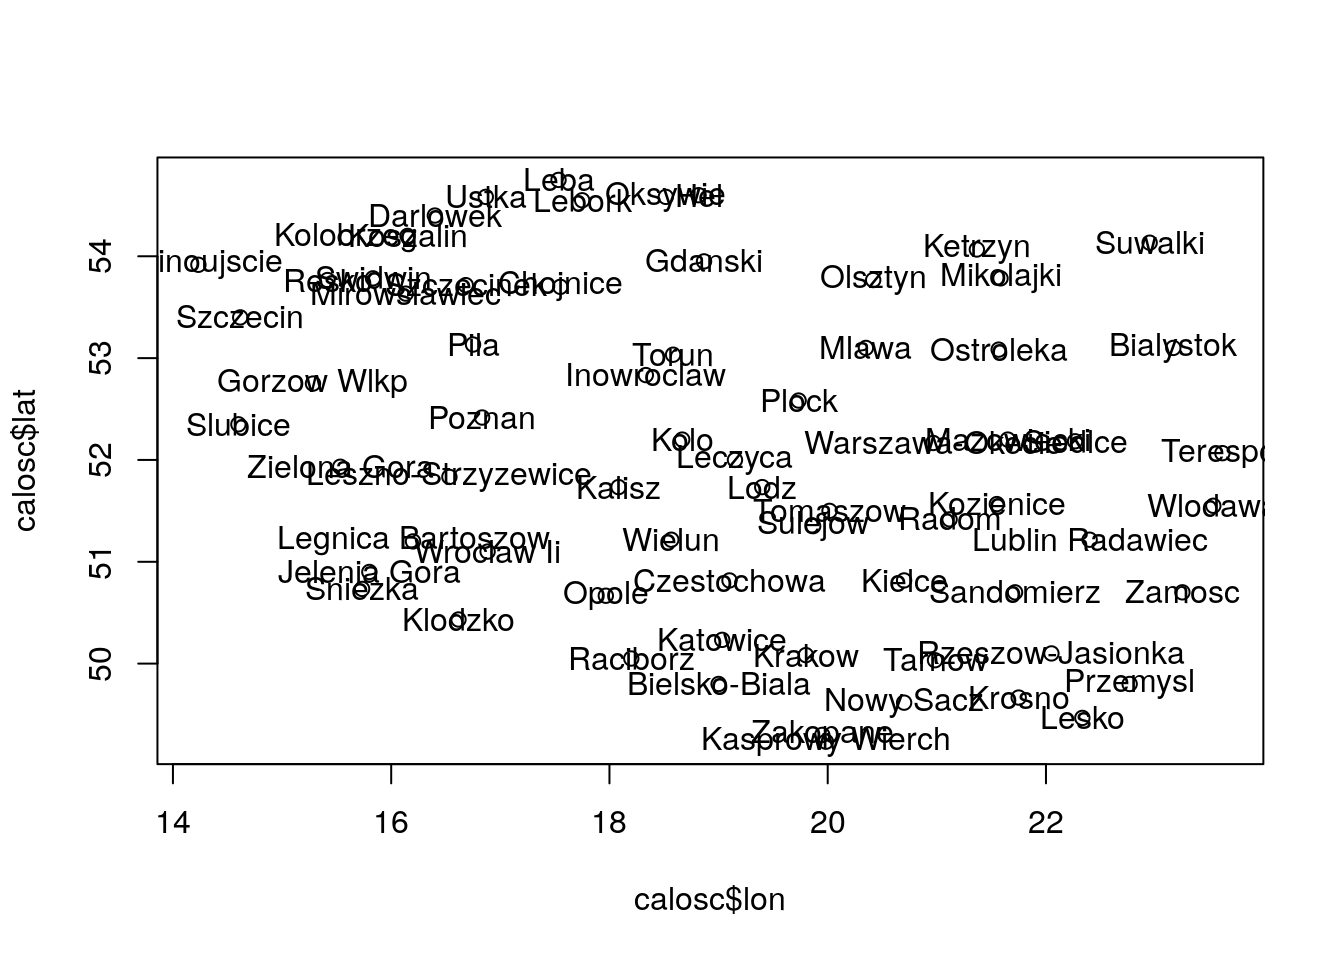
\includegraphics{ksiazka_files/figure-latex/plot_ogimet1-1} \end{center}

\begin{itemize}
\tightlist
\item
  Można dodatkowo dodać fragment kodu, który doda kontury krajów. Jeśli
  nie mamy nigdzie w pobliżu odpowiednio przygotowanej warstwy w postaci
  pliku GISowego, możemy wykorzystać pakiet \texttt{mapdata}, w którym
  znajdują się podstawowe dane z granicami administracyjnymi dla całego
  świata:
\end{itemize}

\begin{Shaded}
\begin{Highlighting}[]
\CommentTok{#install.packages("mapdata") # jesli chcemy uzyc po raz pierwszy musimy ja zainstalowac}
\KeywordTok{library}\NormalTok{(mapdata) }\CommentTok{# aktywacja pakietu}
\KeywordTok{plot}\NormalTok{(}\DataTypeTok{x =}\NormalTok{ calosc}\OperatorTok{$}\NormalTok{lon, }\DataTypeTok{y =}\NormalTok{ calosc}\OperatorTok{$}\NormalTok{lat)}
\KeywordTok{text}\NormalTok{(}\DataTypeTok{x =}\NormalTok{ calosc}\OperatorTok{$}\NormalTok{lon, }\DataTypeTok{y =}\NormalTok{ calosc}\OperatorTok{$}\NormalTok{lat, }\DataTypeTok{labels=}\NormalTok{calosc}\OperatorTok{$}\NormalTok{stacja) }\CommentTok{# rysujemy to co wczesniej}
\KeywordTok{map}\NormalTok{(}\StringTok{"world"}\NormalTok{, }\DataTypeTok{add=}\OtherTok{TRUE}\NormalTok{, }\DataTypeTok{lwd=}\DecValTok{2}\NormalTok{) }\CommentTok{# wazne aby ustawic opcje 'add'; reszta parametrow jak dla funkcji plot()}
\KeywordTok{text}\NormalTok{(}\DataTypeTok{x =}\NormalTok{ calosc}\OperatorTok{$}\NormalTok{lon, }\DataTypeTok{y =}\NormalTok{ calosc}\OperatorTok{$}\NormalTok{lat}\FloatTok{+0.2}\NormalTok{, }\DataTypeTok{labels=}\NormalTok{calosc}\OperatorTok{$}\NormalTok{tmin, }\DataTypeTok{col=}\StringTok{"blue"}\NormalTok{) }\CommentTok{# dodajmy jeszcze np. temp. min nieco powyzej etykiet}
\end{Highlighting}
\end{Shaded}

\begin{center}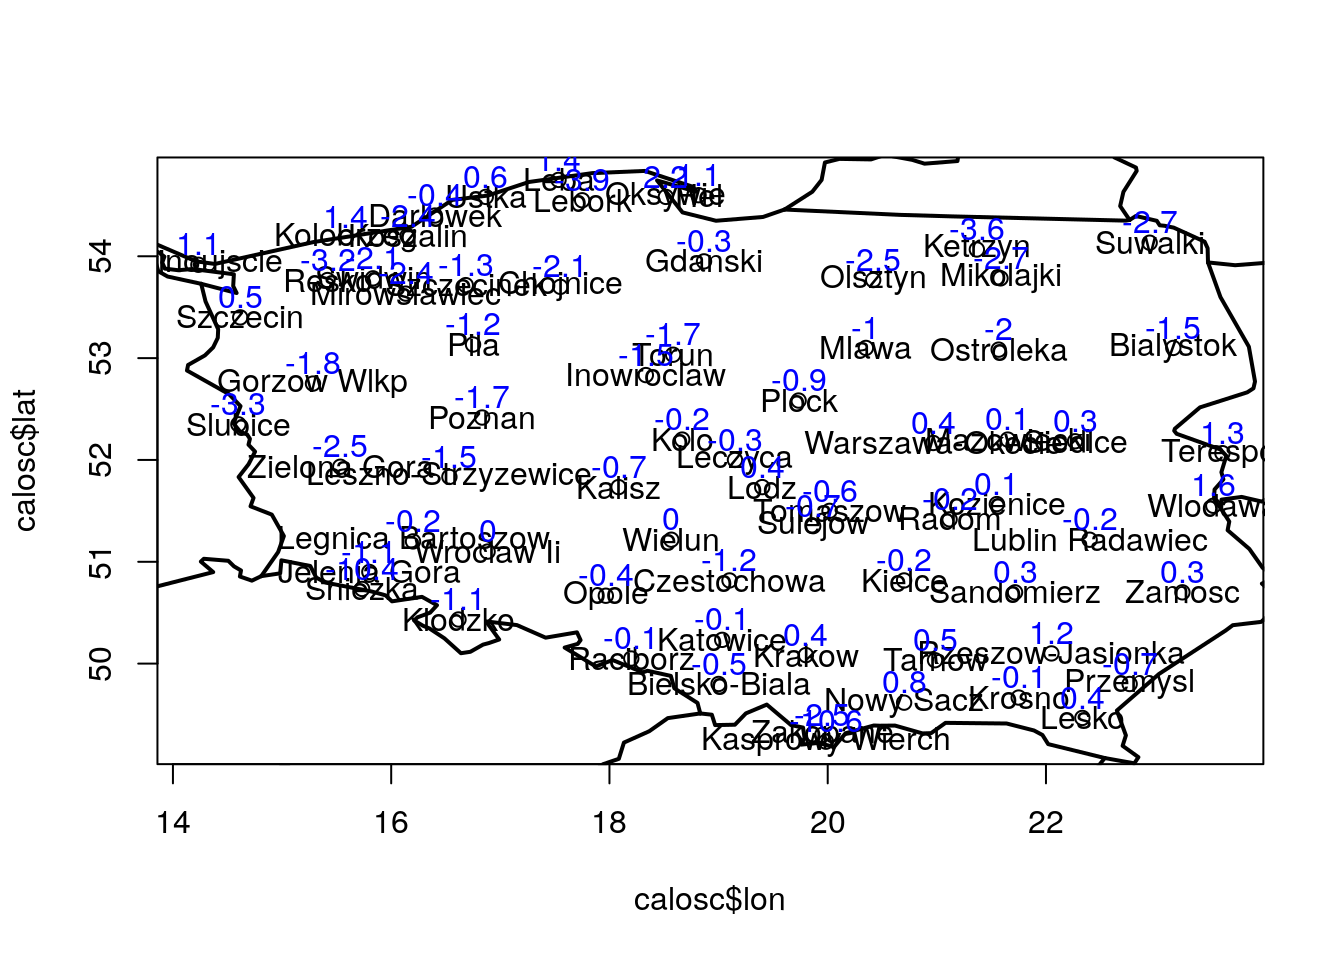
\includegraphics{ksiazka_files/figure-latex/mapdata-1} \end{center}

\subsection{Łączenie danych po dacie}\label{aczenie-danych-po-dacie}

W katalogu \url{http://enwo.pl/przetwarzanie/dane/opady/} znajdują się
pliki do dzisiejszego ćwiczenia. Zawierają one dobowe sumy opadów
atmosferycznych z kilku wybranych polskich stacji. Każdy z plików ma
taką samą strukturę zawierającą w kolejnych kolumnach: numer stacji,
nazwę stacji, datę oraz sumę opadu. Wartości są rozdzielone znakami
tabulacji, a miejsca dziesiętne są oddzielone kropkami.

\begin{verbatim}
## "V1" "V2"    "V3"    "V4"
## 249180120    "SKOCZÓW"   19501101    2.1
## 249180120    "SKOCZÓW"   19501105    2.1
## 249180120    "SKOCZÓW"   19501107    2.9
## 249180120    "SKOCZÓW"   19501108    0.5
## 249180120    "SKOCZÓW"   19501111    0.6
## 249180120    "SKOCZÓW"   19501114    12.6
## 249180120    "SKOCZÓW"   19501115    12.3
## 249180120    "SKOCZÓW"   19501116    0.6
## 249180120    "SKOCZÓW"   19501117    0.4
\end{verbatim}

Zwróć uwagę, że pliki zawierają informację jedynie o dniach, w których
wystąpiły opady na danej stacji (jeśli opadu w danym dniu nie było
wówczas jest on pominięty). Naszym celem będzie utworzenie jednolitej,
pełnej bazy, ze wszystkimi datami w zakresie występujących dat (bez
względu na to czy padało), a wartości opadów dla każdej kolejnej stacji
będą umieszczane w kolejnych kolumnach, jak na poniższym schemacie:

\begin{verbatim}
##         daty brenna chalupki cieszyn
## 1 1951-01-01     NA     12.2     7.8
## 2 1951-01-02     NA      4.8     9.6
## 3 1951-01-03    0.1      0.5     4.3
## 4 1951-01-04    0.5      0.9     7.1
## 5 1951-01-05    5.2       NA     4.0
## 6 1951-01-06   12.9       NA     3.3
\end{verbatim}

Dla wielu osób pracujących dotychczas w arkuszach kalkulacyjnych taka
postać bazy danych jest najbardziej intuicyjna w obsłudze.

Zanim przystąpisz do tworzenia bazy danych utwórz katalog \texttt{opady}
(np. na pulpicie) i zapisz do niego pliki znajdujące się pod adresem
\url{http://enwo.pl/przetwarzanie/dane/opady}. Następnie ustaw katalog
roboczy \textbf{RStudio} aby pliki były dostępne bez konieczności
wpisywania pełnej ścieżki.

W poniższej tabeli wypisano nazwy stacji oraz liczbę wierszy w każdym z
plików. \emph{Dlaczego nie możemy połączyć plików od razu do postaci
macierzy / ramki danych za pomocą komendy \texttt{cbind()} /
\texttt{cbind.data.frame()}?}

\begin{verbatim}
##    1603 BRENNA.
##    1198 CHALUPKI.
##    1198 CHAŁUPKI.
##    2053 CIESZYN.
##    1270 GOCZALKOWICE-ZDROJ.
##    1270 GOCZAŁKOWICE-ZDRÓJ.
##    1921 ISTEBNA-MLODAGORA.
##    1921 ISTEBNA-MŁODAGÓRA.
##    1947 ISTEBNA-STECOWKA.
##    1947 ISTEBNA-STECÓWKA.
##    1492 JAWISZOWICE.
##    1717 RUDZICA.
##    1763 SKOCZOW.
##    1763 SKOCZÓW.
##    1493 SZCZYRK.
##    1233 TRZEMESNIA.
##    1233 TRZEMEŚNIA.
##    1856 USTROŃ-RÓWNICA-WIEŚ.
##    1856 USTRON.
##    2032 WAPIENICA.
##    1237 WARSZOWICE.
##    1817 WISŁA-CENTRUM.
##    1268 WISLA-GLEBCE.
##    1268 WISŁA-GŁĘBCE.
##     695 WISŁAWIELKA.
##   39051
\end{verbatim}

\begin{center}\rule{0.5\linewidth}{\linethickness}\end{center}

Do połączenia 2 ramek danych na podstawie wspólnego identyfikatora można
użyć natywnie dostępnej w \textbf{R} funkcji \texttt{merge()} lub
skorzystać z pakietu \texttt{plyr}, który oferuje nieco bardziej wydajny
algorytm łączenia baz danych. W celu przetestowania jego funkcjonalności
niezbędne będzie wykonanie poniższych kroków:

\begin{enumerate}
\def\labelenumi{\arabic{enumi}.}
\tightlist
\item
  Stwórz obiekt \texttt{data} z datami od 1. stycznia 1950 r. do 31.
  grudnia 1960 r.
\item
  Stwórz ramkę danych \texttt{wynik} z jedną kolumną nazwaną
  \texttt{data}, w której będą przechowywane wartości dat (z
  poprzedniego punktu).
\item
  Wczytaj pierwszy (dowolny) plik z danymi opadowymi i nazwij go
  \texttt{dane}. Za pomocą funkcji \texttt{colnames()} nazwij w
  intuicyjny sposób kolumny (np.: ``id'',``stacja'',``data'',``opad'').
\item
  Kolumnę zawierającą datę przekonwertuj do klasy \texttt{Date}, aby
  komputer nie miał problemów ze zrozumieniem, że wartości w tej
  kolumnie przechowują czas a nie wartości liczbowe.
\item
  Złącz wynikową ramkę danych z wczytanym plikiem za pomoca funkcji
  \texttt{left\_join()} z pakietu \texttt{dplyr}.
\item
  Ponów kroki 3-5 wczytując kolejny plik do istniejącej wynikowej ramki
  danych
\end{enumerate}

\subsection*{Zadanie domowe}\label{zadanie-domowe-5}
\addcontentsline{toc}{subsection}{Zadanie domowe}

Po opanowaniu złączania ramek danych kontynuuj treść poleceń 1-6 poprzez
stworzenie pętli \texttt{for}, która będzie wczytywać kolejne pliki z
danymi opadowymi oraz dopisywać do wynikowej ramki danych. Finalny wynik
zapisz do pliku arkuszu kalkulacyjnego z rozszerzeniem \texttt{.xls}.

\chapter{dplyr - część II}\label{dplyr---czesc-ii}

W tej części zapoznawania się z możliwościami pakietu \texttt{dplyr}
dowiesz się jak w szybki sposób manipulować ramkami danych.

\emph{Ze względu na częste stosowanie rozwiazań z pakietów
\texttt{dplyr} oraz \texttt{tidyr} najbardziej popularne rozwiązania
zawarto w tzw. }cheat-sheet'ie* *
\url{https://www.rstudio.com/wp-content/uploads/2015/02/data-wrangling-cheatsheet.pdf}

\begin{center}\rule{0.5\linewidth}{\linethickness}\end{center}

\section*{Dane}\label{dane}
\addcontentsline{toc}{section}{Dane}

Przed przystąpieniem do dalszej części pracy wczytaj do środowiska
\textbf{R} godzinowe wartości pomiarów dla wybranych stacji
meteorologicznych IMGW-PIB (2000-2015). Dane do ćwiczenia przygotowano w
formacie RDS pod adresem:
\url{http://enwo.pl/przetwarzanie/dane/synop.rds}. Nazwij wczytywany
zbiór jako \texttt{dane}:

\begin{Shaded}
\begin{Highlighting}[]
\CommentTok{# Jeśli nie chcesz pobierać pliku na dysk możesz go wczytać bezpośrednio do R}
\CommentTok{# za pomocą poniższego kodu:}
\NormalTok{dane <-}\StringTok{  }\KeywordTok{readRDS}\NormalTok{(}\KeywordTok{gzcon}\NormalTok{(}\KeywordTok{url}\NormalTok{(}\StringTok{"http://enwo.pl/przetwarzanie/dane/synop.rds"}\NormalTok{)))}

\CommentTok{# ... Przyjrzyjmy się strukturze wczytanej bazy:}
\KeywordTok{head}\NormalTok{(dane)}
\end{Highlighting}
\end{Shaded}

\begin{verbatim}
##         kod nazwa   yy mm dd hh  t2m ws  wd    slp tot_cl
## 1 352160330   POZ 2000  1  1  0 -1.1  3 250 1014.2      8
## 2 352160330   POZ 2000  1  1  1 -1.1  2 280 1014.2      8
## 3 352160330   POZ 2000  1  1  2 -1.1  2 250 1014.3      8
## 4 352160330   POZ 2000  1  1  3 -1.2  2 240 1014.3      8
## 5 352160330   POZ 2000  1  1  4 -1.2  2 200 1014.3      8
## 6 352160330   POZ 2000  1  1  5 -1.0  1 170 1014.3      8
\end{verbatim}

\begin{Shaded}
\begin{Highlighting}[]
\CommentTok{# oraz:}
\KeywordTok{summary}\NormalTok{(dane)}
\end{Highlighting}
\end{Shaded}

\begin{verbatim}
##      kod               nazwa                 yy             mm        
##  Length:420766      Length:420766      Min.   :2000   Min.   : 1.000  
##  Class :character   Class :character   1st Qu.:2004   1st Qu.: 4.000  
##  Mode  :character   Mode  :character   Median :2008   Median : 7.000  
##                                        Mean   :2007   Mean   : 6.523  
##                                        3rd Qu.:2012   3rd Qu.:10.000  
##                                        Max.   :2015   Max.   :12.000  
##        dd              hh             t2m               ws        
##  Min.   : 1.00   Min.   : 0.00   Min.   :-30.10   Min.   : 0.000  
##  1st Qu.: 8.00   1st Qu.: 6.00   1st Qu.:  2.30   1st Qu.: 2.000  
##  Median :16.00   Median :12.00   Median :  9.20   Median : 3.000  
##  Mean   :15.73   Mean   :11.50   Mean   :  9.16   Mean   : 3.492  
##  3rd Qu.:23.00   3rd Qu.:17.75   3rd Qu.: 15.90   3rd Qu.: 5.000  
##  Max.   :31.00   Max.   :23.00   Max.   : 36.90   Max.   :20.000  
##        wd             slp              tot_cl     
##  Min.   :  0.0   Min.   :   0.08   Min.   :0.000  
##  1st Qu.:101.0   1st Qu.: 993.80   1st Qu.:3.000  
##  Median :200.0   Median :1000.70   Median :6.000  
##  Mean   :190.3   Mean   :1000.39   Mean   :5.191  
##  3rd Qu.:270.0   3rd Qu.:1007.20   3rd Qu.:7.000  
##  Max.   :999.0   Max.   :1038.90   Max.   :9.000
\end{verbatim}

\section{\texorpdfstring{Wybór kolumn -
\texttt{select()}}{Wybór kolumn - select()}}\label{wybor-kolumn---select}

Niejednokrotnie wczytywane przez nas zbiory danych meteorologicznych
zawierają znacznie więcej kolumn niż potrzebujemy. Jeśli chcemy wybrać
lub pozbyć się niektórych kolumn najwygodniej użyć funkcji
\texttt{select()}.

Korzystanie z funkcji \texttt{select()} wymaga podania jako pierwszego
argumentu nazwy zbioru, a następnie po przecinku (bez *" ``*) należy
podać nazwy kolumn (w dowolnej kolejności) które mają zostać
wyświetlone.

\textbf{Przykład:} Jeśli chcemy wybrać jedynie wartości z nazwą stacji,
rokiem, miesiącem, dniem, godziną, temperaturą powietrza oraz
zachmurzeniem składnia takiego polecenia wyglądała by następująco:

\begin{Shaded}
\begin{Highlighting}[]
\KeywordTok{library}\NormalTok{(dplyr) }\CommentTok{# nie zapomnijmy o aktywacji paczki dplyr po uruchomieniu RStudio!}
\NormalTok{test <-}\StringTok{ }\KeywordTok{select}\NormalTok{(dane, nazwa, yy, mm, dd, hh, t2m, tot_cl) }
\KeywordTok{head}\NormalTok{(test)}
\end{Highlighting}
\end{Shaded}

\begin{verbatim}
##   nazwa   yy mm dd hh  t2m tot_cl
## 1   POZ 2000  1  1  0 -1.1      8
## 2   POZ 2000  1  1  1 -1.1      8
## 3   POZ 2000  1  1  2 -1.1      8
## 4   POZ 2000  1  1  3 -1.2      8
## 5   POZ 2000  1  1  4 -1.2      8
## 6   POZ 2000  1  1  5 -1.0      8
\end{verbatim}

W powyższym przykładzie konieczne było podanie aż 7 z 11 nazw kolumn. W
takim przypadku można wykorzystać opcję eliminacji wybranych kolumn
poprzez zastosowanie znaku minusa ( \texttt{-} ) w odniesniu do kolumn
których chcemy się pozbyć. Taki sam efekt jak we wcześniejszym
przykładzie można uzyskać zatem poprzez:

\textbf{Przykład:}

\begin{Shaded}
\begin{Highlighting}[]
\NormalTok{test <-}\StringTok{ }\KeywordTok{select}\NormalTok{(dane, }\OperatorTok{-}\NormalTok{kod, }\OperatorTok{-}\NormalTok{ws, }\OperatorTok{-}\NormalTok{wd, }\OperatorTok{-}\NormalTok{slp)}
\KeywordTok{head}\NormalTok{(test)}
\end{Highlighting}
\end{Shaded}

\begin{verbatim}
##   nazwa   yy mm dd hh  t2m tot_cl
## 1   POZ 2000  1  1  0 -1.1      8
## 2   POZ 2000  1  1  1 -1.1      8
## 3   POZ 2000  1  1  2 -1.1      8
## 4   POZ 2000  1  1  3 -1.2      8
## 5   POZ 2000  1  1  4 -1.2      8
## 6   POZ 2000  1  1  5 -1.0      8
\end{verbatim}

Kolejne ciekawe zastosowane \texttt{select}a polega na zastosowaniu jako
operatora \texttt{:} (dwukropka), który wybierze wszystkie kolumny
znajdujące się w zakresie od wskazanej do wskazanej nazwy. Wcześniejsze
poleceni

\textbf{Przykład:}

\begin{Shaded}
\begin{Highlighting}[]
\NormalTok{test <-}\StringTok{ }\KeywordTok{select}\NormalTok{(dane, nazwa}\OperatorTok{:}\NormalTok{hh,t2m, tot_cl)}
\KeywordTok{head}\NormalTok{(test)}
\end{Highlighting}
\end{Shaded}

\begin{verbatim}
##   nazwa   yy mm dd hh  t2m tot_cl
## 1   POZ 2000  1  1  0 -1.1      8
## 2   POZ 2000  1  1  1 -1.1      8
## 3   POZ 2000  1  1  2 -1.1      8
## 4   POZ 2000  1  1  3 -1.2      8
## 5   POZ 2000  1  1  4 -1.2      8
## 6   POZ 2000  1  1  5 -1.0      8
\end{verbatim}

Więcej praktycznych przykładów zastosowania pakietu \texttt{dplyr} można
znaleźć w rzeczonym we wstępie do niniejszego rozdziału
\emph{cheat-sheetcie} w podrozdziale \emph{Helper functions for
select\ldots{} } .

\textbf{Zadanie:}

\begin{enumerate}
\def\labelenumi{\arabic{enumi}.}
\tightlist
\item
  Wybierz ze zbioru \texttt{dane} tylko kolumny dla nazwy, kodu, roku,
  miesiąca oraz zredukowanego ciśnienia atmosferycznego i zapisz je do
  zbioru \texttt{test}
\item
  Wybierz ze zbioru \texttt{dane} tylko kolumny z nazwami stacji oraz
  wszystkich parametrów meteorologicznych. Zastosuj zapis negacji (tj. z
  wykorzystaniem znaku minusa) dla usuwanych kolumn i zapisz wynik
  działania jako \texttt{test2}
\end{enumerate}

\section{Filtrowanie}\label{filtrowanie}

Duże zbiory danych meteorologicznych wymagają odfiltrowania
(usunięcia/wybrania) części informacji zapisanych w wierszach.
Odfiltrowywanie danych jest w wielu przypadkach wymagane np. w celu
znalezienia i eliminacji błędów z bazy danych lub uzyskania kształtu
ramki danych tylko dla interesujących nas przypadków.

Do wyświetlania/usuwania wybranych wierszy (oprócz poznanych wcześniej
operatorów \texttt{{[}{]}} oraz operatorów zapytań logicznych) wygodne w
użyciu może okazać się wykorzystanie funkcji \texttt{filter()}.

\textbf{Przykład 1} Baza \texttt{dane} zawiera wartości pomiarowe dla
kilku stacji meteorologicznych. Informacje o tym jakie to są stacje
można sprawdzić wyświetlając np. unikalne wartości kolumny \texttt{kod}
lub \texttt{nazwa}.

\begin{Shaded}
\begin{Highlighting}[]
\KeywordTok{unique}\NormalTok{(dane}\OperatorTok{$}\NormalTok{nazwa) }\CommentTok{# wyświetla wartości unikalne z podanego wektora}
\end{Highlighting}
\end{Shaded}

\begin{verbatim}
## [1] "POZ" "WAR" "LOD"
\end{verbatim}

Okazuje się, że w bazie są dane dla 3 stacji IMGW-PIB, które oznaczono w
bazie 3 literowymi skrótami: Poznań (POZ), Warszawa (WAR) oraz ŁÓDŹ
(LOD). Jeśli do naszej dalszej pracy potrzebna jest tylko 1 stacja (np.
Poznań), wówczas możemy odfiltrować wiersze tylko do tych zawierających
słowo ``POZ'' w kolumnie \texttt{nazwa}:

\begin{Shaded}
\begin{Highlighting}[]
\NormalTok{test <-}\StringTok{ }\KeywordTok{filter}\NormalTok{(dane, nazwa}\OperatorTok{==}\StringTok{"POZ"}\NormalTok{)}
\KeywordTok{head}\NormalTok{(test)}
\end{Highlighting}
\end{Shaded}

\begin{verbatim}
##         kod nazwa   yy mm dd hh  t2m ws  wd    slp tot_cl
## 1 352160330   POZ 2000  1  1  0 -1.1  3 250 1014.2      8
## 2 352160330   POZ 2000  1  1  1 -1.1  2 280 1014.2      8
## 3 352160330   POZ 2000  1  1  2 -1.1  2 250 1014.3      8
## 4 352160330   POZ 2000  1  1  3 -1.2  2 240 1014.3      8
## 5 352160330   POZ 2000  1  1  4 -1.2  2 200 1014.3      8
## 6 352160330   POZ 2000  1  1  5 -1.0  1 170 1014.3      8
\end{verbatim}

Zwróć uwagę, że nazwę kolumny (\texttt{nazwa}) ponownie wpisaliśmy bez
cudzysłowów, natomiast poszukiwana wartość (POZ) jest tekstem, więc tym
razem konieczne było zastosowanie \texttt{"\ "}.

\textbf{Przykład 2} Stosowane operatory logiczne dla funkcji
\texttt{filter()} są tożsame z poznanymi we wcześniejszych częściach
naszego kursu. Jeśli chcemy jednocześnie odfiltrować np. tylko wiersze,
które zawierają w kolumnie nazwa wartości ``POZ'' i jednocześnie
obejmują miesiące meteorologicznego lata (VI-VIII), to składnia takiego
polecenia może być następująca:

\begin{Shaded}
\begin{Highlighting}[]
\NormalTok{test <-}\StringTok{ }\KeywordTok{filter}\NormalTok{(dane, nazwa}\OperatorTok{==}\StringTok{"POZ"}\NormalTok{, mm}\OperatorTok{>=}\DecValTok{6} \OperatorTok{&}\StringTok{ }\NormalTok{mm}\OperatorTok{<=}\DecValTok{8}\NormalTok{)}
\KeywordTok{head}\NormalTok{(test)}
\end{Highlighting}
\end{Shaded}

\begin{verbatim}
##         kod nazwa   yy mm dd hh t2m ws  wd    slp tot_cl
## 1 352160330   POZ 2000  6  1  0 4.6  1 280 1013.2      0
## 2 352160330   POZ 2000  6  1  1 4.6  0   0 1013.6      2
## 3 352160330   POZ 2000  6  1  2 3.3  0   0 1013.7      2
## 4 352160330   POZ 2000  6  1  3 3.5  1 360 1014.0      3
## 5 352160330   POZ 2000  6  1  4 6.2  1  90 1014.3      3
## 6 352160330   POZ 2000  6  1  5 9.7  2 100 1014.6      3
\end{verbatim}

\textbf{Przykład 3} Powyższy przykład z wyborem więcej niż jednej
pasującej wartości w danej kolumnie nie zawsze musi być tak trywialny
aby dało się go rozpisać za pomocą pojedynczego wyrażenia logicznego. W
takich przypadkach można zastosować odfiltrowywanie wierszy za pomocą
porównania więcej niż jednego elementu, który musi zostać zadeklarowany
jako wektor po operatorze \texttt{\%in\%} .

Jeśli interesują nas tylko wiersze obejmujące miesiące zimowe (XII-II) i
tylko z Poznania (POZ) oraz Łodzi możemy spróbować działanie poniższej
komendy:

\begin{Shaded}
\begin{Highlighting}[]
\NormalTok{test <-}\StringTok{ }\KeywordTok{filter}\NormalTok{(dane, nazwa }\OperatorTok\StringTok{ }\KeywordTok{c}\NormalTok{(}\StringTok{"POZ"}\NormalTok{,}\StringTok{"LOD"}\NormalTok{), mm }\OperatorTok\StringTok{ }\KeywordTok{c}\NormalTok{(}\DecValTok{12}\NormalTok{,}\DecValTok{1}\NormalTok{,}\DecValTok{2}\NormalTok{))}
\KeywordTok{head}\NormalTok{(test)}
\end{Highlighting}
\end{Shaded}

\begin{verbatim}
##         kod nazwa   yy mm dd hh  t2m ws  wd    slp tot_cl
## 1 352160330   POZ 2000  1  1  0 -1.1  3 250 1014.2      8
## 2 352160330   POZ 2000  1  1  1 -1.1  2 280 1014.2      8
## 3 352160330   POZ 2000  1  1  2 -1.1  2 250 1014.3      8
## 4 352160330   POZ 2000  1  1  3 -1.2  2 240 1014.3      8
## 5 352160330   POZ 2000  1  1  4 -1.2  2 200 1014.3      8
## 6 352160330   POZ 2000  1  1  5 -1.0  1 170 1014.3      8
\end{verbatim}

\begin{Shaded}
\begin{Highlighting}[]
\KeywordTok{unique}\NormalTok{(test}\OperatorTok{$}\NormalTok{mm) }\CommentTok{# sprawdzmy czy na pewno sa tylko miesiace zimowe}
\end{Highlighting}
\end{Shaded}

\begin{verbatim}
## [1]  1  2 12
\end{verbatim}

\begin{Shaded}
\begin{Highlighting}[]
\KeywordTok{unique}\NormalTok{(test}\OperatorTok{$}\NormalTok{nazwa) }\CommentTok{# sprawdzmy czy na pewno sa tylko wybrane stacje}
\end{Highlighting}
\end{Shaded}

\begin{verbatim}
## [1] "POZ" "LOD"
\end{verbatim}

\textbf{Przykład 4} Rozpoznanie błędów w bazach danych meteorologicznych
nie należy do zadań łatwych. Część błędów można jednak dość łatwo
rozpoznać znając fizyczne ograniczenia występujących wartości. Sprawdźmy
naszą bazę pod tym kątem na przykładzie zachmurzenia ogólnego nieba,
które jest podawane w oktantach (0-8). Jeśli chcemy sprawdzić czy
istnieją wartości nie mieszczące się w tym zakresie możemy spróbować
zdefiniować takie zapytanie logiczne, które umożliwi nam zweryfikowanie
takich informacji i zapisanie ich do nowego obiektu:

\begin{Shaded}
\begin{Highlighting}[]
\NormalTok{bledy <-}\StringTok{ }\KeywordTok{filter}\NormalTok{(dane, tot_cl}\OperatorTok{<}\DecValTok{0} \OperatorTok{|}\StringTok{ }\NormalTok{tot_cl}\OperatorTok{>}\DecValTok{8}\NormalTok{)}
\KeywordTok{head}\NormalTok{(bledy)}
\end{Highlighting}
\end{Shaded}

\begin{verbatim}
##         kod nazwa   yy mm dd hh  t2m ws  wd    slp tot_cl
## 1 352160330   POZ 2000  3 23  5 -1.6  1 210 1004.5      9
## 2 352160330   POZ 2000  3 26  1  3.4  1 190 1003.1      9
## 3 352160330   POZ 2000  3 26  2  3.4  1 200 1002.9      9
## 4 352160330   POZ 2000  9  5 23  7.8  0   0 1008.6      9
## 5 352160330   POZ 2000  9  6  0  8.7  1 350 1008.6      9
## 6 352160330   POZ 2000  9  6  1  7.3  0   0 1008.6      9
\end{verbatim}

** Zadanie **

\begin{enumerate}
\def\labelenumi{\arabic{enumi}.}
\tightlist
\item
  Znajdź wiersze w których ciśnienie atmosferyczne zawiera błędne dane
\item
  Odfiltruj bazę danych w taki sposób aby zawierały tylko dane dla
  Poznania i Warszawy. Wynik zapisz do nowego obiektu \texttt{test1}
\item
  Odfiltruj bazę danych \texttt{test1} w taki sposób aby nowa baza
  \texttt{test2} zawierała tylko dane dla Poznania, z miesięcy letnich
  po roku 2005 4a. Oblicz (a) średnią, (b) minimalną i (c) maksymalną
  temperaturę powietrza jaka wystąpiła w Poznaniu w tym czasie. 4b.
  Oblicz (a) średnią (b) oraz maksymalną prędkość wiatru
\end{enumerate}

\emph{Podpowiedź: Szybkie filtrowanie danych jest dostępne również za
pomocą graficznej przeglądarki RStudio po kliknięciu w ikonę
\texttt{Filter} (ale bez możliwości zapisania wykonanego zapytania do
pliku). W trybie graficznym możliwe jest także sortowanie wierszy po
kliknięciu (jedno- lub dwukrotnym) w nazwę danej kolumny.}

\begin{figure}
\centering
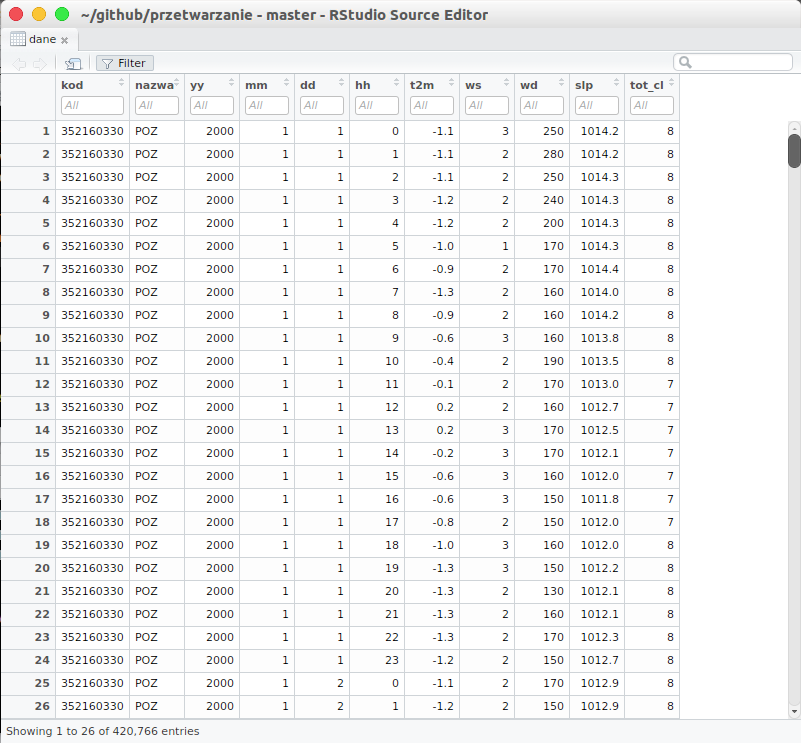
\includegraphics{figures/rstudio_filter.png}
\caption{Ekran początkowy programu \textbf{RStudio}}
\end{figure}

\section{\texorpdfstring{Sortowanie -
\texttt{arrange}}{Sortowanie - arrange}}\label{sortowanie---arrange}

Sortowanie wierszy w \textbf{R} możliwe jest na co najmniej kilka
sposobów. W pakiecie \texttt{dplyr} funkcja odpowiedzialna za sortowanie
ramek danych to \texttt{arrange()}. Działa ona bardzo podobnie do
\texttt{select()}, gdzie na pierwszym miejscu jako argument podaje się
nazwę ramki danych, a w kolejnych nazwy kolumn.

\textbf{Przykład 1} Wyświetlmy kilka najchłodniejszych pomiarów (kolumna
t2m) z całej bazy (domyślnie sortowanie odbywa się od wartości
najmniejszych do największych):

\begin{Shaded}
\begin{Highlighting}[]
\NormalTok{test <-}\StringTok{ }\KeywordTok{arrange}\NormalTok{(dane, t2m)}
\KeywordTok{head}\NormalTok{(test)}
\end{Highlighting}
\end{Shaded}

\begin{verbatim}
##         kod nazwa   yy mm dd hh   t2m ws  wd    slp tot_cl
## 1 351190465   LOD 2006  1 23  6 -30.1  0   0 1023.0      0
## 2 351190465   LOD 2006  1 23  3 -29.7  1 180 1022.0      0
## 3 351190465   LOD 2006  1 23  5 -29.7  0   0 1023.0      0
## 4 351190465   LOD 2006  1 23  2 -29.5  0   0 1022.0      0
## 5 351190465   LOD 2006  1 23  7 -29.5  0   0 1023.5      0
## 6 351190465   LOD 2006  1 22 23 -28.8  1 240 1021.0      0
\end{verbatim}

\textbf{Przykład 2} Jeśli chcemy zmienić domyślną (narastającą)
kolejność sortowania możemy odwrócić kierunek sortowania za pomocą znaku
minusa przy nazwie kolumny. Sprawdźmy zatem kilka rekordowych wartości
temperatur powietrza zanotowanych na analizowanych stacjach:

\begin{Shaded}
\begin{Highlighting}[]
\NormalTok{test <-}\StringTok{ }\KeywordTok{arrange}\NormalTok{(dane, }\OperatorTok{-}\NormalTok{t2m)}
\KeywordTok{head}\NormalTok{(test)}
\end{Highlighting}
\end{Shaded}

\begin{verbatim}
##         kod nazwa   yy mm dd hh  t2m ws  wd    slp tot_cl
## 1 351190465   LOD 2013  8  8 14 36.9  6 204  989.8      2
## 2 352160330   POZ 2015  8  8 14 36.8  1 137 1004.9      1
## 3 352200375   WAR 2013  8  8 13 36.7  4 152 1000.0      2
## 4 352200375   WAR 2013  8  8 15 36.7  2 191  999.8      4
## 5 352200375   WAR 2013  8  8 14 36.6  2 185 1000.0      4
## 6 351190465   LOD 2013  8  8 13 36.5  7 208  989.8      4
\end{verbatim}

\begin{Shaded}
\begin{Highlighting}[]
\CommentTok{# okazuje sie, ze wszedzie najcieplejszy byl 8. sierpnia, choc...}
\end{Highlighting}
\end{Shaded}

** Przykład 3 **

W przypadku w którym wartości sortowane mają takie same wartości często
wykorzystywaną procedurą jest sortowanie po większej liczbie kolumn.
Spróbujmy zatem ułożyć dane nie w kolejności dla stacji, ale po datach.
Jako że wartości dla dat przechowywane są w 4 kolumnach (od ``yy'' do
``hh'') ważne jest określenie odpowiedniej kolejności sortowania:

\begin{Shaded}
\begin{Highlighting}[]
\NormalTok{test <-}\StringTok{ }\KeywordTok{arrange}\NormalTok{(dane, yy,mm,dd,hh,nazwa)}
\KeywordTok{head}\NormalTok{(test)}
\end{Highlighting}
\end{Shaded}

\begin{verbatim}
##         kod nazwa   yy mm dd hh  t2m ws  wd    slp tot_cl
## 1 352160330   POZ 2000  1  1  0 -1.1  3 250 1014.2      8
## 2 351190465   LOD 2000  1  1  1 -1.8  2 270 1001.6      8
## 3 352160330   POZ 2000  1  1  1 -1.1  2 280 1014.2      8
## 4 352200375   WAR 2000  1  1  1  0.0  2 280 1011.2      8
## 5 351190465   LOD 2000  1  1  2 -1.7  1 250 1001.5      8
## 6 352160330   POZ 2000  1  1  2 -1.1  2 250 1014.3      8
\end{verbatim}

** Zadanie **

\begin{enumerate}
\def\labelenumi{\arabic{enumi}.}
\tightlist
\item
  Posortuj dane w kolejności od największych do najmniejszych prędkości
  wiatru. Zapisz wynik sortowania do obiektu \texttt{test}
\item
  Korzystając z komendy \texttt{table()} policz ile razy każda ze stacji
  pojawia się w zestawieniu 30-tu pomiarów z największymi prędkościami
  wiatru
\end{enumerate}

\section{Przetwarzanie potokowe}\label{przetwarzanie-potokowe}

Pakiet \texttt{dplyr} zrewolucjonizował przetwarzanie danych w
środowisku \textbf{R} na wiele sposobów. Jednym z nich jest zastosowanie
przetwarzania potokowego (zwanego również przetwarzaniem sekwencyjnym),
które nie tylko zwiększa czytelność tworzonego kodu, ale także pozwala
na pominięcie kroków pośrednich, które normalnie \emph{zapychałyby}
środowisko obliczeniowe.

W przetwarzaniu potokowym cykl przetwarzania dzieli się na odrębne
bloki, z których każdy jest połączony z następnym. Dane po przejściu
przez jeden blok trafiają do następnego, aż osiągną ostatni blok.

\begin{figure}
\centering

\includegraphics{figures/przetwarzanie_potokowe1.png}
\caption{Schemat typowego przebiegu przetwarzania potokowego przy
analizie danych}
\end{figure}

Operatorem przetwarzania potokowego w \textbf{R} jest
\texttt{\%\textgreater{}\%} , który można wygenerować w \emph{RStudio}
za pomocą skrótu klawiszowego \texttt{ctrl+shift+m}. Operator
\texttt{\%\textgreater{}\%} przekierowuje strumień informacji do
kolejnej komendy \textbf{R}, która działając na tymczasowym obiekcie
przekazuje jej wynik do kolejnego bloku obliczeń. Jeśli zaistnieje
konieczność odwołania się do informacji zawartych w strumieniu danych
można się do niego odwołać poprzez symbol \texttt{.} (kropki).

\begin{figure}
\centering

\includegraphics{figures/przetwarzanie_potokowe2.png}
\caption{Przetwarzanie potokowego w \textbf{R}}
\end{figure}

\textbf{Przykład 1} Na początek przypomnijmy sobie zawartość wbudowanego
zbioru \texttt{airquality}

\begin{Shaded}
\begin{Highlighting}[]
\KeywordTok{head}\NormalTok{(airquality)}
\end{Highlighting}
\end{Shaded}

\begin{verbatim}
##   Ozone Solar.R Wind Temp Month Day    TempC
## 1    41     190  7.4  100     5   1 37.77778
## 2    36     118  8.0   72     5   2 22.22222
## 3    12     149 12.6   74     5   3 23.33333
## 4    18     313 11.5   62     5   4 16.66667
## 5    NA      NA 14.3   56     5   5 13.33333
## 6    28      NA 14.9   66     5   6 18.88889
\end{verbatim}

Ten sam efekt możemy uzyskać stosując przetwarzanie potokowe, wiedząc,
że każda \texttt{funkcja(x)} w postaci przetwarzania potokowego to
\texttt{x\ \%\textgreater{}\%\ funkcja()}, zatem:

\begin{Shaded}
\begin{Highlighting}[]
\NormalTok{airquality }\OperatorTok\StringTok{ }\KeywordTok{head}\NormalTok{() }\CommentTok{#lub: airquality %>% head(.)}
\end{Highlighting}
\end{Shaded}

\begin{verbatim}
##   Ozone Solar.R Wind Temp Month Day    TempC
## 1    41     190  7.4  100     5   1 37.77778
## 2    36     118  8.0   72     5   2 22.22222
## 3    12     149 12.6   74     5   3 23.33333
## 4    18     313 11.5   62     5   4 16.66667
## 5    NA      NA 14.3   56     5   5 13.33333
## 6    28      NA 14.9   66     5   6 18.88889
\end{verbatim}

\textbf{Przykład 2} Jeśli chcemy wybrać jedynie dni, w których (1)
temperatura powietrza przekroczyła 90F, (2) chcemy się pozbyć
niechcianych kolumn pozostawiając jedynie kolumny
\texttt{Temp\ i\ Month\ i\ Day}, (3) chcemy posortować te dni w
kolejności od najcieplejszych do najchłodniejszych, to ten efekt przy
klasycznym przetwarzaniu danych byłby rozpisany w kilku krokach:

\begin{Shaded}
\begin{Highlighting}[]
\NormalTok{krok1 <-}\StringTok{ }\KeywordTok{filter}\NormalTok{(airquality, Temp}\OperatorTok{>}\DecValTok{90}\NormalTok{) }\CommentTok{# wybieramy wiersza w których temperatura powietrza > 90}
\NormalTok{krok2 <-}\StringTok{ }\KeywordTok{select}\NormalTok{(krok1, Temp}\OperatorTok{:}\NormalTok{Day) }\CommentTok{# wybieramy tylko wskazane kolumny}
\NormalTok{krok3 <-}\StringTok{ }\KeywordTok{arrange}\NormalTok{(krok2, }\OperatorTok{-}\NormalTok{Temp) }\CommentTok{# sortujemy od najwyższych do najniższych temperatur}
\end{Highlighting}
\end{Shaded}

Teoretycznie ten sam efekt można uzyskać w jednym kroku, stosując np.
tzw. zapis na \emph{cebulkę}, choć jego czytelność pozostawia wiele do
życzenia:

\begin{Shaded}
\begin{Highlighting}[]
  \KeywordTok{arrange}\NormalTok{(}
    \KeywordTok{select}\NormalTok{( }
      \KeywordTok{filter}\NormalTok{(airquality, Temp}\OperatorTok{>}\DecValTok{90}\NormalTok{), }\CommentTok{# pierwsza funkcja }
\NormalTok{    Temp}\OperatorTok{:}\NormalTok{Day), }\CommentTok{# dokończenie funkcji select}
 \OperatorTok{-}\NormalTok{Temp) }\CommentTok{# dokończenie funkcji arrange}
\end{Highlighting}
\end{Shaded}

\begin{verbatim}
##    Temp Month Day
## 1   100     5   1
## 2    97     8  28
## 3    96     8  30
## 4    94     8  29
## 5    94     8  31
## 6    93     6  11
## 7    93     9   3
## 8    93     9   4
## 9    92     6  12
## 10   92     7   8
## 11   92     7   9
## 12   92     8  10
## 13   92     9   2
## 14   91     7  14
## 15   91     9   1
\end{verbatim}

\textbf{Przy zastosowaniu przetwarzania potokowego:}

\begin{Shaded}
\begin{Highlighting}[]
\NormalTok{airquality }\OperatorTok\StringTok{ }\KeywordTok{filter}\NormalTok{(Temp}\OperatorTok{>}\DecValTok{90}\NormalTok{) }\OperatorTok\StringTok{ }\KeywordTok{select}\NormalTok{(Temp}\OperatorTok{:}\NormalTok{Day) }\OperatorTok\StringTok{ }\KeywordTok{arrange}\NormalTok{(}\OperatorTok{-}\NormalTok{Temp)}
\end{Highlighting}
\end{Shaded}

\begin{verbatim}
##    Temp Month Day
## 1   100     5   1
## 2    97     8  28
## 3    96     8  30
## 4    94     8  29
## 5    94     8  31
## 6    93     6  11
## 7    93     9   3
## 8    93     9   4
## 9    92     6  12
## 10   92     7   8
## 11   92     7   9
## 12   92     8  10
## 13   92     9   2
## 14   91     7  14
## 15   91     9   1
\end{verbatim}

\begin{Shaded}
\begin{Highlighting}[]
\CommentTok{# lub w wersji z kropką: airquality %>% filter(., Temp>90) %>% select(., Temp:Day) %>% arrange(., -Temp)}
\end{Highlighting}
\end{Shaded}

\textbf{Zadanie:}

\begin{enumerate}
\def\labelenumi{\arabic{enumi}.}
\tightlist
\item
  Pobierz ponownie dane z pliku
  \url{http://enwo.pl/przetwarzanie/dane/synop.rds} i zapisz jako obiekt
  \texttt{dane} (możesz także wykorzystać gotowy kod:
  \texttt{dane\ \textless{}-\ \ readRDS(gzcon(url("http://enwo.pl/przetwarzanie/dane/synop.rds")))}
  )
\item
  Korzystając z przetwarzania potokowego wybierz jedynie dane
  meteorologiczne dla Poznania
\item
  W kolejnym bloku kodu wybierz jedynie miesiące letnie (VI-VIII)
\item
  W kolejnym bloku kodu uszereguj wyniki od najniższych temperatur jakie
  odnotowano latem
\item
  Zapisz rezultat działania do nowego obiektu, który nazwiesz
  \texttt{wynik}
\end{enumerate}

\section{\texorpdfstring{\texttt{group\_by()} oraz
\texttt{summarise()}}{group\_by() oraz summarise()}}\label{group_by-oraz-summarise}

Z punktu widzenia przetwarzania danych w naukach atmosferycznych
niezwykle ważna jest możliwość szybkiego tworzenia tzw. agregatów, czyli
tworzenia podsumowań dla analizowanych zbiorów danych. Do tego celu
niezwykle przydatne są 2 funkcje z pakietu \texttt{dplyr}:
\texttt{group\_by()} oraz \texttt{summarise()}.

Jak sama nazwa wskazuje funkcja \texttt{group\_by()} grupuje zbiory
danych po unikalnych wartościach we wskazanych kolumnach ramki danych.
Przykładowo, jeśli wskażemy do grupowania kolumny \texttt{yy,\ mm,\ dd},
wówczas będą one grupowały poszczególne wiersze w ramce danych jak na
wskazanym poniżej przykładzie:

\begin{figure}
\centering
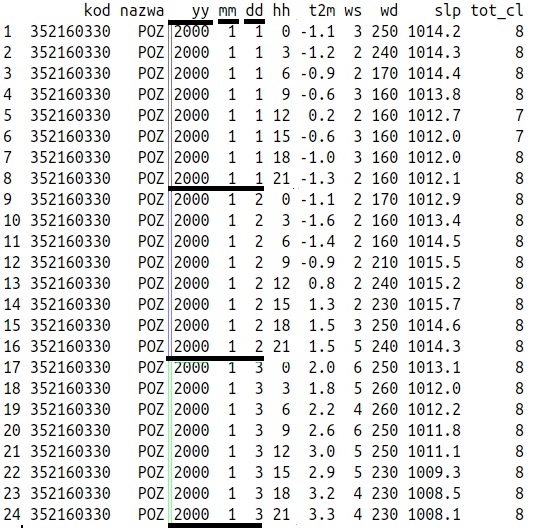
\includegraphics{figures/group_by.png}
\caption{Zasięg oddziaływania funkcji \texttt{group\_by()} przy
wskazaniu jako grupujących kolumn yy, mm, dd}
\end{figure}

Samo grupowanie nie daje widocznych efektów. Jego wynik może być jednak
z powodzeniem wykorzystany przez funkcję \texttt{summarise()}, która
pozwala na wykonanie dowolnej funkcji w obrębie wydzielonych zagregowań.
Takie postępowanie można z powodzeniem wykorzystać do obliczenia
podstawowych statystyk meteorologicznych/klimatologicznych.

\textbf{Przykład 1} Poniższy fragment kodu grupujący po kolumnie
\texttt{yy} (lata) pozwoli na zgrupowanie wszystkich wierszy, które
zawierają takie same wartości w tej kolumnie (tu: rok). Następnie dane
są przekazywane do do funkcji \texttt{summarise()}, w której obliczamy
średnie z kolumny z wartościami temperatury:

\begin{Shaded}
\begin{Highlighting}[]
\NormalTok{dane }\OperatorTok\StringTok{ }\KeywordTok{group_by}\NormalTok{(yy) }\OperatorTok\StringTok{ }\KeywordTok{summarise}\NormalTok{( }\KeywordTok{mean}\NormalTok{(t2m)  )}
\end{Highlighting}
\end{Shaded}

\begin{verbatim}
## # A tibble: 16 x 2
##       yy `mean(t2m)`
##    <int>       <dbl>
##  1  2000        9.76
##  2  2001        8.47
##  3  2002        9.38
##  4  2003        8.61
##  5  2004        8.66
##  6  2005        8.80
##  7  2006        9.20
##  8  2007        9.71
##  9  2008        9.85
## 10  2009        8.92
## 11  2010        7.77
## 12  2011        9.30
## 13  2012        8.96
## 14  2013        8.87
## 15  2014       10.1 
## 16  2015       10.2
\end{verbatim}

Czy uzyskany zbiór danych zawiera informacje dla temperatury średniej
rocznej w Poznaniu? \textbf{Nie!} W ramce danych mamy pomiary z kilku
stacji meteorologicznych. Z tego względu bez względu czy pomiar był w
Poznaniu czy Łodzi, czy w Warszawie wszystkie pomiary z danego roku
zostały wrzucone do tej samej grupy (agregaty). W takim przypadku
konieczne jest albo wcześniejsze odfiltrowania zbioru danych, albo
rozszerzenie argumentów funkcji \texttt{group\_by()}, tak aby wykonała
obliczenia dla większej liczby stacji, np.:

\begin{Shaded}
\begin{Highlighting}[]
\NormalTok{dane }\OperatorTok\StringTok{ }\KeywordTok{group_by}\NormalTok{(nazwa, yy) }\OperatorTok\StringTok{ }\KeywordTok{summarise}\NormalTok{( }\KeywordTok{mean}\NormalTok{(t2m)  )}
\end{Highlighting}
\end{Shaded}

\begin{verbatim}
## # A tibble: 48 x 3
## # Groups:   nazwa [?]
##    nazwa    yy `mean(t2m)`
##    <chr> <int>       <dbl>
##  1 LOD    2000        9.60
##  2 LOD    2001        8.13
##  3 LOD    2002        9.10
##  4 LOD    2003        8.53
##  5 LOD    2004        8.53
##  6 LOD    2005        8.64
##  7 LOD    2006        8.87
##  8 LOD    2007        9.35
##  9 LOD    2008        9.58
## 10 LOD    2009        8.63
## # ... with 38 more rows
\end{verbatim}

\textbf{Zadanie:}

\begin{enumerate}
\def\labelenumi{\arabic{enumi}.}
\tightlist
\item
  Oblicz średnie miesięczne temperatury powietrza w wieloleciu 2000-2015
  w Poznaniu (czyli np. I:-0.2*C, II:-2.1, III:+2.6, itd.)
\item
  Oblicz maksymalne temperatury jakie wystąpiły w każdym z miesięcy w
  wieloleciu 2000-2015 w Poznaniu (czyli np. 2000-I: +2.8*C,
  2000-II:+6.1, 2000-III:+12.6, itd.)
\item
  Oblicz sumę temperatur w każdym dniu kalendarzowym w Poznaniu
  (analogiczną procedurę można by było zastosować np. do opadów
  atmosferycznych)
\end{enumerate}

\emph{Wskazówka:} Nazwy kolumn w funkcji \texttt{summarise()} można
dowolnie definiować. Przykładowo, jeśli chcielibyśmy obliczyć
jednocześnie temperaturę maksymalną i minimalną dobową w Poznaniu latem
2015 r., wówczas kolumny wynikowe możemy odpowiednio nazwać: `

\begin{Shaded}
\begin{Highlighting}[]
\NormalTok{dane }\OperatorTok\StringTok{ }\KeywordTok{filter}\NormalTok{(., nazwa}\OperatorTok{==}\StringTok{"POZ"}\NormalTok{, yy}\OperatorTok{==}\DecValTok{2015}\NormalTok{, mm }\OperatorTok\StringTok{ }\KeywordTok{c}\NormalTok{(}\DecValTok{6}\OperatorTok{:}\DecValTok{8}\NormalTok{)) }\OperatorTok\StringTok{  }\KeywordTok{group_by}\NormalTok{(yy,mm,dd) }\OperatorTok\StringTok{ }\KeywordTok{summarise}\NormalTok{( }\DataTypeTok{temp_min=}\KeywordTok{min}\NormalTok{(t2m, }\DataTypeTok{na.rm=}\NormalTok{T) , }\DataTypeTok{temp_max=}\KeywordTok{max}\NormalTok{(t2m, }\DataTypeTok{na.rm=}\NormalTok{T) )}
\end{Highlighting}
\end{Shaded}

\begin{verbatim}
## # A tibble: 92 x 5
## # Groups:   yy, mm [?]
##       yy    mm    dd temp_min temp_max
##    <int> <int> <int>    <dbl>    <dbl>
##  1  2015     6     1     12.5     22.6
##  2  2015     6     2     10.7     24.9
##  3  2015     6     3     12.1     28.4
##  4  2015     6     4      9.2     21.7
##  5  2015     6     5      9.7     26.1
##  6  2015     6     6     15.2     31.6
##  7  2015     6     7     11.8     18.2
##  8  2015     6     8      9.2     20.5
##  9  2015     6     9      8.2     14.8
## 10  2015     6    10      8.6     20.7
## # ... with 82 more rows
\end{verbatim}

~

\begin{center}\rule{0.5\linewidth}{\linethickness}\end{center}

\section*{Zadanie sprawdzające}\label{zadanie-sprawdzajace-3}
\addcontentsline{toc}{section}{Zadanie sprawdzające}

\chapter{Postać wąska i szeroka}\label{postac-waska-i-szeroka}

Przechowywanie danych wiąże się nie tylko z różnymi formatami zapisu
danych, ale także z różnymi możliwościami rozłożenia tych samych
informacji na wiersze i kolumny. W analizie danych rozróżnia się dwa
podstawowe typy przechowywania informacji: postać wąską i szeroką.
\emph{``Po co taka różnorodność? Otóż w zależności od tego co z danymi
chcemy zrobić czasem lepiej je mieć w takiej czy innej postaci''}
\citep{biecek2016}

Przejście z jednej postaci do drugiej jest dość często wykonywaną
operacją (nie tylko w \textbf{R}), choć przez wielu uznawaną za operację
czasochłonną. Rozwiązaniem są funkcje pakietu \texttt{tidyr}.

\section{Postać wąska}\label{postac-waska}

Dane w postaci wąskiej mogą przypominać swoim kształtem rozwiązania
bazodanowe (np. \texttt{SQL} i pokrewne). Przykładowa baza danych
zawiera 6-godz. sumy opadów atmosferycznych pobranych ze strony
\url{https://dane.imgw.pl}. Dane dla kilku stacji zapisano do postaci
wąskiej w pliku .rds udostępnionym pod adresem:
\url{http://enwo.pl/przetwarzanie/dane/opady.rds}

\begin{enumerate}
\def\labelenumi{\arabic{enumi}.}
\tightlist
\item
  Wczytaj plik do środowiska \textbf{R} i nazwij go \texttt{dane}.
\item
  Zapoznaj się z jego strukturą za pomocą funkcji: \texttt{summary()} i
  \texttt{str()}
\item
  Sprawdź dla ilu stacji dostępne są historyczne dane opadowe?
\end{enumerate}

\begin{Shaded}
\begin{Highlighting}[]
\NormalTok{dane <-}\StringTok{  }\KeywordTok{readRDS}\NormalTok{(}\KeywordTok{gzcon}\NormalTok{(}\KeywordTok{url}\NormalTok{(}\StringTok{"http://enwo.pl/przetwarzanie/dane/opady.rds"}\NormalTok{)))}

\CommentTok{# ... Przyjrzyjmy się strukturze wczytanej bazy:}
\KeywordTok{head}\NormalTok{(dane)}
\end{Highlighting}
\end{Shaded}

\begin{verbatim}
##                  data wartosc stacja
## 1 1966-01-01 00:00:00      NA  12560
## 2 1966-01-01 06:00:00     0.4  12560
## 3 1966-01-01 12:00:00      NA  12560
## 4 1966-01-01 18:00:00     0.0  12560
## 5 1966-01-02 00:00:00     1.1  12560
## 6 1966-01-02 06:00:00      NA  12560
\end{verbatim}

\begin{Shaded}
\begin{Highlighting}[]
\CommentTok{# lub:}
\KeywordTok{str}\NormalTok{(dane)}
\end{Highlighting}
\end{Shaded}

\begin{verbatim}
## 'data.frame':    220111 obs. of  3 variables:
##  $ data   : POSIXct, format: "1966-01-01 00:00:00" "1966-01-01 06:00:00" ...
##  $ wartosc: num  NA 0.4 NA 0 1.1 NA NA NA 0.8 NA ...
##  $ stacja : num  12560 12560 12560 12560 12560 ...
\end{verbatim}

\begin{Shaded}
\begin{Highlighting}[]
\CommentTok{# Policzmy ile wartości jest dla każdej stacji}
\KeywordTok{table}\NormalTok{(dane}\OperatorTok{$}\NormalTok{stacja)}
\end{Highlighting}
\end{Shaded}

\begin{verbatim}
## 
## 12415 12520 12560 
## 74543 73655 71913
\end{verbatim}

\subsection*{\texorpdfstring{Konwersja postaci wąskiej do szerokiej -
\texttt{spread()}}{Konwersja postaci wąskiej do szerokiej - spread()}}\label{konwersja-postaci-waskiej-do-szerokiej---spread}
\addcontentsline{toc}{subsection}{Konwersja postaci wąskiej do szerokiej
- \texttt{spread()}}

Jest to typowy przykład wąskiej postaci bazy danych, który bardzo dobrze
sprawdza się np. w rozwiązaniach z grupowaniem i agregowaniem wartości
(\texttt{group\_by()} i \texttt{summarise()}). Jeśli chcielibyśmy
``przenieść'' wartości dla stacji, tak aby znajdowały się one w
kolumnach obok siebie możemy skorzystać z funkcji \texttt{spread()}.

Funkcja \texttt{spread()} wymaga zadeklarowania 3 argumentów:
\texttt{data} - zbioru danych, \texttt{key} - nazwy kolumny, która
zostanie przetransformowana jako nazwy nowych nagłówków kolumn,
\texttt{value} - nazwa kolumny z wartościami, którymi zostanie
wypełniona tabela.

Sprawdźmy działanie tej funkcji na przykładzie zbioru \texttt{dane}:

\begin{Shaded}
\begin{Highlighting}[]
\KeywordTok{library}\NormalTok{(tidyr) }\CommentTok{# musimy pakiet aktywować / instalować jeśli uruchamiany po raz pierwszy}

\KeywordTok{head}\NormalTok{(dane) }\CommentTok{# przypomnienie kształtu bazy}
\end{Highlighting}
\end{Shaded}

\begin{verbatim}
##                  data wartosc stacja
## 1 1966-01-01 00:00:00      NA  12560
## 2 1966-01-01 06:00:00     0.4  12560
## 3 1966-01-01 12:00:00      NA  12560
## 4 1966-01-01 18:00:00     0.0  12560
## 5 1966-01-02 00:00:00     1.1  12560
## 6 1966-01-02 06:00:00      NA  12560
\end{verbatim}

\begin{Shaded}
\begin{Highlighting}[]
\NormalTok{wynik <-}\StringTok{ }\KeywordTok{spread}\NormalTok{(dane, stacja, wartosc) }\CommentTok{# konwertujemy do postaci szerokiej}
\KeywordTok{head}\NormalTok{(wynik) }\CommentTok{# i sprawdzamy otrzymany wynik}
\end{Highlighting}
\end{Shaded}

\begin{verbatim}
##                  data 12415 12520 12560
## 1 1966-01-01 00:00:00   0.0    NA    NA
## 2 1966-01-01 06:00:00    NA    NA   0.4
## 3 1966-01-01 12:00:00   0.0    NA    NA
## 4 1966-01-01 18:00:00   0.9   0.0   0.0
## 5 1966-01-02 00:00:00   1.1   1.3   1.1
## 6 1966-01-02 06:00:00    NA    NA    NA
\end{verbatim}

\textbf{Zadania}

\begin{enumerate}
\def\labelenumi{\arabic{enumi}.}
\tightlist
\item
  Sprawdź co się stanie jeśli odwrócisz kolejnosć argumentów
  \texttt{key} i \texttt{value}?
\item
  Za pomocą funkcji \texttt{group\_by()} oraz \texttt{summarise()}
  oblicz roczną sumę opadów na każdej ze stacji a następnie wynik tego
  działania przekonwertuj do dowolnej postaci szerokiej
\end{enumerate}

\section{Postać szeroka}\label{postac-szeroka}

Często bardziej intuicyjna w działaniu jest postać szeroka, która
wizualnie pozwala na przeglądnięcie większej liczby danych. Czasem taki
format danych może nie być zgodny np. z niektórymi funkcjami
graficznymi, stąd konieczność transformacji z postaci szerokiej do
wąskiej.

\subsection*{\texorpdfstring{Konwersja postaci szerokiej do wąskiej -
\texttt{gather()}}{Konwersja postaci szerokiej do wąskiej - gather()}}\label{konwersja-postaci-szerokiej-do-waskiej---gather}
\addcontentsline{toc}{subsection}{Konwersja postaci szerokiej do wąskiej
- \texttt{gather()}}

Wczytaj zbiór ze średnimi miesięcznymi temperaturami powietrza w Polsce
po 1971 r.: \url{http://enwo.pl/przetwarzanie/dane/pl1.csv}. Nazwij
zbiór \texttt{pl} i zapoznaj się z jego strukturą.

\begin{Shaded}
\begin{Highlighting}[]
\NormalTok{pl <-}\StringTok{ }\KeywordTok{read.csv}\NormalTok{(}\StringTok{"http://enwo.pl/przetwarzanie/dane/pl1.csv"}\NormalTok{)}
\KeywordTok{head}\NormalTok{(pl)}
\end{Highlighting}
\end{Shaded}

\begin{verbatim}
##    rok     I    II   III   IV     V    VI   VII  VIII    IX    X   XI
## 1 1971 -2.96  0.37 -0.11 7.41 14.48 14.91 17.81 18.74 11.25 8.39 2.61
## 2 1972 -5.81  0.27  3.91 7.36 12.48 16.25 19.40 16.56 11.36 6.14 4.36
## 3 1973 -1.67  1.27  3.69 6.13 12.35 15.77 17.58 17.12 13.14 6.62 1.85
## 4 1974  0.06  2.29  4.37 6.89 10.75 14.04 15.62 17.70 13.40 6.29 3.86
## 5 1975  2.97 -0.56  3.87 6.58 13.35 15.40 18.55 18.27 15.79 7.98 1.75
## 6 1976 -1.97 -3.32 -0.85 6.72 11.95 15.09 18.06 15.31 12.58 7.59 4.71
##     XII
## 1  3.02
## 2 -0.01
## 3 -0.72
## 4  2.73
## 5  0.88
## 6 -1.24
\end{verbatim}

W przypadku funkcji \texttt{gather()} służącej do konwertowania
szerokiej postaci danych do wąskiej zestaw argumentów jest następujący:
1) \texttt{data} - ramka danych, 2) \texttt{key} oraz \texttt{value} -
etykiety nowych kolumn z kluczem i wartościami, 3) \texttt{...} -
ustalenie kolumn które mają zostać przekonwertowane według schematu dla
paczek \texttt{dplyr/tidyr} (tj. bez '', z możliwością stosowania
\texttt{:} dla kolumny początkowej i końcowej, itp.)

W naszym przypadku ramkę danych \texttt{pl} chcemy skonwertować tak, aby
zawierała 3 kolumny: \texttt{rok}, \texttt{miesiac},
\texttt{temperatura}.

\begin{Shaded}
\begin{Highlighting}[]
\NormalTok{wynik <-}\StringTok{ }\KeywordTok{gather}\NormalTok{(}\DataTypeTok{data=}\NormalTok{pl, }\DataTypeTok{key=}\StringTok{"miesiac"}\NormalTok{, }\DataTypeTok{value=}\StringTok{"temperatura"}\NormalTok{, I}\OperatorTok{:}\NormalTok{XII)}
\KeywordTok{head}\NormalTok{(wynik)}
\end{Highlighting}
\end{Shaded}

\begin{verbatim}
##    rok miesiac temperatura
## 1 1971       I       -2.96
## 2 1972       I       -5.81
## 3 1973       I       -1.67
## 4 1974       I        0.06
## 5 1975       I        2.97
## 6 1976       I       -1.97
\end{verbatim}

\section{Sklejanie i rozszczepianie
kolumn}\label{sklejanie-i-rozszczepianie-kolumn}

Ostatnie 2 ciekawe funkcje z pakietu \texttt{tidyr} to sklejanie (
\texttt{unite()} ) i rozszczepianie kolumn ( \texttt{seperate()} ). Ze
względu na ograniczenia czasowe polecam zapoznanie się z tymi funkcjami
indywidualnie

\begin{center}\rule{0.5\linewidth}{\linethickness}\end{center}

\emph{Pamiętaj o cheat-sheet'ie łączącym najważniejsze funkcje pakietów:
dplyr i tidyr}
\url{https://www.rstudio.com/wp-content/uploads/2015/02/data-wrangling-cheatsheet.pdf}

\chapter{Grafika}\label{grafika}

Wstępne przetwarzanie danych jest tylko jednym z etapów pracy z danymi.
Finalnym produktem przetwarzania są bardzo często wizualizacje tych
danych w postaci graficznej. W przypadku \textbf{R} istnieje kilka
silników graficznych, spośród których najbardziej popularny jest bazowy
\texttt{graphics} oraz pakiet \texttt{ggplot2} i \texttt{lattice}.

Poniżej wymieniono

\section{graphics}\label{graphics}

Podstawowy silnik graficzny \textbf{R}.

Funkcje:

\begin{itemize}
\tightlist
\item
  \texttt{plot()} + \texttt{lines()}
\end{itemize}

\begin{Shaded}
\begin{Highlighting}[]
\NormalTok{dane <-}\StringTok{  }\KeywordTok{readRDS}\NormalTok{(}\KeywordTok{gzcon}\NormalTok{(}\KeywordTok{url}\NormalTok{(}\StringTok{"http://enwo.pl/przetwarzanie/dane/opady.rds"}\NormalTok{)))}
\NormalTok{dane <-}\StringTok{ }\NormalTok{dane }\OperatorTok\StringTok{ }\KeywordTok{group_by}\NormalTok{(}\DataTypeTok{rok=}\NormalTok{lubridate}\OperatorTok{::}\KeywordTok{year}\NormalTok{(dane}\OperatorTok{$}\NormalTok{data), stacja)  }\OperatorTok\StringTok{ }\KeywordTok{summarise}\NormalTok{( }\DataTypeTok{suma=}\KeywordTok{sum}\NormalTok{(wartosc, }\DataTypeTok{na.rm =}\NormalTok{ T)) }
\NormalTok{dane <-}\StringTok{ }\KeywordTok{filter}\NormalTok{(dane, rok}\OperatorTok{<}\DecValTok{2017}\NormalTok{) }\CommentTok{# ostatni rok jest niepelny}
\NormalTok{dane2 <-}\StringTok{ }\KeywordTok{filter}\NormalTok{(dane,stacja}\OperatorTok{==}\StringTok{"12415"}\NormalTok{)}
\end{Highlighting}
\end{Shaded}

\begin{Shaded}
\begin{Highlighting}[]
\KeywordTok{plot}\NormalTok{(}\DataTypeTok{x =}\NormalTok{ dane2}\OperatorTok{$}\NormalTok{rok, }\DataTypeTok{y =}\NormalTok{ dane2}\OperatorTok{$}\NormalTok{suma, }\DataTypeTok{type=}\StringTok{'l'}\NormalTok{, }\DataTypeTok{main=}\StringTok{"tytuł"}\NormalTok{, }\DataTypeTok{xlab=}\StringTok{'rok'}\NormalTok{, }\DataTypeTok{ylab=}\StringTok{'suma [mm]'}\NormalTok{, }\DataTypeTok{lwd=}\DecValTok{2}\NormalTok{)}
\end{Highlighting}
\end{Shaded}

\begin{verbatim}
## Warning in title(...): conversion failure on 'tytuł' in 'mbcsToSbcs': dot
## substituted for <c5>
\end{verbatim}

\begin{verbatim}
## Warning in title(...): conversion failure on 'tytuł' in 'mbcsToSbcs': dot
## substituted for <82>
\end{verbatim}

\begin{Shaded}
\begin{Highlighting}[]
\KeywordTok{lines}\NormalTok{(}\DataTypeTok{x =}\NormalTok{ dane2}\OperatorTok{$}\NormalTok{rok, }\DataTypeTok{y =} \KeywordTok{jitter}\NormalTok{(dane2}\OperatorTok{$}\NormalTok{suma,}\DecValTok{3000}\NormalTok{), }\DataTypeTok{type=}\StringTok{'l'}\NormalTok{, }\DataTypeTok{col=}\StringTok{"red"}\NormalTok{, }\DataTypeTok{lty=}\DecValTok{2}\NormalTok{, }\DataTypeTok{lwd=}\DecValTok{2}\NormalTok{)}
\end{Highlighting}
\end{Shaded}

\begin{figure}

{\centering 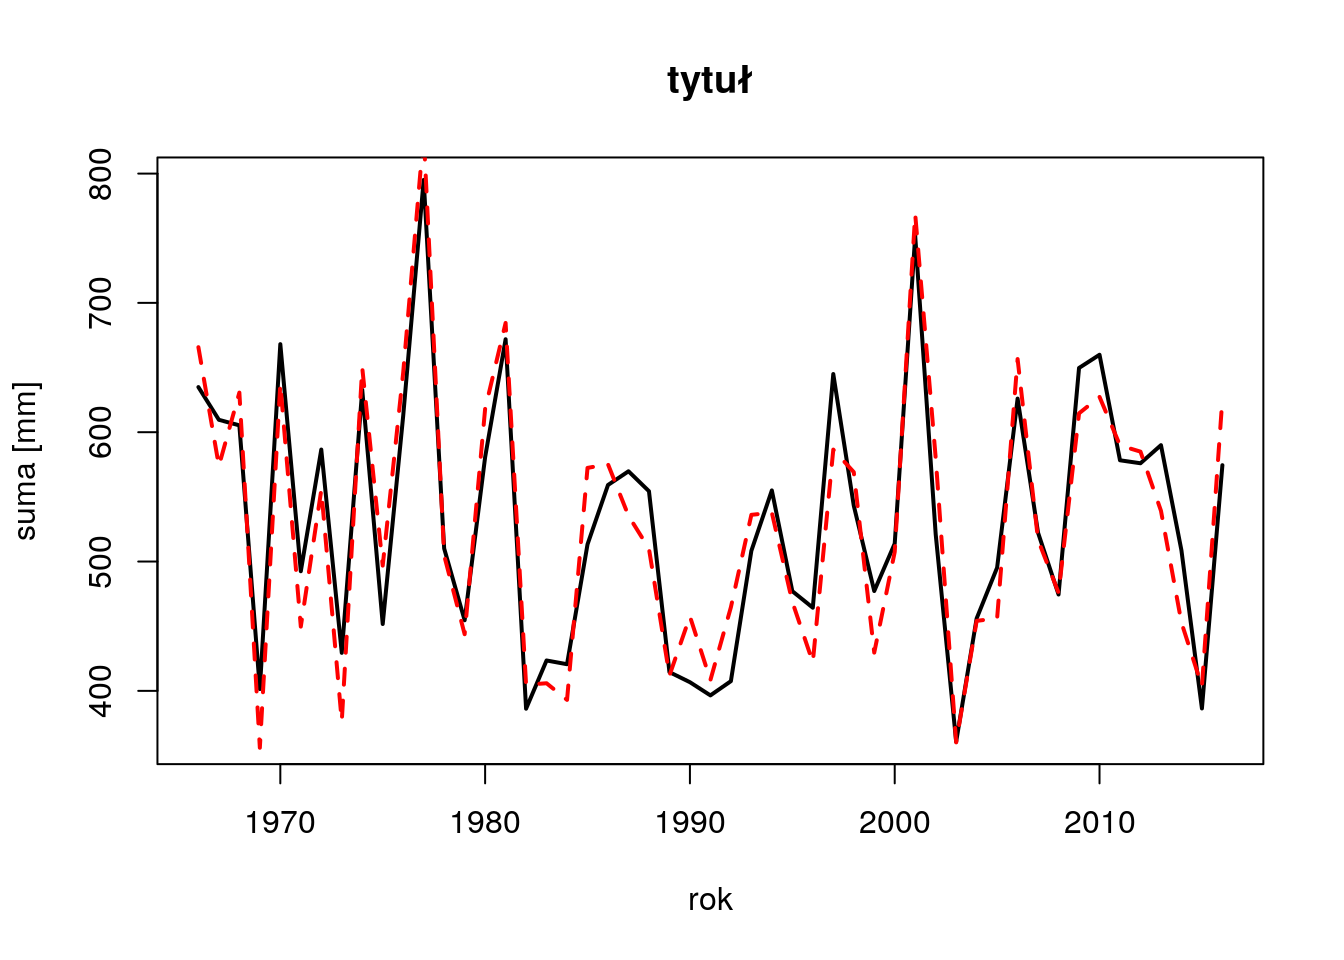
\includegraphics[width=0.8\linewidth]{ksiazka_files/figure-latex/unnamed-chunk-6-1} 

}

\caption{Przykład użycia funkcji plot i lines}\label{fig:unnamed-chunk-6}
\end{figure}

\begin{itemize}
\tightlist
\item
  \texttt{boxplot()}
\end{itemize}

\begin{Shaded}
\begin{Highlighting}[]
\NormalTok{tidyr}\OperatorTok{::}\KeywordTok{spread}\NormalTok{(dane, rok, suma) }\OperatorTok\StringTok{ }\NormalTok{.[,}\OperatorTok{-}\DecValTok{1}\NormalTok{] }\OperatorTok\StringTok{ }\KeywordTok{boxplot}\NormalTok{()}
\end{Highlighting}
\end{Shaded}

\begin{figure}

{\centering 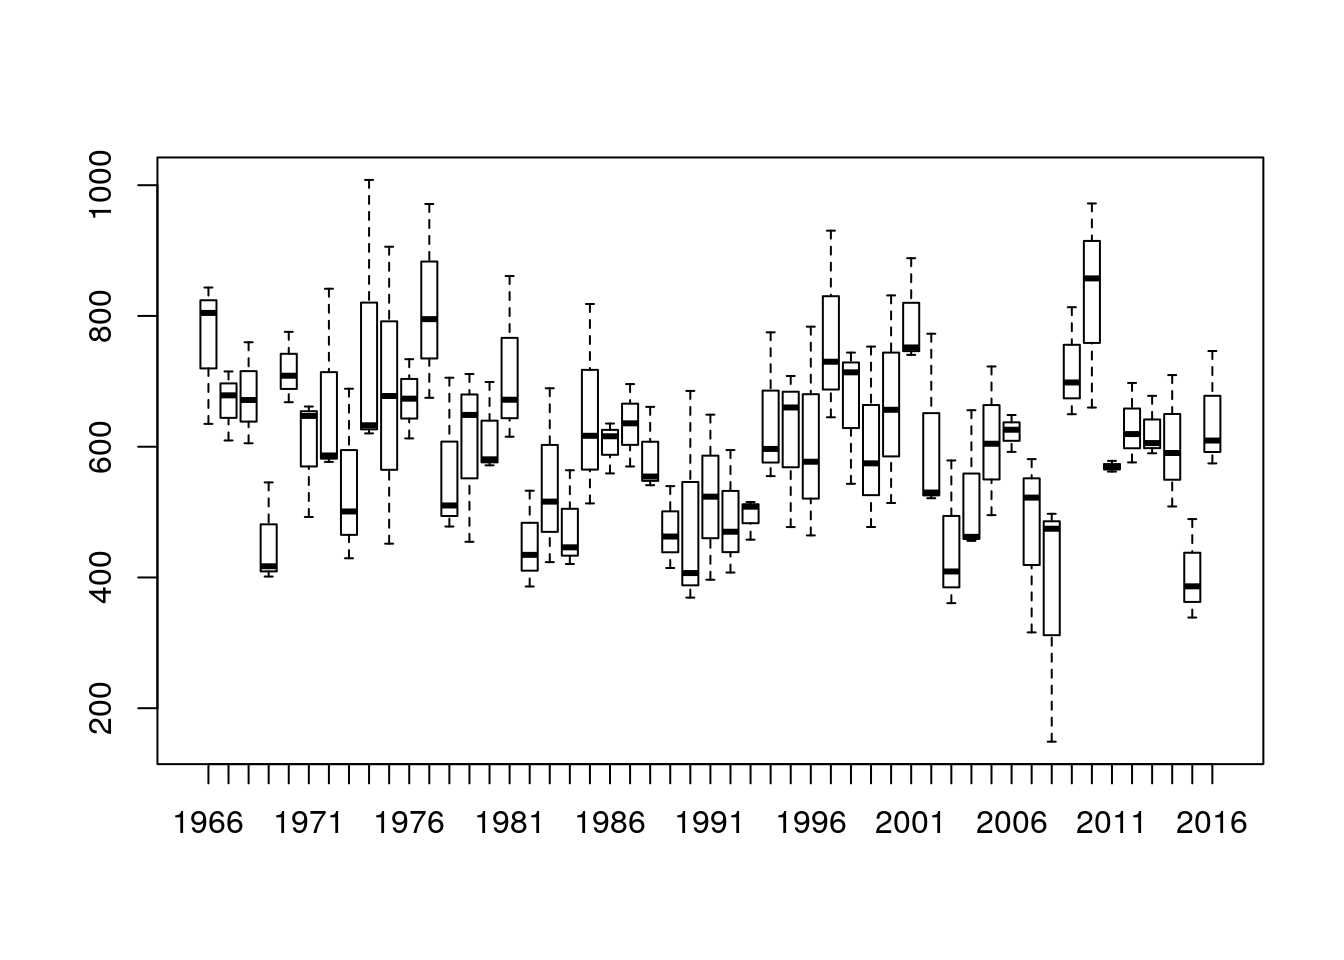
\includegraphics[width=0.8\linewidth]{ksiazka_files/figure-latex/unnamed-chunk-7-1} 

}

\caption{Przykład użycia funkcji boxplot dla sumy opadów atmosferycznych na kilku stacjach}\label{fig:unnamed-chunk-7}
\end{figure}

\begin{itemize}
\tightlist
\item
  \texttt{barplot()}
\end{itemize}

\begin{Shaded}
\begin{Highlighting}[]
\NormalTok{tidyr}\OperatorTok{::}\KeywordTok{spread}\NormalTok{(dane2, rok, suma) }\OperatorTok\StringTok{ }\KeywordTok{as.numeric}\NormalTok{() }\OperatorTok\StringTok{ }\NormalTok{.[}\OperatorTok{-}\DecValTok{1}\NormalTok{] }\OperatorTok\StringTok{ }\KeywordTok{barplot}\NormalTok{(., }\DataTypeTok{col=}\StringTok{"lightblue"}\NormalTok{)}
\end{Highlighting}
\end{Shaded}

\begin{figure}
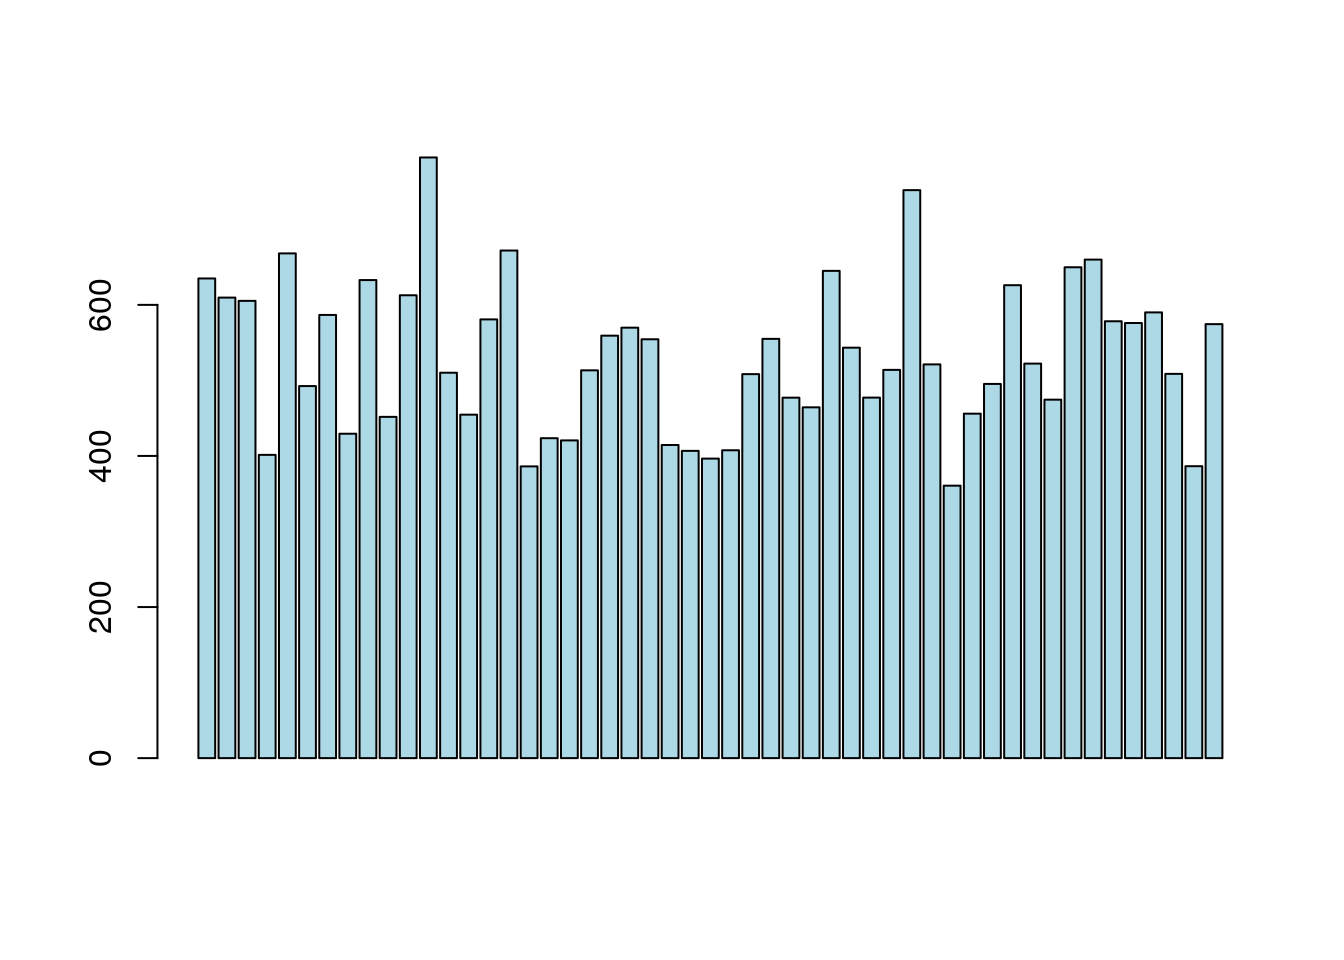
\includegraphics[width=0.8\linewidth]{ksiazka_files/figure-latex/unnamed-chunk-8-1} \caption{Przykład użycia funkcji barplot dla sumy opadów atmosferycznych}\label{fig:unnamed-chunk-8}
\end{figure}

\begin{itemize}
\tightlist
\item
  \texttt{image()}
\item
  \texttt{persp()}
\item
  \texttt{wireframe()}
\end{itemize}

\section{ggplot2}\label{ggplot2}

Grammar of graphics: \url{https://github.com/tidyverse/ggplot2/wiki}

Składnia zdecydowanie trudniejsza niż bazowego interfejsu graphics,
jednak dająca w bardziej skrótowej postaci większe możliwości:

\begin{Shaded}
\begin{Highlighting}[]
\KeywordTok{library}\NormalTok{(ggplot2)}
\KeywordTok{ggplot}\NormalTok{(dane) }\CommentTok{#nic sie nie dzieje}
\end{Highlighting}
\end{Shaded}


\includegraphics{ksiazka_files/figure-latex/ggplot2-example1-1.pdf}

\begin{Shaded}
\begin{Highlighting}[]
\KeywordTok{ggplot}\NormalTok{(dane)}\OperatorTok{+}\KeywordTok{geom_point}\NormalTok{(}\KeywordTok{aes}\NormalTok{(rok,suma))}\OperatorTok{+}\KeywordTok{facet_wrap}\NormalTok{(}\OperatorTok{~}\NormalTok{stacja)}
\end{Highlighting}
\end{Shaded}

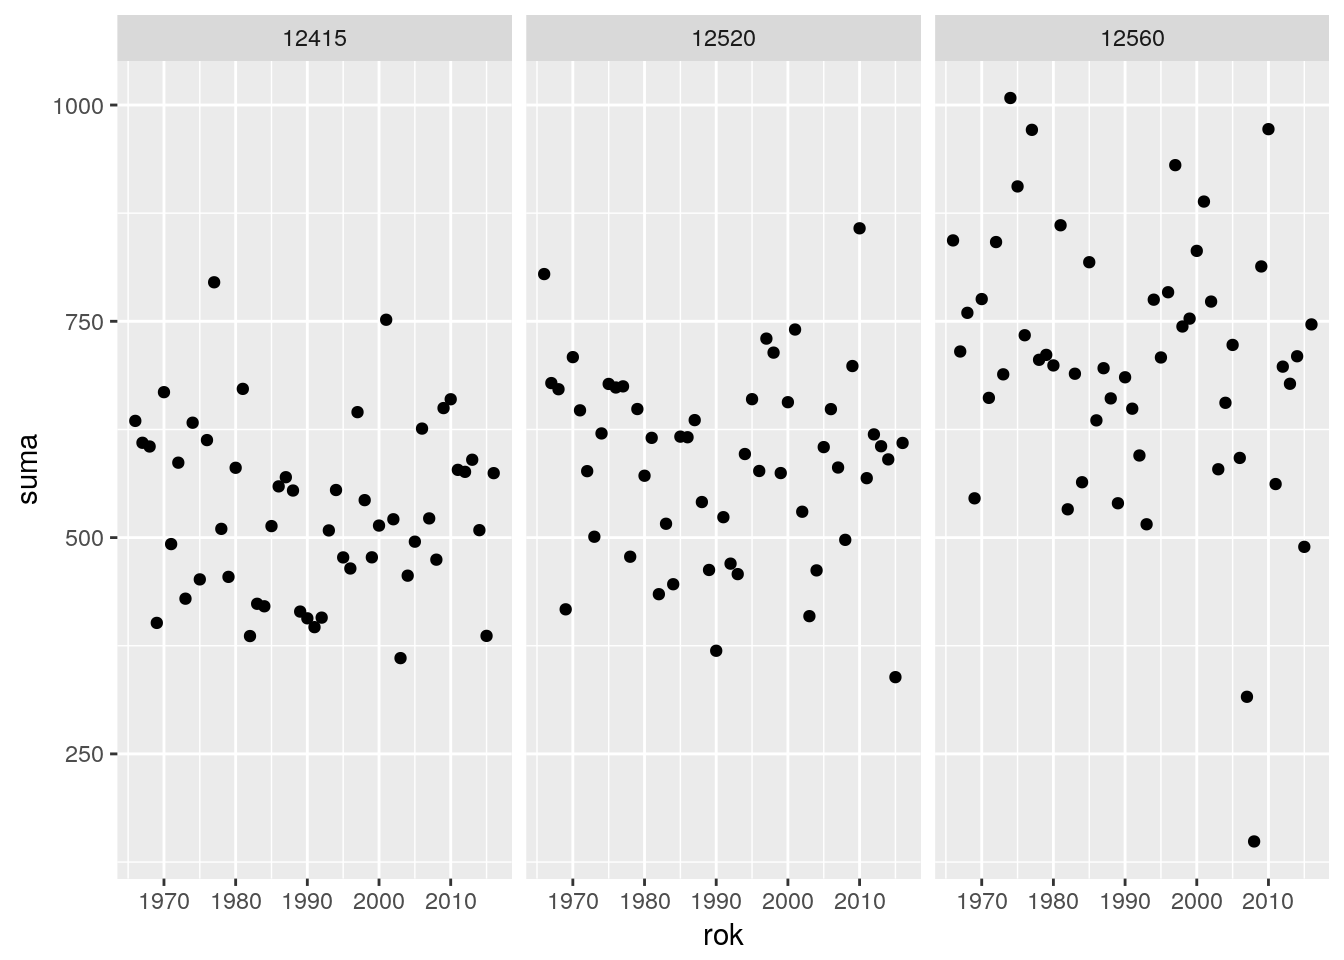
\includegraphics{ksiazka_files/figure-latex/ggplot2-example1-2.pdf}

\begin{Shaded}
\begin{Highlighting}[]
\KeywordTok{ggplot}\NormalTok{(dane)}\OperatorTok{+}\KeywordTok{geom_line}\NormalTok{(}\KeywordTok{aes}\NormalTok{(rok,suma))}\OperatorTok{+}\KeywordTok{facet_wrap}\NormalTok{(}\OperatorTok{~}\NormalTok{stacja)}
\end{Highlighting}
\end{Shaded}

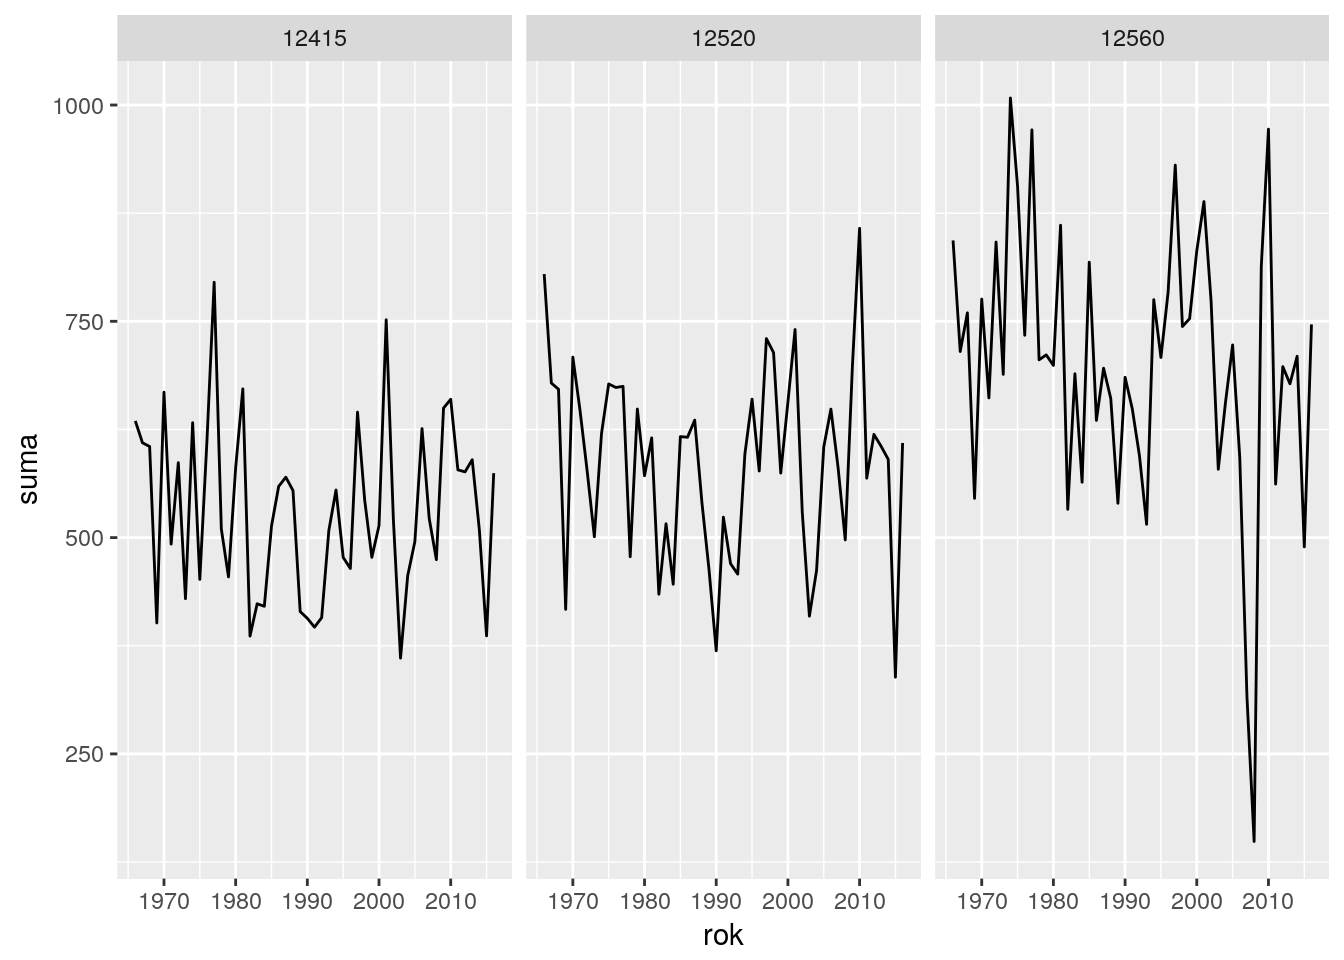
\includegraphics{ksiazka_files/figure-latex/ggplot2-example1-3.pdf}

\begin{Shaded}
\begin{Highlighting}[]
\KeywordTok{ggplot}\NormalTok{(dane)}\OperatorTok{+}\KeywordTok{geom_smooth}\NormalTok{(}\KeywordTok{aes}\NormalTok{(rok,suma),}\DataTypeTok{stat=}\StringTok{"smooth"}\NormalTok{)}\OperatorTok{+}\KeywordTok{facet_wrap}\NormalTok{(}\OperatorTok{~}\NormalTok{stacja)}
\end{Highlighting}
\end{Shaded}

\begin{verbatim}
## `geom_smooth()` using method = 'loess'
\end{verbatim}

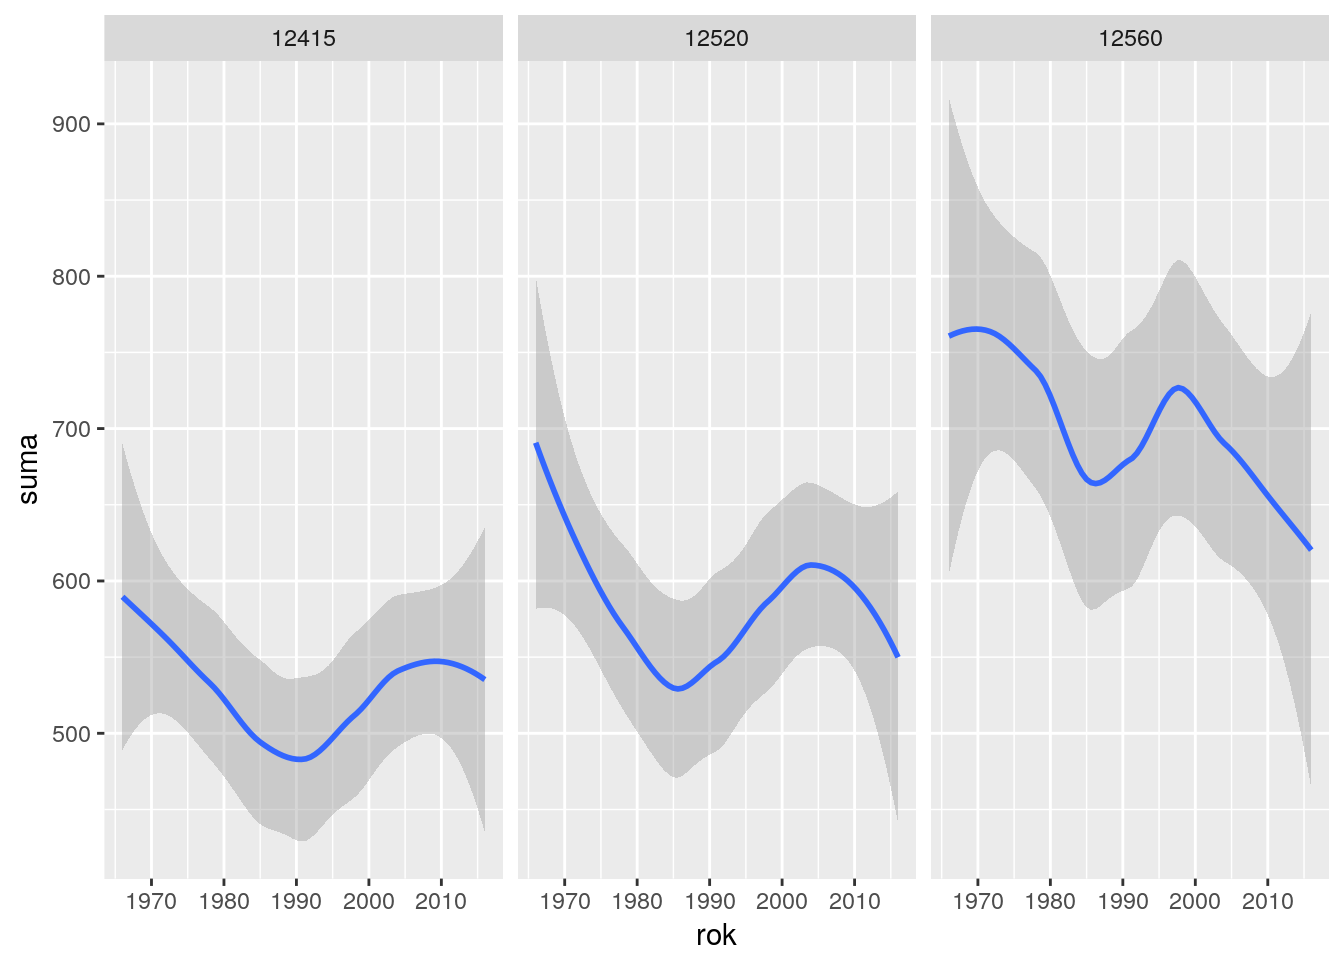
\includegraphics{ksiazka_files/figure-latex/ggplot2-example1-4.pdf}

tutorial wprowadzający do ggplot2:
\url{http://r-statistics.co/Complete-Ggplot2-Tutorial-Part1-With-R-Code.html}

przykłady dobrych wykresów wraz z kodem do ggplot2:
\url{http://r-statistics.co/Top50-Ggplot2-Visualizations-MasterList-R-Code.html}

\chapter*{Instalacja}\label{instalacja}
\addcontentsline{toc}{chapter}{Instalacja}

Najczęściej spotykana konfiguracja środowiska pracy z \textbf{R} wymaga
zainstalowania 2 programów: \textbf{R} oraz \textbf{RStudio}. Ważne, aby
były one instalowane w odpowiedniej kolejności (tj. 1. \textbf{R}, 2.
\textbf{RStudio})

\section*{\texorpdfstring{Instalacja
\textbf{R}}{Instalacja R}}\label{instalacja-r}
\addcontentsline{toc}{section}{Instalacja \textbf{R}}

\textbf{R} jest dostępny praktycznie dla każdego współczesnego systemu
operacyjnego. Pliki źródłowe \textbf{R} są udostępniane na stronie
internetowej CRAN (The Comprehensive R Archive Network) pod adresem
\url{http://cran.r-project.org/}.

W przypadku większości komputerów stacjonarnych należy wybrać 64-bitową
opcję instalacji i dalej postępować zgodnie ze wskazówkami instalatora.

Po uruchomieniu programu okno pracy powinno wyglądać w środowisku
Windows jak na poniższym obrazie:

\begin{figure}
\centering
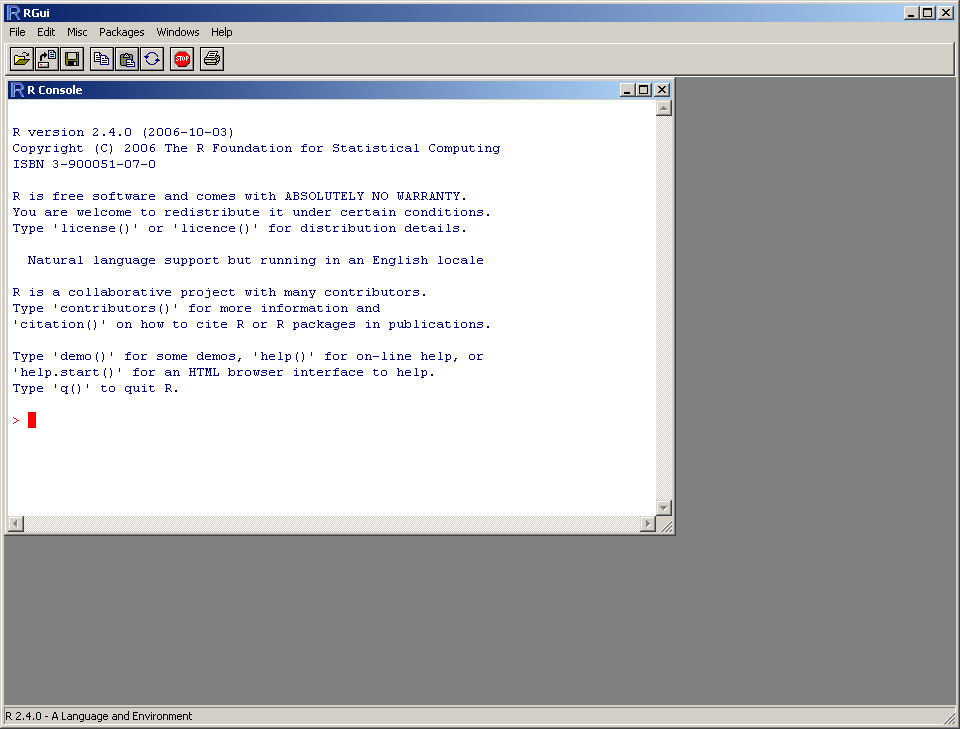
\includegraphics{figures/r_windows.png}
\caption{Ekran początkowy programu \textbf{R} w Windowsie}
\end{figure}

\textbf{Linux:}

\begin{quote}
Dla systemów operacyjnych Linux zdecydowanie wygodniej wykorzystać
wewnętrzne narzędzie instalacyjne. Przykładowo, dla systemu
Debian/Ubuntu środowisko programistyczne \textbf{R} można zainstalować
wpisując w terminalu komendę \emph{sudo apt-get install r-base}
\end{quote}

\section*{\texorpdfstring{Instalacja
\textbf{RStudio}}{Instalacja RStudio}}\label{instalacja-rstudio}
\addcontentsline{toc}{section}{Instalacja \textbf{RStudio}}

\textbf{RStudio}

Praca z \textbf{R} jest zdecydowanie bardziej przyjemna przy użyciu
zintegrowanego środowiska programistycznego (IDE, ang. \emph{Integrated
Development Environment}) \textbf{RStudio}. Program ten jest swojego
rodzaju nakładką graficzną na ``surowy \textbf{R}'' i można go pobrać ze
strony \url{http://www.rstudio.com/products/rstudio/download/}. Po
wejściu na stronę należy wybrać bezpłatną wersję programu (RStudio
Desktop) odpowiednią dla naszego systemu operacyjnego z listy
\emph{``Installers for Supported Platforms''}. Po pobraniu wskazanego
pliku instalator przeprowadzi nas przez intuicyjny proces instalacji.
Przy pierwszym uruchomieniu program \textbf{RStudio} powinien wyglądać
jak na zrzucie ekranu poniżej:

\begin{figure}
\centering
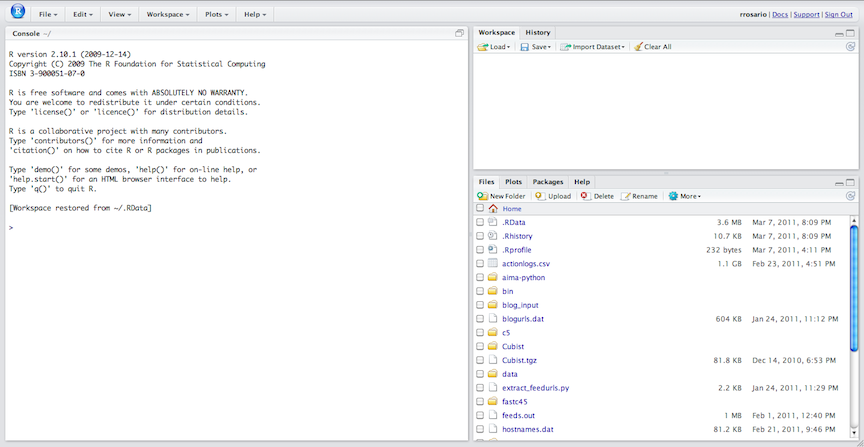
\includegraphics{figures/rstudio.png}
\caption{Ekran początkowy programu \textbf{RStudio}}
\end{figure}

\begin{quote}
\textbf{RStudio} dostarczane jest w wielu różnych wersjach, w tym także
w bezpłatnej wersji \textbf{RStudio Server} umożliwiającej pracę zdalną
z poziomu przeglądarki internetowej. Pozostałe wersje o szerszym
wachlarzu zaawansowanych opcji programistycznych są udostępniane
odpłatnie.
\end{quote}

\section*{Instalacja bibliotek}\label{instalacja-bibliotek}
\addcontentsline{toc}{section}{Instalacja bibliotek}

\textbf{R} posiada ogromną liczbę bibliotek programistycznych
rozszerzających jego możliwości. W niniejszym podręczniku będziemy
korzystać przynajmniej z kilku takich pakietów, które przed
uruchomieniem muszą zostać zainstalowane za pomocą funkcji
\texttt{install.packages()}. Przykładowo, jeśli chcesz zainstalować
bibliotekę \texttt{dplyr} i masz dostęp do internetu wystarczy użyć
komendy
\texttt{install.packages(\textquotesingle{}dplyr\textquotesingle{})}.
Bibliotekę instaluje się tylko raz (chyba, że chcesz ją np.
zaktualizować).

Jeśli proces instalacji przebiegł prawidłowo do aktywacji biblioteki
wymagane jest użycie funkcji \texttt{library()}. W naszym przykładzie
aktywacja paczki \texttt{dplyr} wymaga zastosowania polecenia
\texttt{library(dplyr)} lub
\texttt{library(\textquotesingle{}dplyr\textquotesingle{})}. Po
aktywacji paczki możemy już korzystać z nowych funkcji rozszerzających
możliwości \textbf{R}.

\begin{quote}
Najczęściej kod aktywujący dane biblioteki umieszcza się na początku
skryptu
\end{quote}

\chapter*{Sprawy organizacyjne}\label{sprawy-organizacyjne}
\addcontentsline{toc}{chapter}{Sprawy organizacyjne}

--\textgreater{}

~

\section*{Kolokwium końcowe - przykładowe
zagadnienia:}\label{kolokwium-koncowe---przykadowe-zagadnienia}
\addcontentsline{toc}{section}{Kolokwium końcowe - przykładowe
zagadnienia:}

\begin{itemize}
\tightlist
\item
  Wpisz komendę, która utwórzy wektor `A' składający się z wartości
  narastających od 1 do 10 z interwałem co 1
\item
  Wpisz komendę, która utwórzy wektor `B' składający się z wartości
  -2.45, 1, 8, 9.5
\item
  Wpisz komendę, która utwórzy wektor `C' zawierający w kolejności
  alfabetycznej pierwsze 3 oraz ostatnie 2 litery alfabetu
  łacińskiego/angielskiego
\item
  Wpisz komendę, która utwórzy wektor `D' zawierający 200 liczb od 0 do
  100 w jednakowych interwałych
\item
  Wpisz komendę, która utwórzy wektor `E' zawierający liczby:
  \texttt{20.5,\ 19.5,\ 18.5,\ 17.5,\ 16.5,\ 15.5,\ 14.5,\ 13.5,\ 12.5,\ 11.5,\ 10.5,\ 9.5,\ 8.5,\ 7.5,\ 6.5,\ 5.5,\ 4.5,\ 3.5,\ 2.5,\ 1.5,\ 0.5,\ 0,\ 1,\ 2,\ 3,\ 4,\ 5,\ 6,\ 7,\ 8,\ 9,\ 10,\ 11,\ 12,\ 13,\ 14,\ 15,\ 16,\ 17,\ 18,\ 19,\ 20,\ 99}
\item
  Wpisz komendę, która zamieni 3-ci element wektora `E' brakiem danych
  (\texttt{NA})
\item
  Wpisz komendę, która z wektora \texttt{letters} usunie:
  \texttt{5-ty,\ 10-ty\ i\ 15-ty} element
\item
  Wpisz komendę, która pozwoli na wygenerowanie 5000 losowych wartości o
  rozkładzie normalnym ( \texttt{rnorm()} ) / losowym ( \texttt{runif()}
  )
\item
  Wpisz komendę, która utwórzy wektor składający się z 1000 elementów i
  każdy z nich będzie równy 5
\item
  Wpisz komendę, która pozwoli na obliczenie: (1) sumy, (2) średniej
  arytmetycznej, (3) maksimum, (4) minimum, (5) odchylenia
  standardowego, (6) logarytmu, (7) pierwiastka kwadratowego, (8) liczby
  elementów (długości wektora), (9) \ldots{}
\end{itemize}

z wektora wartości \texttt{Nile} (lub wyniku polecenia
\texttt{as.numeric(Nile)})

\begin{itemize}
\tightlist
\item
  Jakiego argumentu należało by użyć dla podanych powyżej funkcji
  arytmetycznych jeśli w wektorze znajdują się braki danych
  (\texttt{NA})?
\item
  Jaka komenda pozwola na wyświetlenie pomocy dla danej funkcji?
\item
  Jakie zadanie wykonują funkcje: \texttt{round()}, \texttt{ceiling()},
  \texttt{floor()}, \texttt{rep()}, \texttt{sort()}, \texttt{rev()}?
\item
  Wpisz komendę, która posortuje/odwróci kolejność wektora \texttt{A} i
  nadpisze jego wcześniejszą zawartość
\item
  Wpisz komendę, która stworzy wektor logiczny zawierący 2 razy wartości
  `prawda' i 2 razy wartości `fałsz'
\item
  Stosując indeksowanie przez negację wyświetl wszystkie elementy
  wektora \texttt{A} bez pierwszych dwóch / bez pierwszego i ostatniego
\item
  Stosując wyrażenia logiczne sprawdź, które elementy wektora \texttt{x}
  są większe od 0. Wynikiem powinien być wektor wartości logicznych
  (\texttt{TRUE/FALSE})
\item
  Napisz komendę, która zwróci indeksy elementów wektora \texttt{x},
  które są mniejsze bądź równe 0. Wynikiem powinien być wektor wartości
  całkowitych
\item
  Korzystając z nawiasów kwadratowych wyświetl tylko parzyste elementy
  wektora \texttt{letters}
\item
  Wpisz komendę, która wyświetli zawartość kolumny \texttt{Temp} z ramki
  danych \texttt{airquality}
\item
  Oblicz minimalną i/lub maksymalną wartość kolumny \texttt{Temp} z
  ramki danych \texttt{airquality}
\item
  Wyświetl pierwszy rząd / pierwsze 5 rzędów ramki danych
  \texttt{airquality}
\item
  Wyświetl 1, 5 i 20 rząd ramki danych \texttt{airquality}
\item
  Oblicz średnią z pierwszej kolumny ramki danych \texttt{airquality}
\item
  Oblicz wartość minimalną z drugiej kolumny ramki danych
  \texttt{airquality}
\item
  Wyświetl pierwsze dwie kolumny ramki danych \texttt{airquality}
\item
  Pomijając dwa pierwsze wiersze ramki danych \texttt{airquality}
  wyświetl zawartość drugiej i trzeciej kolumny
\item
  Stwórz dowolną ramkę danych zawierającą 3 dowolnie nazwane kolumny.
  Każdy wiersz powinien zawierać 2 wartości.
\item
  Dodaj nową kolumnę o nazwie \texttt{cisnienie} do ramki danych
  \texttt{airquality}. Całą kolumnę wypełnij brakiem wartości
  (\texttt{NA})
\item
  Dodaj nową kolumnę o nazwie \texttt{TempC} do ramki danych
  \texttt{airquality}. Kolumnę wypełnij wynikiem działania
  \texttt{(airquality\$Temp-32)*(5/9)}
\item
  Wczytaj do środowiska R plik dostępny pod adresem
  \url{http://biecek.pl/MOOC/dane/koty_ptaki.csv}. Jego zawartość zapisz
  do zmiennej \texttt{dane}
\item
  Wczytaj do środowiska R plik binarny .Rdata, który wcześniej
  pobierzesz z adresu:
  \url{http://www.enwo.pl/przetwarzanie/dane/pm10.Rdata} ; Pamiętaj o
  konieczności zdefiniowania wcześniej katalogu roboczego
\item
  Wczytaj plik w formacie RDS i przypisz jego zawartość do obiektu
  \texttt{dane}. Dane do wczytania dostępne są pod adresem:
  \url{http://www.enwo.pl/przetwarzanie/dane/pm10_new.rds}
\item
  Wpisz komendę, która zapisze obiekt \texttt{dane} do pliku RDS pod
  nazwą \texttt{dane.rds}
\item
  Wpisz rozwiązanie, które złączy ciągi tekstowe zawarte w wektorach: A,
  B i C do postaci jednoelementowego wektora, bez spacji.
\item
  Napisz pętlę programistyczną ``for'' z wbudowaną zmienną ``i'', która
  będzie przyjmować narastające wartości liczb całkowitych od 1 do 5.
  Wewnątrz pętli użyj funkcji ``print()'', która będzie wyświetlać
  chwilową zawartość zmiennej ``i''. Napisz kod w RStudio i przeklej go
  w pole odpowiedzi
\item
  Napisz pętlę programistyczną ``while'' ze zdefinowaną wcześniej
  zmienną ``i'' równą 5, która będzie się uruchamiać dla
  i\textgreater{}0. Pętla powinna być skonstruowana w taki sposób, aby
  wartość parametru ``i'' zmniejszała się przy każdym jej uruchomieniu o
  1.
\item
  Napisz pętlę programistyczną \texttt{for}, która będzie wyświetlać
  nazwy wszystkich plików znajdujacych się w aktualnym katalogu roboczym
\item
  Przekształć ciąg znaków ``2015-02-22'' do obiektu klasy \texttt{Date}
\item
  Utwórz wektor klasy \texttt{Date} dla wszystkich dni w roku 2017
\item
  Utwórz wektor klasy \texttt{Date} od 1. stycznia 2017 roku do 31.
  grudnia 2017 roku z interwałem co 7 dni
\item
  Oblicz liczbę dni pomiędzy datą 10. maja 2009 roku a dzisiaj
\item
  Przekonwertuj ciąg tekstowy ``2015-02-13 12:56:26'' do obiektu klasy
  POSIX w czasie lokalnym
\item
  Przekonwertuj ciąg tekstowy ``2015-02-13 12:56:26'' do obiektu klasy
  POSIX w czasie `UTC'
\item
  Zakres rozdziału 8. oraz 9.1-9.3 analogiczny do pytań zawartych w
  teście: \url{https://goo.gl/forms/KzrTeavRMi3dixNp2}
\item
  Operator przetwarzania potokowego \texttt{\%\textgreater{}\%} można
  wygenerować w środowisku \textbf{RStudio} za pomocą skrótu
  klawiszowego \ldots{}
\item
  Wpisz polecenie, które ze zbioru danych \texttt{airquality} wybierz
  jedynie kolumny, \texttt{Temp} i \texttt{Month}
\item
  Wpisz polecenie, które ze zbioru danych \texttt{airquality} usunie
  wszystkie kolumny oprócz \texttt{Temp} i \texttt{Month}
\item
  Wpisz polecenie, które ze zbioru danych \texttt{airquality} wybierze
  jedynie przypadki z temperaturą powyżej 86*F
\item
  Wpisz polecenie, które posortuje zbiór danych \texttt{airquality}
  według narastających wartości temperatur
\item
  Wpisz polecenie, które posortuje zbiór danych \texttt{airquality}
  według malejących wartości temperatur
\item
  Korzystając z przetwarzania potokowego i funkcji pakietu
  \texttt{dplyr} wybierz ze zbioru danych \texttt{airquality} jedynie
  dni, w których (1) temperatura powietrza przekroczyła 85F, (2)
  pozostawi jedynie kolumny \texttt{Temp\ i\ Month}, (3) posortuje te
  dni w kolejności od najwyższych do najniższych koncentracji ozonu
\item
  Analogicznie do zadań podsumowujących rozdział 9.4
\item
  Korzystając z przetwarzania potokowego oraz funkcji \texttt{group\_by}
  oraz \texttt{summarise} oblicz średnią miesięczną temperaturę
  powietrza ze zbioru \texttt{airquality}
\item
  Korzystając z przetwarzania potokowego oraz funkcji \texttt{group\_by}
  oraz \texttt{summarise} oblicz średnią, maksymalną i minimalną
  miesięczną temperaturę powietrza ze zbioru \texttt{airquality}
\item
  Korzystając z przetwarzania potokowego oraz funkcji \texttt{group\_by}
  oraz \texttt{summarise} oblicz średnią i sumę miesięczną temperatur
  powietrza oraz średnią miesieczną koncentrację ozonu (po usunięciu
  braków w obserwacjach) ze zbioru \texttt{airquality}. Nazwij te
  kolumny odpowiednio: ``sred'', ``suma'', ``ozon''
\item
  Wczytaj zbiór danych:
  \texttt{dane\ \textless{}-\ readRDS(gzcon(url("http://enwo.pl/przetwarzanie/dane/synop.rds")))}
  ; Następnie korzystając z przetwarzania potokowego wybierz jedynie
  miesiące zimowe dla Poznania i oblicz średnią temperaturę powietrza
  zimy. Rozwiązaniem jest wynik zaokrąglony do 2. miejsc po przecinku
\item
  Wczytaj zbiór danych:
  \texttt{dane\ \textless{}-\ readRDS(gzcon(url("http://enwo.pl/przetwarzanie/dane/synop.rds")))}
  ; Następnie korzystając z przetwarzania potokowego wybierz jedynie
  miesiące letnie dla Warszawy i oblicz średnią prędkość wiatru w
  poszczególnych sezonach (2000, 2001, 2002, itd.). Który z sezonów
  letnich był najbardziej wietrzny? Podaj rok
\item
  Wczytaj zbiór danych:
  \texttt{dane\ \textless{}-\ readRDS(gzcon(url("http://enwo.pl/przetwarzanie/dane/synop.rds")))}
  ; Następnie korzystając z przetwarzania potokowego oblicz średnią
  prędkość wiatru w poszczególnych latach (2000, 2001, 2002, itd.) na
  każdej ze stacji. Który rok i na jakiej stacji był najmniej wietrzny?
\item
  Przekształć do postaci szerokiej dane, które można wczytać funkcją:
  \texttt{dane\ \textless{}-\ \ readRDS(gzcon(url("http://enwo.pl/przetwarzanie/dane/opady.rds")))}
  . Dane w postaci szerokiej powinny zawierać w pierwszej kolumnie datę,
  a w kolejnych identyfikator stacji wraz z odnotowanymi wartościami
  opadów
\item
  Za pomocą funkcji \texttt{gather} z pakiety \texttt{tidyr} przekształć
  wynik działania z wcześniejszego punktu do postaci wąskiej
  (pierwotnej)
\end{itemize}

Wskazówka: zadania z rozdziałów 8-10 obejmujące rozwiązanie realnych
problemów z przetwarzania danych będą punktowane wyżej od zadań
teoretycznych.

W trakcie kolokwium końcowego dopuszczalne jest korzystanie z
podręczników, notatek oraz komputera (w tym z dostępem do internetu, bez
możliwości stosowania komunikatorów i pokrewnych rozwiązań).

\begin{center}\rule{0.5\linewidth}{\linethickness}\end{center}

\begin{center}\rule{0.5\linewidth}{\linethickness}\end{center}

Ostatnia wersja skryptu wygenerowana w dniu: 2018-06-21 21:43:06

\bibliography{book.bib,packages.bib}

\end{document}
